\chapter{Méthodologies d'analyse par\\ Deep Learning}
\minitoc

La modélisation du langage naturel a connu, au cours des deux dernières décennies, une transformation radicale sous l’effet des avancées en apprentissage profond. Cette révolution est particulièrement significative dans les domaines où l’interprétation du langage joue un rôle dans la dynamique des marchés et des anticipations, comme c’est le cas pour les discours de politique monétaire. Les progrès récents dans les architectures neuronales ont non seulement permis des performances importantes dans la compréhension automatique des textes, mais ils ont également modifié la manière dont les économistes peuvent modéliser l’impact du langage institutionnel sur les variables macroéconomiques et financières \citep{vaswani2017attention, devlin2018bert}. Dans ce contexte, qui vise à quantifier et analyser les effets de la forward guidance de la Banque centrale européenne sur le stress systémique via les indicateurs comme le CISS, il est nécessaire de s’appuyer sur des outils de modélisation capables de capturer la complexité linguistique des discours tout en conservant une structure temporelle compatible avec les dynamiques économiques. Cela nécessite une compréhension approfondie des architectures neuronales modernes, à la fois sur le plan théorique, algorithmique et empirique. Ce chapitre se donne pour objectif de dresser une typographie structurée des principales architectures de Deep Learning appliquées au traitement du langage naturel (NLP), en mettant l’accent sur trois familles majeures : les perceptrons multicouches (MLP) en guise d'introduction, les Transformers, et les modèles d’espace d’état linéaire à mémoire longue (LSSL), dont Mamba et Llamba représentent les dernières avancées. Les MLP (Multilayer Perceptrons) constituent la fondation du Deep Learning. Dès les travaux pionniers sur le perceptron de \citep{rosenblatt1957perceptron}, puis son extension à des architectures à plusieurs couches dans les années 1980-90 grâce à la rétropropagation \citep{rumelhart1986learning, lecun1998gradient}, les réseaux de neurones ont progressivement acquis la capacité d’approximer des fonctions complexes dans des espaces de grande dimension \citep{cybenko1989approximation}. Bien que leur usage dans le traitement du langage soit limité par leur nature statique et leur absence de mémoire séquentielle, les MLP constituent une base indispensable pour comprendre les représentations non linéaires apprises par les réseaux profonds. Le véritable tournant a eu lieu avec l’introduction des Transformers par \citep{vaswani2017attention}, qui a proposé une architecture novatrice basée uniquement sur le mécanisme d’attention, sans aucune récursivité ni convolution. Le modèle s’affranchit des limitations des RNN en permettant un accès direct à l’ensemble de la séquence, ce qui facilite l’apprentissage de dépendances à long terme tout en permettant une parallélisation efficace. Les Transformers ont rapidement dominé le domaine du NLP, comme en témoignent leurs incarnations dans BERT \citep{devlin2018bert}, GPT \citep{radford2018gpt1, radford2019gpt2, brown2020gpt3}, T5 \citep{raffel2020t5} et plus récemment dans des variantes adaptées à des contextes computationnels plus contraints \citep{gu2022trainhippo, qin2023transnormerllm}. Ces architectures s’appuient sur des fondements mathématiques profonds : la structure attentionnelle peut être interprétée comme une forme de projection contextuelle dans un espace de haute dimension, où chaque mot est représenté conditionnellement aux autres via des poids appris \citep{cho2014learning}. Sur le plan économique, cela permet de capturer finement les nuances contextuelles des discours monétaires, comme les changements de ton, les anticipations implicites ou encore les effets de signaux faibles présents dans les discours de forward guidance. Malgré leur puissance, les Transformers souffrent de deux limitations importantes : leur coût quadratique en mémoire et en calcul, et leur traitement fondamentalement discret du temps, ce qui peut poser problème pour la modélisation de phénomènes économiques continus ou multi-échelles. Pour répondre à ces limites, une nouvelle classe de modèles s’est récemment imposée : les Linear State Space Models (LSSM), qui modélisent explicitement la dynamique temporelle à l’aide d’équations différentielles linéaires ou de systèmes dynamiques en temps continu \citep{gu2021combining, gu2023mamba}. Les architectures de type Mamba introduisent un formalisme mixte, combinant l’efficacité de la convolution (avec des noyaux appris en temps continu) et la structure modulaire des états cachés issus des systèmes linéaires. Elles permettent ainsi d’intégrer efficacement des signaux à longue portée sans recourir à l’attention, tout en maintenant une expressivité comparable. La variante Llamba \citep{bick2025llamba}, récemment introduite, va plus loin en remplaçant les convolutions standards par des modules de type Linear Recurrent Operator, offrant une expressivité et une capacité de compression temporelle plus fine. Afin de pouvoir appliqué l'impact de la Forward Guidance sur le CISS il sera finalement developpé des méthodes de Deep Learning appliquées aux séries temporelles. Les réseaux à mémoire longue de type Long Short-Term Memory seront présentés. Proposés initialement par \citep{hochreiter1997long}, ces réseaux se sont imposés comme une solution performante pour la capture des dépendances temporelles de longue portée. Leur structure interne, reposant sur des mécanismes de portes et des cellules mémoire, a permis d’améliorer la prédiction dans des environnements où les effets différés et les transmissions lentes, tels que ceux associés à la politique monétaire \citep{qin2023transnormerllm}. Ensuite, les autoencodeurs avec distance de Wasserstein seront étudiés. Introduits par \citep{tolstikhin2018wasserstein}, ces modèles se fondent sur une approche de transport optimal de l’encodage et de la génération de données. En permettant une représentation latente structurée des séries temporelles, les WAE ont été utilisés pour l’extraction de régimes cachés, la compression de l’information et la génération de trajectoires économiques plausibles dans des cadres contrefactuels \citep{chung2015recurrent, fraccaro2016sequential}.  L’ensemble de ces modèles sera analysé tant du point de vue de leur architecture que de leurs fondements mathématiques et algorithmiques. Tous ces modèles sont alors pertinents pour la modélisation du stress systémique, tel que mesuré par l’indicateur CISS.

\section{Fondamentaux des réseaux de neurones}

Le deep learning repose en grande partie sur la formalisation mathématique et l'efficacité empirique des réseaux de neurones artificiels (RNA), qui sont devenus les pionniers de la modélisation moderne des données. Inspirés du fonctionnement biologique des neurones dans le cerveau humain \citep{mcculloch1943logical}, ces modèles permettent de capturer des relations non linéaires entre variables grâce à une succession de transformations affines et d’activations non linéaires. Cette capacité d’approximation, combinée à une grande flexibilité architecturale, en fait des instruments particulièrement puissants pour l’analyse et la prédiction dans des contextes hétérogènes, allant de la reconnaissance visuelle à la modélisation de séries temporelles \citep{lecun2015deep, schmidhuber2015deep}. L’efficacité des RNA repose non seulement sur leur structure modulaire, mais également sur les algorithmes d’optimisation numériques qui permettent l’ajustement de leurs paramètres internes à partir des données. Ces méthodes exploitent les gradients de la fonction de perte pour guider l’apprentissage, en s’appuyant sur des principes mathématiques et des techniques informatiques \citep{rumelhart1986learning, bottou2010large}. Le présent paragraphe a pour objectif d’introduire les fondements théoriques essentiels à la compréhension des réseaux de neurones profonds. Il est consacrée, tout d'abord, à la structure interne des RNA : elle détaille la modélisation d’un neurone artificiel, les fonctions d’activation couramment utilisées, ainsi que la construction des architectures multicouches de type perceptron (MLP). En particulier, le théorème d’universalité de l’approximation \citep{cybenko1989approximation, hornik1989multilayer} sera mis en lumière, en tant que justification théorique centrale de la capacité d’approximation des MLP. Le paragraphe poursuit sur les mécanismes d’apprentissage et d’optimisation. Elle présente en détail les algorithmes de descente de gradient et leurs variantes (stochastique, mini-batch, momentum, Adam), ainsi que l’algorithme fondamental de rétropropagation du gradient \citep{lecun1998gradient}, qui permet de calculer efficacement les dérivées nécessaires à l’entraînement des réseaux. Enfin, les principales stratégies de régularisation (telles que le dropout \citep{srivastava2014dropout}, la normalisation de batch \citep{ioffe2015batch}, ou encore l’arrêt anticipé \citep{prechelt1998early}) seront introduites afin d’illustrer les techniques mises en œuvre pour limiter le surapprentissage et améliorer la généralisation des modèles appris.

\subsection{Structure générale d'un réseau de neurones}

Les réseaux de neurones artificiels (RNA) constituent l’un des paradigmes fondamentaux de l’apprentissage automatique. Leur architecture s’inspire du fonctionnement biologique du cerveau, en particulier du modèle de traitement de l'information par les neurones interconnectés. Derrière ce modèle fondamental du deep learning réside un formalisme mathématique important, fondé sur la composition de fonctions linéaires et non linéaires, capable d’approximer des relations entre variables sans faire d'hypothèse sur la forme fonctionnelle (paramétrique), contrairement aux méthodes classiques. Il sera d'abord abordé la structure générale des réseaux de neurones supervisés, en commençant par leur unité de base : le neurone artificiel. Ensuite, il sera analysé comment ces neurones sont organisés en couches, et comment l’empilement de ces couches donne naissance à des architectures profondes de type perceptron multicouche (MLP), aujourd’hui omniprésentes dans les applications modernes de l’intelligence artificielle. Enfin, il sera abordé les propriétés d’approximation universelle des MLP, qui justifient théoriquement leur usage comme estimateurs non paramétriques, et poseront les fondations de l’algorithme d’optimisation utilisé pour les entraîner : la rétropropagation du gradient \citep{lecun1998gradient}.

\subsubsection{Neurones artificiels et fonctions d’activation}

Un neurone artificiel constitue l’unité de base des réseaux de neurones. Il modélise, de manière simplifiée, le comportement d’un neurone biologique. Il prend en entrée un vecteur de réels \( \mathbf{x} = (x_1, x_2, \dots, x_n)^\top \in \mathbb{R}^n \), que l'on interprète comme les activations des neurones de la couche précédente. Chaque entrée \( x_i \) est associée à un poids synaptique \( w_i \in \mathbb{R} \). Le neurone effectue d’abord une \textit{sommation pondérée} de ces entrées, à laquelle s’ajoute un biais \( b \in \mathbb{R} \). Cette opération linéaire est donnée par :

\begin{equation}
z = \sum_{i=1}^{n} w_i x_i + b = \mathbf{\mathcal{W}}^\top \mathbf{x} + b,
\end{equation}

où \( \mathbf{\mathcal{W}} = (w_1, w_2, \dots, w_n)^\top \in \mathbb{R}^n \) est le vecteur des poids.

Ensuite, le neurone applique une fonction d’activation non linéaire \( \sigma : \mathbb{R} \rightarrow \mathbb{R} \) à cette somme afin de produire son activation finale :

\begin{equation}
\sigma(z) = \sigma\left( \sum_{i=1}^{n} w_i x_i + b \right).
\end{equation}

La fonction d’activation \( \sigma \) introduit une non-linéarité essentielle pour permettre au réseau de modéliser. Il est possible alors de réecrire : 

\begin{equation}
y = \sigma \left(\sum_{i=1}^{n} w_i x_i + b\right) = \sigma (\mathbf{\mathcal{W}}^\top \mathbf{x} + b) 
\label{eq:perceptron}
\end{equation}

Les fonctions d’activation usuelles incluent différentes formes :

\begin{itemize}
    \item[-] \textbf{Sigmoïde} (fonction logistique) :
    \[
    \sigma(x) = \frac{1}{1 + e^{-x}}
    \]
    
    \item[-] \textbf{Tangente hyperbolique} (tanh) : 
    \[
    \text{tanh}(x) = \frac{e^{x} - e^{-x}}{e^{x} + e^{-x}}
    \]
    
    \item[-] \textbf{Rectified Linear Unit (ReLU)} :
    \[
    \text{ReLU}(x) = \max(0, x)
    \]
    
    \item[-] \textbf{Leaky ReLU} :
    \[
    \text{LeakyReLU}(x) = 
    \begin{cases}
    x & \text{si } x > 0 \\
    \alpha x & \text{sinon}
    \end{cases}
    \quad \text{où } \alpha \in (0,1) 
    \]
    
    \item[-] \textbf{Softplus} (approximation lisse de ReLU) :
    \[
    \text{Softplus}(x) = \ln(1 + e^x)
    \]
    
    \item[-] \textbf{Fonction de Heaviside} (ou seuil) :
    \[
    \theta(x) = 
    \begin{cases}
    1 & \text{si } x > 0 \\
    0 & \text{sinon}
    \end{cases}
    \]
\end{itemize}

Chaque fonction d’activation présente des propriétés distinctes, influençant les capacités d'apprentissage et les performances du réseau de neurones. La fonction sigmoïde permet une sortie bornée entre 0 et 1, souvent utilisée pour les problèmes de classification binaire, tandis que la fonction tanh borne la sortie entre -1 et 1. La fonction ReLU, quant à elle, introduit une non-linéarité tout en facilitant la convergence rapide des algorithmes d’optimisation. La fonction Leaky ReLU corrige un défaut majeur de la ReLU, l’extinction du gradient pour les valeurs négatives, en autorisant une pente non nulle (généralement très faible) lorsque $x <0$, ce qui permet une meilleure propagation du gradient. La fonction Softplus est une version lissée de la ReLU, elle est dérivable partout et peut donc être utile dans des contextes nécessitant une optimisation plus stable. Enfin, la fonction Heaviside, ou fonction seuil, est une activation discontinue qui modélise une prise de décision binaire stricte. Elle fut utilisée historiquement dans les premiers perceptrons, mais elle n’est plus utilisée dans les réseaux modernes en raison de sa non-différentiabilité, ce qui empêche l’apprentissage par rétropropagation du gradient.

\begin{figure}[H]
    \centering
    % Première ligne : Sigmoïde & Tanh
\begin{minipage}{0.45\textwidth}
\centering
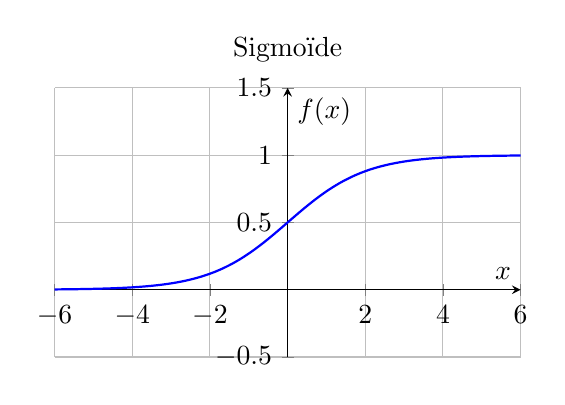
\begin{tikzpicture}
\begin{axis}[
    width=7.5cm,
    height=5cm,
    title={Sigmoïde},
    axis lines=middle,
    xlabel={$x$},
    ylabel={$f(x)$},
    xmin=-6, xmax=6,
    ymin=-0.5, ymax=1.5,
    samples=200,
    domain=-6:6,
    grid=both
]
\addplot[blue, thick] {1 / (1 + exp(-x))};
\end{axis}
\end{tikzpicture}
\end{minipage}
\hfill
\begin{minipage}{0.45\textwidth}
\centering
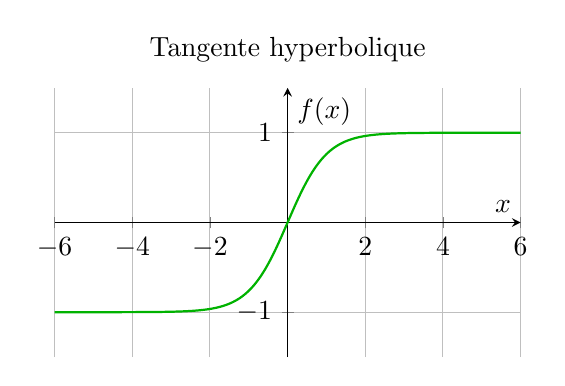
\begin{tikzpicture}
\begin{axis}[
    width=7.5cm,
    height=5cm,
    title={Tangente hyperbolique},
    axis lines=middle,
    xlabel={$x$},
    ylabel={$f(x)$},
    xmin=-6, xmax=6,
    ymin=-1.5, ymax=1.5,
    samples=200,
    domain=-6:6,
    grid=both
]
\addplot[green!70!black, thick] {tanh(x)};
\end{axis}
\end{tikzpicture}
\end{minipage}

\vspace{0.1cm}

% Deuxième ligne : ReLU & Softplus
\begin{minipage}{0.45\textwidth}
\centering
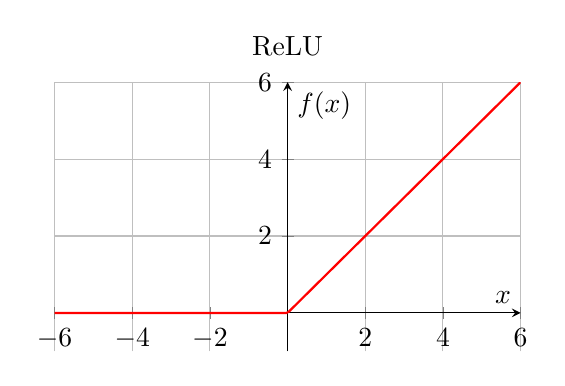
\begin{tikzpicture}
\begin{axis}[
    width=7.5cm,
    height=5cm,
    title={ReLU},
    axis lines=middle,
    xlabel={$x$},
    ylabel={$f(x)$},
    xmin=-6, xmax=6,
    ymin=-1, ymax=6,
    samples=200,
    domain=-6:6,
    grid=both
]
\addplot[red, thick] {max(0, x)};
\end{axis}
\end{tikzpicture}
\end{minipage}
\hfill
\begin{minipage}{0.45\textwidth}
\centering
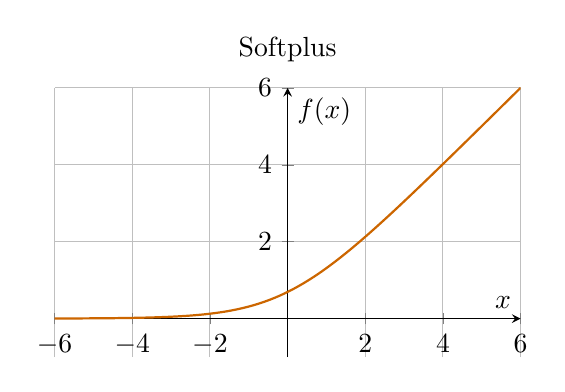
\begin{tikzpicture}
\begin{axis}[
    width=7.5cm,
    height=5cm,
    title={Softplus},
    axis lines=middle,
    xlabel={$x$},
    ylabel={$f(x)$},
    xmin=-6, xmax=6,
    ymin=-1, ymax=6,
    samples=200,
    domain=-6:6,
    grid=both
]
\addplot[orange!80!black, thick] {ln(1 + exp(x))};
\end{axis}
\end{tikzpicture}
\end{minipage}

\vspace{0.2cm}

% LIGNE 3 : Heaviside & Leaky ReLU
\begin{minipage}{0.45\textwidth}
\centering
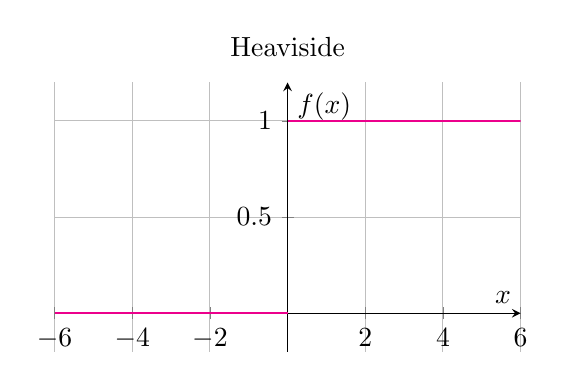
\begin{tikzpicture}
\begin{axis}[
    width=7.5cm, height=5cm,
    title={Heaviside},
    axis lines=middle,
    xlabel={$x$}, ylabel={$f(x)$},
    xmin=-6, xmax=6, ymin=-0.2, ymax=1.2,
    samples=2, domain=-6:6,
    grid=both]
\addplot[magenta, thick, domain=-6:0] {0};
\addplot[magenta, thick, domain=0.01:6] {1};
\end{axis}
\end{tikzpicture}
\end{minipage}
\hfill
\begin{minipage}{0.45\textwidth}
\centering
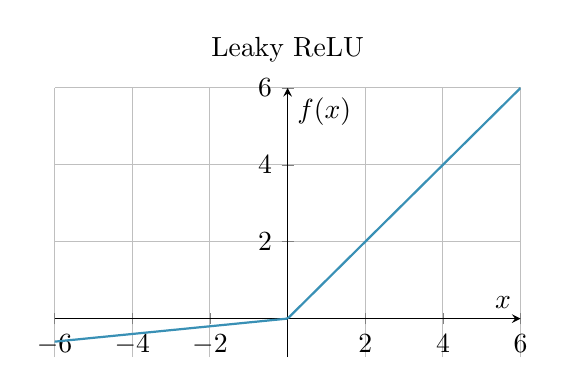
\begin{tikzpicture}
\begin{axis}[
    width=7.5cm, height=5cm,
    title={Leaky ReLU},
    axis lines=middle,
    xlabel={$x$}, ylabel={$f(x)$},
    xmin=-6, xmax=6, ymin=-1, ymax=6,
    samples=200, domain=-6:6,
    grid=both]
\addplot[cyan!70!black, thick, domain=-6:6] { (x < 0) * 0.1 * x + (x >= 0) * x };
\end{axis}
\end{tikzpicture}
\end{minipage}


    \caption{Comparaison graphique des principales fonctions d’activation}
    \label{fig:enter-label}
\end{figure}

\begin{figure}[H]
    \centering
    \begin{tikzpicture}[>=latex, thick, scale=1, every node/.style={scale=1}]

  % Entrées
  \node[draw, circle, fill=green!20!black,draw=mygreen!30!black,fill=mygreen!25] (x1) at (-2,3) {$x_1$};
  \node[draw, circle, fill=green!20!black,draw=mygreen!30!black,fill=mygreen!25] (x2) at (-2,1) {$x_2$};
  \node[draw, circle, fill=green!20!black,draw=mygreen!30!black,fill=mygreen!25] (x3) at (-2,-1) {$x_3$};

  % Sommeur
  \node[draw, circle, minimum size=1cm] (sum) at (2,1) {$\displaystyle\sum$};

  % Biais
  \node[draw, circle, minimum size=24pt] (bias) at (2.02,4.90) {};
  \node at (2.02,4.90) {$b^{(2)}_1$};
  \draw[->] (bias) -- (sum);

  % Flèches entrantes avec poids
  \draw[->] (x1) -- (sum) node[pos=0.2, yshift=11pt] {$\omega^{(2)}_{1,1}$};
  \draw[->] (x2) -- (sum) node[pos=0.2, yshift=10pt] {$\omega^{(2)}_{1,2}$};
  \draw[->] (x3) -- (sum) node[pos=0.2, yshift=13pt] {$\omega^{(2)}_{1,3}$};

  % Activation
  \node[draw, rectangle, minimum width=0.6cm, minimum height=0.6cm] (g) at (4.5,1) {$\sigma$};
  \node at (4.5,1.7) {Activation};

  \draw[->] (sum) -- (g);

  % Sorties
  \node[draw, circle, fill=red!40] (y1) at (8.5,2) {$\hat{y}_1$};
  \node[draw, circle, fill=red!40] (y2) at (8.5,0) {$\hat{y}_2$};

  \draw[->] (g) -- (y1) node[pos=0.7, yshift=12pt] {$\omega^{(3)}_{1,1}$};
  \draw[->] (g) -- (y2) node[pos=0.7, yshift=12pt] {$\omega^{(3)}_{2,1}$};

  % Cercle autour du neurone (niveau)
  % Cercle de highlight D'ABORD (au fond)
  \fill[blue!30, opacity=0.2] (3,1) circle [x radius=3cm, y radius=3cm];
  \draw[blue!60, thick] (3,1) circle [x radius=3cm, y radius=3cm];

\end{tikzpicture}

    \caption{Constitution d'un neurone pour un RNA}
    \label{fig:enter-label}
\end{figure}

La forme décrite dans l'équation \eqref{eq:perceptron} est celle d'un perceptron simple proposé par \citep{rosenblatt1957perceptron} qui est un modèle à un seul neurone, sans couche cachée. Il réalise une classification binaire en appliquant une fonction seuil à la somme pondérée des entrées où \( \theta \) est la fonction de Heaviside définie par :

\begin{equation}
\theta(z) = 
\begin{cases}
1 & \text{si } z > 0, \\
0 & \text{sinon}.
\end{cases}
\end{equation}

Ce modèle ne permet d'apprendre que des frontières de décision linéaires. Son incapacité à résoudre des problèmes non linéairement séparables, comme la fonction XOR, a motivé l’introduction des architectures plus profondes, notamment le perceptron multicouche (MLP) proposé par \citep{rumelhart1986learning} grâce à la rétroprogation du gradient.\\

Ainsi, si le neurone artificiel constitue l’unité élémentaire du calcul, c’est en les combinant au sein de couches successives que l’on construit des architectures plus expressives, capables de capturer des relations. Désormais, il faut étudier comment ces neurones sont organisés en couches et comment leur empilement donne naissance à des réseaux de neurones profonds de type feedforward.

\subsubsection{Couches cachées, architecture feedforward}

Avant de définir le MLP, il convient de mettre en exergue la notation matricielle d'un réseau de neuronnes. Soit une couche d’entrée constituée de \( n \) neurones avec activations \( \mathbf{a}^{(0)} = \left(a_1^{(0)}, a_2^{(0)}, \dots, a_n^{(0)}\right)^\top \in \mathbb{R}^n \), cette entrée est transformée par une couche cachée de \( m \) neurones selon :

\begin{equation}
\mathbf{a}^{(1)} = \sigma\left( \mathbf{\mathcal{W}}^{(0)} \mathbf{a}^{(0)} + \mathbf{b}^{(0)} \right),
\end{equation}

où :
\begin{itemize}
  \item \( \mathbf{\mathcal{W}}^{(0)} \in \mathbb{R}^{m \times n} \) est la matrice des poids de la première couche,
  \item \( \mathbf{b}^{(0)} \in \mathbb{R}^{m} \) est le vecteur des biais associés,
  \item \( \sigma(\cdot) \) est une fonction d’activation appliquée composante par composante,
  \item \( \mathbf{a}^{(1)} = \left(a_1^{(1)}, a_2^{(1)}, \dots, a_m^{(1)}\right)^\top \in \mathbb{R}^m \) est le vecteur des activations en sortie de la première couche cachée.
\end{itemize}

Chaque neurone \( a_j^{(1)} \) de la couche cachée calcule son activation via la formule :

\begin{equation}
a_j^{(1)} = \sigma\left( \sum_{i=1}^n w_{j,i}^{(0)} a_i^{(0)} + b_j^{(0)} \right),
\end{equation}

où \( w_{j,i}^{(0)} \) est le poids reliant le neurone \( i \) de la couche précédente au neurone \( j \), et \( b_j^{(0)} \) est le biais associé. Schématiquement il est obtenu la \autoref{fig:mlp_vectoriel} : 

\begin{figure}[H]
    \centering
    \begin{tikzpicture}[x=2.7cm, y=1.8cm]

  % Paramètres
  \def\NI{5} % Nombre de neurones d'entrée
  \def\NO{4} % Nombre de neurones de sortie
  \def\dyOut{1.1} % Espacement vertical de la couche de sortie
  \def\yshift{0.2} % Décalage pour les "..."

  % Couche d'entrée (espacement fixe)
  \foreach \i in {1,2,3,4}{
    \pgfmathsetmacro{\y}{\NI/2 - \i}
    \node[node in] (NI-\i) at (0,\y) {$a_{\i}^{(0)}$};
  }
  % Dernier neurone + pointillés
  \pgfmathsetmacro{\y}{\NI/2 - 5 - \yshift}
  \node[node in] (NI-5) at (0,\y) {$a_{n}^{(0)}$};
  \path (NI-5) --++ (0,1+\yshift) node[midway,scale=1.2] {$\vdots$};

  % Couche de sortie (espacement augmenté)
  \def\dy{\dyOut}
  \foreach \i in {4,3,2}{
    \pgfmathsetmacro{\y}{(\NO-1)*\dy/2 - \dy*(\i - 1)}
    \node[node] (NO-\i) at (1,\y) {$a_{\i}^{(1)}$};
    \foreach \j in {1,2,3,4,5}{
      \draw[connect,myblue!20] (NI-\j) -- (NO-\i);
    }
  }

  % Dernier neurone de sortie (en surbrillance)
  \pgfmathsetmacro{\y}{(\NO-1)*\dy/2 - \dy*(0)}
  \node[node hidden] (NO-1) at (1,\y) {$a_{m}^{(1)}$};
  \foreach \j/\label in {1/1, 2/2, 3/3, 4/4, 5/n}{
    \draw[connect,white,line width=1.2] (NI-\j) -- (NO-1);
    \draw[connect] (NI-\j) -- (NO-1)
      node[pos=0.5] {\contour{white}{$w_{1,\label}$}};
  }

  % Pointillés de sortie (placés au bon endroit)
  \path (NO-4) --++ (0,1.0) node[midway,scale=1.2] {$\vdots$};

  % Notation simplifiée
  \def\agr#1{{\color{mydarkgreen}a_{#1}^{(0)}}}

  % Équations explicites et vectorielles
  \node[below=16,right=11,mydarkblue,scale=0.95] at (NO-1)
    {$\begin{aligned}
       &= \color{mydarkred}\sigma\left( \color{black}
            w_{1,1}\agr{1} + w_{1,2}\agr{2} + \ldots + w_{1,n}\agr{n} + b_1^{(0)}
          \color{mydarkred}\right)\\
       &= \color{mydarkred}\sigma\left( \color{black}
            \sum_{i=1}^{n} w_{1,i}\agr{i} + b_1^{(0)}
           \color{mydarkred}\right)
     \end{aligned}$};

  \node[right,scale=0.9] at (1.3,-0.5)
    {$\begin{aligned}
      {\color{mydarkblue}
      \begin{pmatrix}
        a_{1}^{(1)} \\[0.3em]
        a_{2}^{(1)} \\
        \vdots \\
        a_{m}^{(1)}
      \end{pmatrix}}
      &=
      \color{mydarkred}\sigma\left[ \color{black}
      \begin{pmatrix}
        w_{1,1} & w_{1,2} & \ldots & w_{1,n} \\
        w_{2,1} & w_{2,2} & \ldots & w_{2,n} \\
        \vdots  & \vdots  & \ddots & \vdots  \\
        w_{m,1} & w_{m,2} & \ldots & w_{m,n}
      \end{pmatrix}
      {\color{mydarkgreen}
      \begin{pmatrix}
        a_{1}^{(0)} \\[0.3em]
        a_{2}^{(0)} \\
        \vdots \\
        a_{n}^{(0)}
      \end{pmatrix}}
      +
      \begin{pmatrix}
        b_{1}^{(0)} \\[0.3em]
        b_{2}^{(0)} \\
        \vdots \\
        b_{m}^{(0)}
      \end{pmatrix}
      \color{mydarkred}\right]\\[0.5em]
      {\color{mydarkblue}\mathbf{a}^{(1)}}
      &= \color{mydarkred}\sigma\left( \color{black}
           \mathbf{\mathcal{W}}^{(0)} {\color{mydarkgreen}\mathbf{a}^{(0)}}+\mathbf{b}^{(0)}
         \color{mydarkred}\right)
    \end{aligned}$};

\end{tikzpicture}

    \caption{Propagation avant dans un réseau de neurones avec une couche cachée}
    \label{fig:mlp_vectoriel}
\end{figure}

De manière générale, dans un réseau profond à \( L \) couches (hors couche d'entrée), les activations à la couche \( \ell \) (pour \( \ell = 1, \dots, L \)) sont données par la récurrence :

\begin{equation}
\mathbf{a}^{(\ell)} = \sigma^{(\ell)}\left( \mathbf{\mathcal{W}}^{(\ell-1)} \mathbf{a}^{(\ell-1)} + \mathbf{b}^{(\ell-1)} \right)
\label{eq:mlp}
\end{equation}

avec \( \mathbf{\mathcal{W}}^{(\ell-1)} \in \mathbb{R}^{m_\ell \times m_{\ell-1}} \), \( \mathbf{b}^{(\ell-1)} \in \mathbb{R}^{m_\ell} \), où \( m_\ell \) désigne le nombre de neurones à la couche \( \ell \).

La sortie finale \( \hat{\mathbf{y}} \) du réseau est alors exprimée comme :

\begin{equation}
\hat{\mathbf{y}} = \mathbf{a}^{(L)} = f(\mathbf{x}; \Theta)
\end{equation}

où \( \Theta = \{ \mathbf{\mathcal{W}}^{(\ell)}, \mathbf{b}^{(\ell)} \}_{\ell=0}^{L-1} \) désigne l’ensemble des paramètres du modèle. Un perceptron multicouche (ou \textit{Multi-Layer Perceptron}), peut alors être représenté par l'équation \eqref{eq:mlp} qui est une architecture de réseau de neurones artificiels à propagation directe (feedforward), composée d’une couche d’entrée, d’une ou plusieurs couches cachées, et d’une couche de sortie comme le montre la \autoref{fig:mlp}. Chaque couche est entièrement connectée à la suivante, sans rétroconnexion c'est ce que l'on appelle le "feed-forward". Donc, le MLP modélise une fonction \( f : \mathbb{R}^n \rightarrow \mathbb{R}^k \) par une composition de transformations affines suivies d’activations non linéaires. Pour un réseau de profondeur \( L \) avec $\mathbf{a}^{(0)} = \mathbf{x} \in \mathbb{R}^n$.  

\begin{figure}[H]
    \centering
    \begin{tikzpicture}[x=2.2cm, y=1.2cm, >=latex]

% Styles
\tikzstyle{neuron} = [circle, draw=black, thick, minimum size=25pt, inner sep=0pt]
\tikzstyle{input neuron} = [neuron, green!20!black,draw=mygreen!30!black,fill=mygreen!25]
\tikzstyle{hidden neuron 1} = [neuron, blue!20!black,draw=myblue!30!black,fill=myblue!20]
\tikzstyle{hidden neuron 2} = [neuron, blue!20!black,draw=myblue!30!black,fill=myblue!20]
\tikzstyle{output neuron} = [neuron, orange!20!black,draw=myorange!30!black,fill=myorange!20]
\tikzstyle{connect} = [draw=myblue!30]
\tikzstyle{annot} = [text width=4em, text centered]

% Nombre de neurones
\def\nI{5}
\def\nH{6}
\def\nO{2}

% Encadrement zones
\filldraw[fill=green!10, draw=green!40!black, thick, rounded corners, opacity=0.3]
  (-0.3, 0.5) rectangle (0.3, \nI + 0.5);
\node at (0, -0.6) {\sffamily \textbf{Couche d'entrée}};

\filldraw[fill=blue!10, draw=blue!60, thick, rounded corners, opacity=0.3]
  (1.2, -0.2) rectangle (3.3, \nH + 0.2);
\node at (2.2, -0.6) {\sffamily \textbf{Couches cachées}};

\filldraw[fill=orange!10, draw=orange!60, thick, rounded corners, opacity=0.3]
  (4.2, 1.5) rectangle (4.8, 5.5);
\node at (4.5, -0.6) {\sffamily \textbf{Couche de sortie}};

% Couche d'entrée
\foreach \i in {1,...,\nI}
  \node[input neuron] (I-\i) at (0, \i) {$a_{\i}^{(0)}$};

% Première couche cachée
\foreach \i in {1,...,\nH}
  \node[hidden neuron 1] (H1-\i) at (1.5, \i - 0.5) {$a_{\i}^{(1)}$};

% Deuxième couche cachée
\foreach \i in {1,...,\nH}
  \node[hidden neuron 2] (H2-\i) at (3, \i - 0.5) {$a_{\i}^{(2)}$};

% Couche de sortie (2 neurones)
\node[output neuron] (O-1) at (4.5, 5) {$\hat{y}_1$};
\node[output neuron] (O-2) at (4.5, 2) {$\hat{y}_2$};

% Connexions I -> H1
\foreach \i in {1,...,\nI}
  \foreach \j in {1,...,\nH}
    \draw[connect, thin] (I-\i) -- (H1-\j);

% Connexions H1 -> H2
\foreach \i in {1,...,\nH}
  \foreach \j in {1,...,\nH}
    \draw[connect, thin] (H1-\i) -- (H2-\j);

% Connexions H2 -> O
\foreach \i in {1,...,\nH}
  \foreach \j in {1,2}
    \draw[connect, thin] (H2-\i) -- (O-\j);

% Annotations couches
\node[align=center] at (0,6.6) {$\mathbf{x}$};
\node[align=center] at (1.5,6.6) {$\mathbf{a}^{(1)}$};
\node[align=center] at (3,6.6) {$\mathbf{a}^{(2)}$};
\node[align=center] at (4.5,6.6) {$\hat{\mathbf{y}}$};

% Étiquettes des poids
\node at (0.75,2.8) {$\mathbf{\mathcal{W}}^{(0)}$};
\node at (2.25,2.8) {$\mathbf{\mathcal{W}}^{(1)}$};
\node at (3.75,2.8) {$\mathbf{\mathcal{W}}^{(2)}$};

\end{tikzpicture}
    \caption{MLP à 2 couches cachées feedforward}
    \label{fig:mlp}
\end{figure}

Le MLP est un estimateur universel : il est capable d’approximer toute fonction mesurable à valeurs réelles avec une précision arbitraire, pourvu qu’il possède un nombre suffisant de neurones et une activation non linéaire c'est le théorème d'universalité.

\begin{theorem}[\citep{cybenko1989approximation}]
Soit \( \sigma : \mathbb{R} \rightarrow \mathbb{R} \) une fonction d’activation continue, bornée, non constante, et sigmoïde (c’est-à-dire telle que \( \lim_{x \to -\infty} \sigma(x) = 0 \) et \( \lim_{x \to +\infty} \sigma(x) = 1 \)). Alors, pour toute fonction continue \( f \in C([0,1]^n) \) et tout \( \varepsilon > 0 \), il existe un entier \( N \in \mathbb{N} \), des poids \( w_i \in \mathbb{R}^n \), des biais \( b_i \in \mathbb{R} \) et des coefficients \( \alpha_i \in \mathbb{R} \) tels que la fonction :

\begin{equation}
\hat{f}(x) = \sum_{i=1}^{N} \alpha_i \, \sigma(w_i^\top x + b_i)
\end{equation}

vérifie :
\begin{equation}
\sup_{x \in [0,1]^n} \left| f(x) - \hat{f}(x) \right| < \varepsilon.
\end{equation}
\end{theorem}

Autrement dit, un réseau de neurones à une seule couche cachée contenant un nombre suffisant de neurones, utilisant une fonction d’activation sigmoïde, peut approximer toute fonction continue sur un compact de \( \mathbb{R}^n \), à une précision arbitraire. Ce théorème a été étendu à d'autres fonctions d’activation (comme ReLU, tanh) et à d’autres classes de fonctions cibles (espaces \( L^p \), fonctions mesurables, etc.). Il fournit une justification théorique majeure à l'utilisation des MLP pour l'apprentissage supervisé.\\

Une fois présenté la structure interne des réseaux de neurones, depuis l’unité de base (le neurone artificiel) jusqu’aux architectures profondes de type perceptron multicouche. Cette modélisation reste cependant statique tant que les paramètres ne sont pas ajustés. La section suivante introduit donc le processus d’apprentissage, au cœur du fonctionnement de ces modèles, en détaillant les algorithmes d’optimisation qui permettent d’ajuster les poids pour minimiser l’erreur de prédiction.

\subsection{Apprentissage et optimisation}

L’apprentissage des réseaux de neurones repose sur l’ajustement progressif de leurs paramètres internes (principalement les poids et les biais) afin de minimiser une fonction de coût mesurant l’écart entre les prédictions du modèle et les valeurs cibles issues des données d’entraînement. Ce processus repose sur des méthodes d’optimisation numérique, souvent itératives, permettant d’orienter le modèle vers une solution qui généralise correctement aux données non vues. Les principes fondamentaux de l’optimisation dans les réseaux de neurones seront exposés. L’accent sera d’abord mis sur l’algorithme de descente de gradient, qui constitue le cadre de base de la plupart des méthodes d’apprentissage. Ses variantes, telles que la descente stochastique, le mini-batch, ou encore les algorithmes à mémoire comme le momentum et Adam\footnote{En deep learning, Adam est un algorithme d’optimisation très populaire, utilisé pour entraîner les réseaux de neurones. Son nom signifie Adaptive Moment Estimation.}, seront introduites afin de mieux répondre aux architectures profondes. Ensuite, l’algorithme de rétropropagation du gradient, essentiel pour l’entraînement efficace des réseaux multicouches, sera ensuite formellement détaillé. Ce mécanisme permet de propager les erreurs depuis la couche de sortie vers les couches précédentes, afin de calculer les dérivées partielles requises pour la mise à jour des paramètres. Enfin, les principales techniques de régularisation utilisées pour lutter contre le surapprentissage seront présentées. Il sera notamment question de la régularisation $\ell^2$, du dropout, de la batch normalization et de l’early stopping. Ces méthodes visent à améliorer la capacité du réseau à généraliser, tout en assurant une meilleure stabilité de l’apprentissage.

\subsubsection{Descente de gradient et variantes}

L'algorithme de descente de gradient est une méthode itérative d'optimisation permettant de minimiser une fonction différentiable \( E: \mathbb{R}^d \to \mathbb{R} \). Dans le cadre de l'apprentissage supervisé par réseaux de neurones, \( E \) représente généralement une fonction de coût (ou fonction de perte) mesurant l'écart entre les sorties prédites par le modèle et les valeurs cibles issues des données d’entraînement.

Soit un vecteur de paramètres (ou poids) \( \boldsymbol{w} \in \mathbb{R}^d \), l'objectif est de résoudre :
\begin{equation}
    \min_{\boldsymbol{w} \in \mathbb{R}^d} E(\boldsymbol{w})
\end{equation}

La descente de gradient consiste à effectuer, à chaque itération \( t \in \mathbb{N} \), une mise à jour du vecteur \( \boldsymbol{w} \) selon :
\begin{equation}
    \boldsymbol{w}^{(t+1)} = \boldsymbol{w}^{(t)} - \lambda_t \nabla E(\boldsymbol{w}^{(t)}),
\end{equation}

où \( \lambda_t > 0 \) est le \textit{taux d’apprentissage} (ou pas de descente), et \( \nabla E(\boldsymbol{w}^{(t)}) \) est le gradient de \( E \) évalué en \( \boldsymbol{w}^{(t)} \).

Lorsque la fonction \( E \) est \( \mathcal{C}^1 \) (continûment différentiable), le gradient \( \nabla E(\boldsymbol{w}) \) pointe vers la direction de plus forte croissance locale de \( E \), et son opposé vers la direction de la décroissance maximale. 

Sous certaines conditions sur \( E \) (forte convexité, Lipschitzianité du gradient), la suite \( (\boldsymbol{w}^{(t)})_{t \in \mathbb{N}} \) converge vers un minimum local, voire global si \( E \) est convexe.

\paragraph{Convergence (cas convexe)} Si \( E \) est \( L \)-Lipschitz-gradient et \( \lambda_t = \lambda \in (0, 1/L) \), alors la descente de gradient vérifie :
\begin{equation}
    E(\boldsymbol{w}^{(t)}) - E(\boldsymbol{w}^*) \leq \frac{\| \boldsymbol{w}^{(0)} - \boldsymbol{w}^* \|^2}{2\lambda t}
\end{equation}

où \( \boldsymbol{w}^* \) est un minimum global.

\paragraph{Application aux réseaux de neurones} 
Dans le cas d’un réseau de neurones, il est noté \( w_{ij}^{(\ell)} \) le poids connectant le neurone \( j \) de la couche \( \ell-1 \) au neurone \( i \) de la couche \( \ell \). La mise à jour associée à ce paramètre est alors donnée par :
\begin{equation}
    w_{ij}^{(\ell)} \leftarrow w_{ij}^{(\ell)} - \lambda \cdot \frac{\partial E}{\partial w_{ij}^{(\ell)}}
\end{equation}

avec :
\begin{equation}
    \frac{\partial E}{\partial w_{ij}^{(\ell)}} = e_i^{(\ell)} \cdot a_j^{(\ell-1)},
\end{equation}

où \( e_i^{(\ell)} \) est l’erreur rétropropagée (\autoref{sec:retropropagation}) au neurone \( i \) de la couche \( \ell \), et \( a_j^{(\ell-1)} \) l’activation du neurone \( j \) de la couche précédente. Cette formulation résulte directement de l'application de la règle de la chaîne. Ce schéma est à la base de l'entraînement de tout réseau de neurones via rétropropagation, et constitue le socle de nombreuses variantes comme la descente de gradient stochastique (SGD), le momentum ou Adam, présentées ci-dessous.

\paragraph{Descente de gradient stochastique (SGD)}
Au lieu de calculer le gradient complet \( \nabla E \) sur l’ensemble du jeu de données, il est effectué la mise à jour après chaque exemple \( (x^{(i)}, t^{(i)}) \) :
\begin{equation}
    \boldsymbol{w}^{(t+1)} = \boldsymbol{w}^{(t)} - \lambda \nabla E^{(i)}(\boldsymbol{w}^{(t)})
\end{equation}
Cela introduit du bruit bénéfique pour sortir de certains minima locaux et permet des itérations plus rapides.

\paragraph{Mini-batch gradient descent}
Il est utilisé une moyenne des gradients sur un sous-ensemble \( \mathcal{B} \) d’exemples (batch de taille \( B \)) :
\begin{equation}
    \boldsymbol{w}^{(t+1)} = \boldsymbol{w}^{(t)} - \lambda \cdot \frac{1}{B} \sum_{i \in \mathcal{B}} \nabla E^{(i)}(\boldsymbol{w}^{(t)})
\end{equation}
Cela stabilise l’apprentissage tout en conservant une efficacité computationnelle.

\paragraph{Momentum}
Ici, il ya l'introduction d'une "vitesse" \( \boldsymbol{v}^{(t)} \) accumulant les gradients :
\begin{align}
    \boldsymbol{v}^{(t+1)} &= \beta \boldsymbol{v}^{(t)} - \lambda \nabla E(\boldsymbol{w}^{(t)}) \\
    \boldsymbol{w}^{(t+1)} &= \boldsymbol{w}^{(t)} + \boldsymbol{v}^{(t+1)}
\end{align}
\( \beta \in [0,1] \) contrôle l’inertie. Cela permet d’accélérer la convergence et d’atténuer les oscillations dans des vallées de la fonction de coût.

\paragraph{Adam (Adaptive Moment Estimation)}
Algorithme qui combine l’adaptativité d’AdaGrad avec l’effet mémoire du momentum. Il maintient deux estimations :
\begin{align}
    m_t &= \beta_1 m_{t-1} + (1 - \beta_1) \nabla E(\boldsymbol{w}^{(t)}) \\
    v_t &= \beta_2 v_{t-1} + (1 - \beta_2) \left[\nabla E(\boldsymbol{w}^{(t)})\right]^2
\end{align}
Après correction du biais :
\begin{equation}
    \boldsymbol{w}^{(t+1)} = \boldsymbol{w}^{(t)} - \lambda \cdot \frac{\hat{m}_t}{\sqrt{\hat{v}_t} + \varepsilon},
\end{equation}
avec :
\begin{equation}
    \hat{m}_t = \frac{m_t}{1 - \beta_1^t}, \quad \hat{v}_t = \frac{v_t}{1 - \beta_2^t}
\end{equation}
Adam est aujourd’hui l’algorithme d’optimisation par défaut dans de nombreux contextes de deep learning.\\

Les méthodes d’optimisation présentées précédemment reposent toutes sur la capacité à calculer efficacement les dérivées partielles de la fonction de coût par rapport aux paramètres du réseau. Cette opération est rendue possible grâce à l’algorithme de rétropropagation du gradient, qui permet de propager l’erreur de la sortie vers les couches cachées du réseau tout en respectant la structure différentiable du modèle. 

\subsubsection{Algorithme de rétropropagation du gradient}\label{sec:retropropagation}

L'algorithme de rétropropagation du gradient (ou 	\textit{backpropagation}) \citep{lecun1998gradient} permet de minimiser l'erreur entre la sortie réelle du réseau et la sortie attendue sur un ensemble de données d’apprentissage. Le principe est d’ajuster les poids synaptiques du réseau de neurones à l’aide d’un algorithme de descente de gradient, en calculant les dérivées partielles de la fonction de perte par rapport à chaque poids.

\newpage

Soit \( \textbf{a}^{(0)}=\mathbf{x} \in \mathbb{R}^n \) un vecteur d'entrée et \( \mathbf{\widehat{y}} \in \mathbb{R}^m \) le vecteur cible (sortie désirée). Chaque couche \( \ell \in \{1, \dots, L\} \) du réseau transforme les activations de la couche précédente \( \mathbf{a}^{(\ell-1)} \) en activations \( \mathbf{a}^{(\ell)} \) selon :

\begin{equation}
\mathbf{z}^{(\ell)} = \mathbf{\mathcal{W}}^{(\ell)} \mathbf{a}^{(\ell-1)} + \mathbf{b}^{(\ell)}, \quad  \mathbf{a}^{\ell}=\sigma^{(\ell)}\left(\mathbf{z}^{(\ell)}\right)
\end{equation}

où \( \sigma^{(\ell)} \) est la fonction d’activation de la couche \( \ell \). Soit en écriture non matricielle : 

\begin{equation}
     z_{j}^{(\ell)}=\sigma^{(\ell)}{\Big (}\sum _{k}w_{jk}^{(\ell)}a_{k}^{(\ell-1)}{\Big )},
\quad  a_{j}^{(\ell)}=\sigma^{(\ell)}\left(z_{j}^{(\ell)} \right )
\end{equation}

En utilisant ensuite les erreurs propagées pour calculer le gradient de la fonction de coût \( \mathcal{L} \), définie par :

\begin{equation}
\mathcal{L} = \frac{1}{2} \sum_{i=1}^{m} \left( y_i - \widehat{y}_i \right)^2
\end{equation}

À la couche de sortie, il est défini le vecteur de sortie \( \mathbf{y} = \mathbf{a}^{(L)} \), et l'erreur est donnée par :

\begin{equation}
\frac{\partial \mathcal{L}}{\partial z_i^{\text{sortie}}} = \frac{\partial \displaystyle{\left (\frac{1}{2}  \sum_{k} \left ( y_i-\sigma(z_i^{\text{sortie}}) \right )^2 \right )}}{\partial z_i^{\text{sortie}}}
=e_i^{\text{sortie}} = \sigma'(z_i^{\text{sortie}})(y_i-\widehat{y_i})
\end{equation}

Pour chaque couche \( \ell = L-1, L-2, \dots, 1 \), l'erreur se propage vers l’arrière selon :

\begin{equation}
{\displaystyle e_{j}^{(\ell-1)}=g'^{(\ell-1)}(z_{j}^{(\ell-1)})\sum _{i}w_{ij}^{(\ell)}e_{i}^{(\ell)}}
\end{equation}

Le gradient de \( \mathcal{L} \) par rapport aux poids \( w_{ij}^{(\ell)} \) est donné par :

\begin{equation}
\frac{\partial \mathcal{L}}{\partial w_{ij}^{(\ell)}} 
=
\frac{\partial \mathcal{L}}{\partial a^{(\ell)}_i} \times \frac{\partial a^{(\ell)}_i}{\partial z_i^{(\ell)}} \times \frac{\partial z_i^{(\ell)}}{\partial w_{ij}^{(\ell)}}
= e_i^{(\ell)} a_j^{(\ell-1)}
\end{equation}

Chaque poids est alors mis à jour selon la règle :

\begin{equation}
w_{ij}^{(\ell)} \leftarrow w_{ij}^{(\ell)} - \lambda \frac{\partial \mathcal{L}}{\partial w_{ij}^{(\ell)}} = w_{ij}^{(\ell)} - \lambda e_i^{(\ell)} a_j^{(\ell-1)}
\end{equation}

où \( \lambda \in (0,1) \) est le taux d'apprentissage.

\newpage

\begin{demonstration}
Soit $L \in \mathbb{N}^*$ le nombre de couches (à l'exclusion de la couche d'entrée).  
Soient $d_0, d_1, \dots, d_L \in \mathbb{N}^*$ les dimensions de chaque couche.

\medskip

Paramètres : Pour chaque $\ell \in \{1, \dots, L\}$ :
\begin{itemize}
    \item $\mathcal{W}^{(\ell)} \in \mathbb{R}^{d_\ell \times d_{\ell-1}}$ : matrice de poids
    \item $b^{(\ell)} \in \mathbb{R}^{d_\ell}$ : vecteur de biais
    \item $\phi^{(\ell)} : \mathbb{R}^{d_\ell} \to \mathbb{R}^{d_\ell}$ : fonction d’activation non-linéaire
\end{itemize}
\medskip

Propagation avant :
\[
\begin{aligned}
a^{(0)} &= x \in \mathbb{R}^{d_0} \\
z^{(\ell)} &= \mathcal{W}^{(\ell)} a^{(\ell-1)} + b^{(\ell)} \\
a^{(\ell)} &= \phi^{(\ell)}(z^{(\ell)}) \quad \text{pour } \ell = 1, \dots, L
\end{aligned}
\]

Fonction du réseau de neurones :
\[
f_\theta(x) := a^{(L)}, \quad \theta = \{ (\mathcal{W}^{(\ell)}, b^{(\ell)}) \}_{\ell=1}^{L}
\]

Définissons le terme d’erreur pour chaque couche $\ell$ du réseau :
\[
\delta^{(\ell)} := \frac{\partial \mathcal{L}}{\partial z^{(\ell)}} \in \mathbb{R}^{d_\ell}
\]

\medskip

Pour la dernière couche, lorsque la fonction de perte est : $\mathcal{L}(a^{[L]}, y)$, on applique la règle de dérivation en chaîne :
\[
\delta^{(L)} = \frac{\partial \mathcal{L}}{ \partial z^{(L)}} = \frac{\partial \mathcal{L}}{ \partial a^{(L)}} \times \frac{\partial a^{(L)}}{ \partial z^{(L)}}
\]
ce qui donne :
\[
\delta^{(L)} = \nabla_{a^{(L)}} \mathcal{L} \circ \phi^{(L)'}(z^{(L)})
\]

où $\nabla_{a^{(L)}} \mathcal{L} = a^{(L)} - y$ (cas d'une perte quadratique).

\medskip

Étape récursive pour $\ell = L-1, \dots, 1$ : on commence par cette dérivée :
\[
\frac{\partial \mathcal{L}}{\partial a^{(\ell)}} 
= \left( \frac{\partial \mathcal{L}}{\partial z^{(\ell+1)}} \cdot \frac{\partial z^{(\ell+1)}}{\partial a^{(\ell)}} \right) 
= \delta^{(\ell+1)} \cdot \mathcal{W}^{(\ell+1)}
\]
Le terme d’erreur devient alors :
\[
\delta^{(\ell)} = \left( \mathcal{W}^{(\ell+1)^\top} \delta^{(\ell+1)} \right) \circ \phi^{(\ell)'}(z^{(\ell)})
\]

\medskip

Gradients des paramètres :
\[
\begin{aligned}
\frac{\partial \mathcal{L}}{\partial \mathcal{W}^{(\ell)}} &= \delta^{(\ell)} (a^{(\ell-1)})^\top, \quad \frac{\partial \mathcal{L}}{\partial b^{(\ell)}} = \delta^{(\ell)}
\end{aligned}
\]
\end{demonstration}

Ce résultat permet de calculer efficacement tous les gradients par propagation en arrière, sans recalculer l’ensemble des dérivées individuellement. Bien que l’algorithme de rétropropagation permette d’entraîner efficacement les réseaux de neurones en ajustant les paramètres selon le gradient de l’erreur, il ne garantit pas à lui seul une bonne généralisation. En pratique, les réseaux profonds possèdent une très grande capacité d’approximation, ce qui les rend particulièrement sensibles au surapprentissage. Il est donc nécessaire d’introduire des mécanismes de régularisation afin de prévenir ce phénomène et d’assurer une performance stable sur des données nouvelles.

\subsubsection{Régularisation et techniques d'évitement du surapprentissage}

L’un des défis majeurs en apprentissage profond est d’éviter le \textit{surapprentissage} (\textit{overfitting}), c’est-à-dire une trop forte mémorisation des données d’entraînement, au détriment de la généralisation. Plusieurs techniques de régularisation sont employées pour contrôler la capacité du modèle :

\begin{itemize}
    \item \textbf{Régularisation \( \ell^2 \) (ridge)} : cela consiste à ajouter un terme \( \lambda \|\mathbf{\mathcal{W}}\|_2^2 \) à la fonction de coût pour pénaliser les poids trop grands. La fonction de coût devient :
    \begin{equation}
        \mathcal{L}_{reg} = \mathcal{L} + \frac{\lambda}{2} \sum_{l} \sum_{i,j} \left(w_{ij}^{(l)}\right)^2
    \end{equation}
    \item \textbf{Régularisation \( \ell^1 \) (lasso)} : favorise la parcimonie en ajoutant \( \displaystyle{\lambda \sum |w_{ij}^{(l)}}| \) à la fonction de coût.
    \item \textbf{Dropout} : technique stochastique où, à chaque itération, certains neurones (et leurs connexions) sont ignorés avec une probabilité \( p \). Cela évite que le réseau ne devienne dépendant de chemins particuliers.
    \item \textbf{Early stopping} : surveillance de la performance sur un ensemble de validation. Si l'erreur de validation augmente pendant que celle d’entraînement baisse, l’apprentissage s'arrête.
    \item \textbf{Batch Normalization} : normalise les activations intermédiaires pour accélérer l'apprentissage et réduire la sensibilité à l'initialisation.
\end{itemize}

Combinées aux techniques d’optimisation précédentes, ces méthodes permettent d’améliorer significativement la robustesse et la performance des réseaux de neurones.\\

En somme, les réseaux de neurones artificiels constituent un cadre mathématique général pour l'apprentissage supervisé, fondé sur la composition de couches linéaires et non linéaires. La structure des MLP, combinée à des fonctions d’activation adéquates et à des algorithmes d’optimisation efficaces tels que la rétropropagation du gradient, permet d’approximer une grande variété de fonctions cibles avec une précision arbitraire. L’introduction de techniques de régularisation comme le dropout, la normalisation de batch ou l’arrêt anticipé a permis d’améliorer significativement la robustesse et la capacité de généralisation de ces modèles, ouvrant la voie à des architectures plus profondes.\\

Cependant, malgré leur expressivité, les MLP traditionnels peinent à capturer efficacement les dépendances structurelles à long terme présentes dans certaines données séquentielles ou textuelles. C’est dans ce contexte que les architectures à attention, et en particulier les Transformers, ont été introduites. Proposés initialement pour les tâches de traitement du langage naturel par \citep{vaswani2017attention}, les Transformers ont rapidement révolutionné le domaine de l’apprentissage profond, en exploitant un mécanisme d’attention permettant de traiter simultanément l’ensemble des entrées sans recours à la récurrence. Le paragraphe suivant est donc consacré à l’étude détaillée de cette architecture, de ses fondements théoriques à ses applications contemporaines.

\section{Transformers}

Depuis leur introduction par \citep{vaswani2017attention}, les Transformers ont profondément bouleversé l’intelligence artificielle, en particulier dans le traitement automatique du langage naturel (TALN ou NLP). L’article fondateur Attention is All You Need a inauguré une architecture novatrice fondée exclusivement sur des mécanismes d’attention, rompant avec les approches séquentielles traditionnelles basées sur les réseaux récurrents ou convolutionnels. En modélisant les dépendances contextuelles à travers une attention globale, parallélisable et différentiable, les Transformers ont permis des gains considérables en efficacité computationnelle, en performance de généralisation, et en scalabilité sur de grandes quantités de données. Cette architecture a rapidement donné naissance à une série de modèles pré-entraînés de plus en plus puissants, tels que BERT \citep{devlin2018bert}, GPT \citep{radford2018gpt1,radford2019gpt2}, RoBERTa \citep{liu2019roberta}, T5 \citep{raffel2020t5}, ou encore DeBERTa \citep{he2021deberta}, établissant les Transformers comme le modèle des systèmes d’IA contemporains.\\

Le succès des Transformers repose sur plusieurs aspects : la représentation distribuée des mots sous forme de vecteurs continus (embeddings), l’attention multi-tête permettant l’agrégation d’information contextuelle hétérogène, et une structure encodeur/décodeur adaptée à une large variété de tâches. Ce paragraphe traite donc  en profondeur ces composantes architecturales, en mettant en évidence les innovations mathématiques et algorithmiques sous-jacentes. Après avoir décrit les mécanismes de tokenisation et d'encodage positionnel, l'attention sera portée sur les principes du self-attention, puis sur l'extension multi-head. Enfin, les encodeurs bidirectionnels tels que BERT et les variantes modernes comme ModernBERT \citep{warner2024modernbert} seront analysés, afin de comprendre les évolutions récentes des modèles de représentation contextuelle dans le cadre de l'apprentissage profond.

\subsection{L'architecture}

L’efficacité des Transformers repose sur une architecture articulée autour de trois mécanismes fondamentaux : la représentation vectorielle des entrées, l’attention multi-tête, et la structuration modulaire en blocs encodeurs et décodeurs. Contrairement aux réseaux neuronaux traditionnels, qui traitent les données séquentiellement, les Transformers adoptent un traitement global et parallèle des séquences, ce qui favorise une meilleure captation des dépendances à longue portée. Les différentes composantes architecturales des Transformers seront introduites progressivement. Il sera d’abord question des représentations vectorielles, de la tokenisation et des embeddings positionnels, éléments fondamentaux pour projeter le texte brut dans un espace numérique exploitable. Ensuite, les mécanismes d’attention (en particulier le \textit{self-attention} et son extension \textit{multi-head}) seront étudiés en détail, avant de conclure sur la structure globale encodeur-décodeur.

\subsubsection{Représentations vectorielles, tokenisation et embeddings} 

Dans l’architecture Transformer, comme dans la plupart des modèles de traitement du langage naturel modernes, les mots ne sont pas directement traités sous leur forme brute (c'est-à-dire sous forme textuelle), mais sous forme de représentations vectorielles continues appelées embeddings. Avant d’être transformés en embeddings, les textes bruts sont d’abord découpés en unités appelées \textit{tokens}, via un processus de tokenisation (Figure \ref{fig:tokenization_example}). Contrairement à la simple séparation en mots, les modèles modernes utilisent des méthodes de tokenisation sous-morphologique, telles que Byte-Pair Encoding (BPE) ou WordPiece, qui permettent de représenter efficacement des mots rares ou inconnus à l’aide de sous-unités fréquentes. 

\begin{figure}[H]
    \centering
    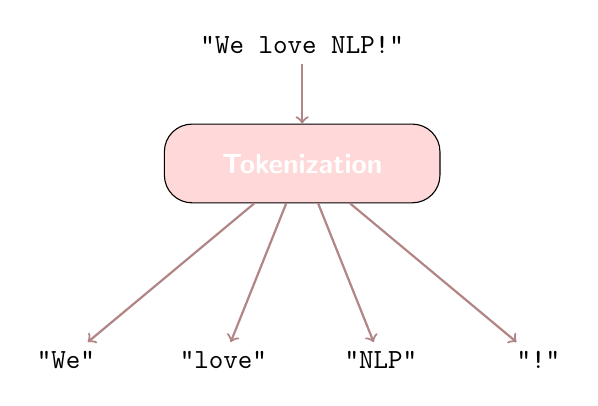
\begin{tikzpicture}[every node/.style={font=\sffamily}, node distance=1.2cm and 2cm, align=center]
        % Sentence input
        \node (sentence) at (0, 4) {\texttt{"We love NLP!"}};

        % Tokenization box
        \node[draw, rounded corners=10pt, fill=pink!60, text=white, minimum width=3.5cm, minimum height=1cm] (tokenization) at (0, 2.5) {\textbf{Tokenization}};

        % Tokens on a straight line
        \node (we) at (-3, 0) {\texttt{"We"}};
        \node (love) at (-1, 0) {\texttt{"love"}};
        \node (nlp) at (1, 0) {\texttt{"NLP"}};
        \node (punct) at (3, 0) {\texttt{"!"}};

        % Arrows
        \draw[->, thick, pink!70!black] (sentence) -- (tokenization);
        \draw[->, thick, pink!70!black] (tokenization) -- (we);
        \draw[->, thick, pink!70!black] (tokenization) -- (love);
        \draw[->, thick, pink!70!black] (tokenization) -- (nlp);
        \draw[->, thick, pink!70!black] (tokenization) -- (punct);
\end{tikzpicture}
    \caption{Illustration du processus de tokenisation simple : transformation d'une phrase en unités élémentaires (tokens)}
    \label{fig:tokenization_example}
\end{figure}

Chaque token est ensuite associé à un vecteur dense appris, formant ainsi la base des embeddings d'entrée du modèle. Ces embeddings capturent des propriétés sémantiques et syntaxiques des mots, en projetant les termes dans un espace vectoriel (Figure \ref{fig:embedding_example}) où les distances entre vecteurs reflètent la proximité sémantique.

\begin{figure}[H]    
    \centering
    \begin{tikzpicture}[scale=0.8, every node/.style={scale=0.8}]
        % Input Objects
        \node[draw, rectangle, rounded corners, fill=blue!10] (obj1) at (0, 2) {Token 1};
        \node[draw, rectangle, rounded corners, fill=blue!10] (obj2) at (0, 0) {Token 2};
        \node[draw, rectangle, rounded corners, fill=blue!10] (obj3) at (0, -2) {Token 3};

        % Embedding Model
        \node[draw, diamond, aspect=2, fill=purple!10, minimum width=4cm, minimum height=4cm] (embed) at (4, 0) {Embedding Model};

        % Embedding Vectors
        \node[draw, rectangle, rounded corners, fill=purple!5] (vec1) at (9, 2) {[0.12, 0.75, -0.33 ...]};
        \node[draw, rectangle, rounded corners, fill=purple!5] (vec2) at (9, 0) {[0.85, 0.21, 0.88 ...]};
        \node[draw, rectangle, rounded corners, fill=purple!5] (vec3) at (9, -2) {[-0.05, 0.68, 0.5 ...]};

        % Vector labels
        \node[fill=gray!20] at (12, 2) {Vector 1};
        \node[fill=gray!20] at (12, 0) {Vector 2};
        \node[fill=gray!20] at (12, -2) {Vector 3};

        % Arrows
        \draw[->, thick] (obj1) -- (embed);
        \draw[->, thick] (obj2) -- (embed);
        \draw[->, thick] (obj3) -- (embed);

        \draw[->, thick] (embed) -- (vec1);
        \draw[->, thick] (embed) -- (vec2);
        \draw[->, thick] (embed) -- (vec3);
\end{tikzpicture}
    \caption{Schéma d'un modèle d'embedding transformant des objets en vecteurs numériques}
    \label{fig:embedding_example}
\end{figure}

Historiquement, les embeddings les plus connus tels que Word2Vec \citep{mikolov2013distributed,mikolov2013efficient} et GloVe \citep{pennington2014glove} ont permis des avancées majeures dans le NLP en démontrant que les relations entre mots peuvent être capturées dans un espace vectoriel continu. FastText \citep{bojanowski2017enriching,joulin2017bag} a ensuite étendu ces approches en incorporant des informations sous-morphologiques, améliorant ainsi les représentations pour les langues morphologiquement riches ou pour des mots rares.\\

Dans le cadre des Transformers, une innovation supplémentaire a été introduite avec les positional embeddings \citep{vaswani2017attention}, essentiels pour compenser l'absence de structure récurrente qui fournissait initialement l'information sur l'ordre des mots dans des modèles comme les RNN \citep{hochreiter1997long,cho2014learning}. Les positional embeddings permettent aux Transformers d’intégrer l'information de séquence, en ajoutant aux embeddings classiques des informations de position des mots dans la séquence d'entrée. Chaque position $p$ est encodée par une paire de valeurs $[\sin(\omega_i p), \cos(\omega_i p)]$ pour chaque dimension $i$, où $\omega_i = 1 / 10000^{2i/d}$ \citep{vaswani2017attention} définit une progression géométrique des fréquences. Il faut obtenir une matrice $\mathcal{M}_k$ qui applique un décalage de $k$ positions à une position $p$, c'est-à-dire :

\begin{equation}
\mathcal{M}_k \cdot \begin{bmatrix} \sin(\omega_i p) \\ \cos(\omega_i p) \end{bmatrix} = \begin{bmatrix} \sin(\omega_i (p + k)) \\ \cos(\omega_i (p + k)) \end{bmatrix}
\end{equation}

En appliquant les formules de somme d'angles :
\begin{align*}
\sin(\omega_i(p + k)) &= \sin(\omega_i p)\cos(\omega_i k) + \cos(\omega_i p)\sin(\omega_i k) \\
\cos(\omega_i(p + k)) &= \cos(\omega_i p)\cos(\omega_i k) - \sin(\omega_i p)\sin(\omega_i k)
\end{align*}

Il est posible d'écrire le décalage comme une multiplication matricielle :

\begin{equation}
\mathcal{M}_k = \begin{bmatrix} \cos(\omega_i k) & \sin(\omega_i k) \\ -\sin(\omega_i k) & \cos(\omega_i k) \end{bmatrix}
\end{equation}

Cette matrice $M_k$ est une matrice de rotation classique en dimension 2. Cela signifie que le déplacement d'un token de $k$ positions correspond à une rotation de son embedding positionnel sur le cercle unité. Les positional embeddings sinusoïdaux permettent une modélisation naturelle des relations relatives entre tokens, pas seulement des positions absolues. C'est cette propriété qui inspire les encodages positionnels plus récents comme RoPE (Rotary Positional Embedding), où les relations sont explicitement décodées comme des rotations.\\

Les modèles ultérieurs basés sur Transformers, comme BERT \citep{devlin2018bert}, utilisent également des embeddings spécifiques pour différencier les segments dans les tâches impliquant plusieurs phrases, ainsi que des embeddings spéciaux pour dénoter le début ou la fin des séquences, augmentant davantage la richesse expressive de leurs représentations. Une fois les entrées textuelles converties en représentations vectorielles enrichies, il devient nécessaire de modéliser leurs interactions contextuelles. C’est précisément le rôle du mécanisme de self-attention, l'apport des Transformers, qui permet à chaque élément de la séquence d’adapter dynamiquement sa représentation en fonction de l’ensemble des autres tokens.

\subsubsection{Self-attention}

Le mécanisme de \textit{self-attention} est l'apport principal de l'architecture Transformer \citep{vaswani2017attention}. Il permet à chaque token d'une séquence d'interagir avec tous les autres, en pondérant leur influence respective pour produire une nouvelle représentation enrichie du contexte global.\\

L'idée est de calculer, pour chaque token, une représentation pondérée de tous les autres tokens de la séquence. Cette pondération est déterminée de manière dynamique, selon leur pertinence contextuelle. Autrement dit, un mot va « regarder » les autres mots et « décider » de l’importance de chacun dans son propre encodage.\\

Chaque vecteur d'entrée $x_i$ est projeté linéairement dans trois espaces vectoriels : les requêtes $Q$, les clés $K$ et les valeurs $V$ :
\begin{equation}
Q = \mathbf{X}\mathcal{W}^Q, \quad K = \mathbf{X}\mathcal{W}^K, \quad V = \mathbf{X}\mathcal{W}^V
\end{equation}
où $\mathbf{X} \in \mathbb{R}^{n \times d_{model}}$ est la matrice des embeddings d'entrée, et $\mathcal{W}^Q$, $\mathcal{W}^K$, $\mathcal{W}^V$ sont des matrices de poids. Ensuite les scores d'attention sont calculés par le produit scalaire entre chaque requête et toutes les clés :

\begin{equation}
\text{score}_{ij} = \frac{Q_i \times K_j^T}{\sqrt{d_k}}
\end{equation}

puis il est appliqué une softmax pour normaliser les scores :

\begin{equation}
\alpha_{ij} = \text{softmax}(\text{score}_{ij})
\end{equation}

La sortie est une combinaison pondérée des vecteurs de valeurs :
\begin{equation}
\text{Attention}(Q, K, V) = \text{softmax}\left(\frac{QK^T}{\sqrt{d_k}}\right)V 
\end{equation}

Le mécanisme d'attention capture les dépendances longues distances de manière efficace, il est parallélisable contrairement aux RNN, ce qui accélère considérablement l'entraînement. Enfin, il permet une meilleure interprétabilité grâce aux poids d’attention. La procédure peut ainsi être vue schématiquement dans la Figure \ref{fig:self_attention_diagram}.

\begin{figure}[H]
    \centering
        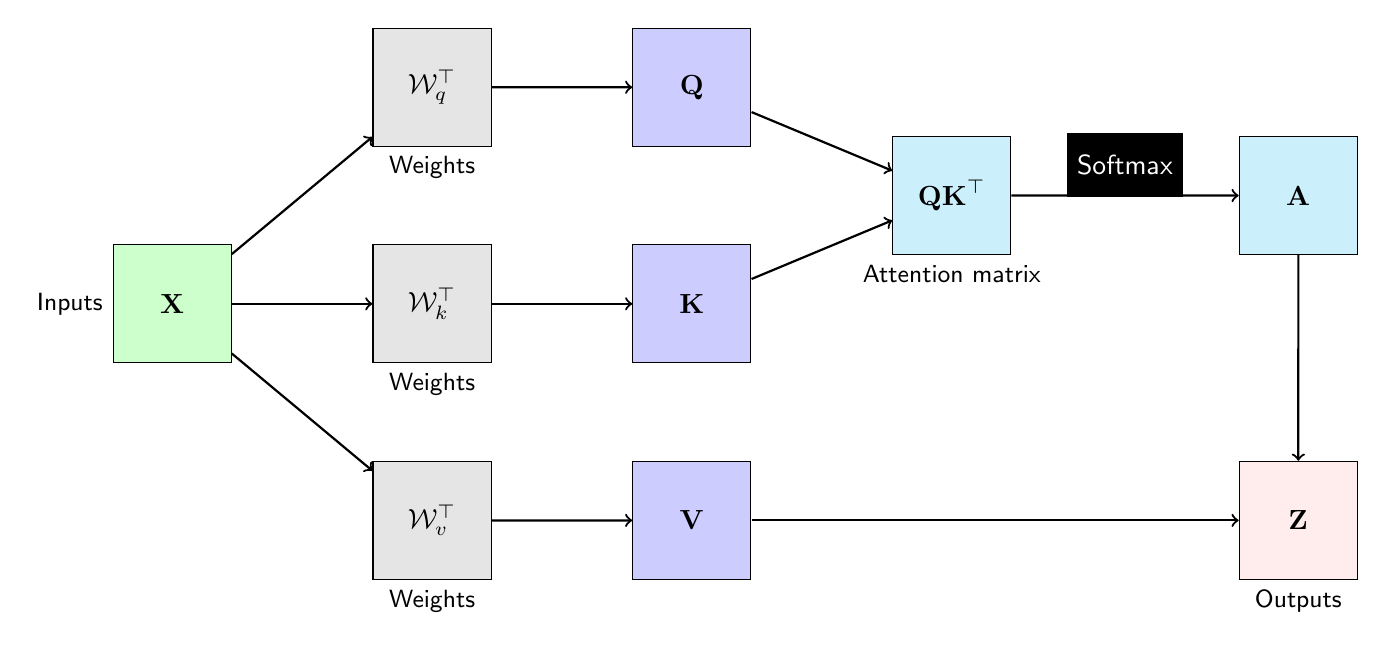
\begin{tikzpicture}[every node/.style={font=\sffamily, align=center}, box/.style={draw, minimum height=1.5cm, minimum width=1.5cm}, scale=1.1]
        % Input X
        \node[box, fill=green!20, label=left:{\small Inputs}] (x) at (0,0) {$\mathbf{X}$};

        % Weights
        \node[box, fill=gray!20, label=below:{\small Weights}] (wq) at (3,2.5) {$\mathcal{W}_q^\top$};
        \node[box, fill=gray!20, label=below:{\small Weights}] (wk) at (3,0) {$\mathcal{W}_k^\top$};
        \node[box, fill=gray!20, label=below:{\small Weights}] (wv) at (3,-2.5) {$\mathcal{W}_v^\top$};

        % Q, K, V
        \node[box, fill=blue!20] (q) at (6,2.5) {$\mathbf{Q}$};
        \node[box, fill=blue!20] (k) at (6,0) {$\mathbf{K}$};
        \node[box, fill=blue!20] (v) at (6,-2.5) {$\mathbf{V}$};

        % Attention matrix
        \node[box, fill=cyan!20, label=below:{\small Attention matrix}] (qk) at (9,1.25) {$\mathbf{QK}^\top$};
        \node[box, fill=cyan!20] (a) at (13,1.25) {$\mathbf{A}$};
        \node[draw, fill=black, text=white, minimum width=1.2cm, minimum height=0.8cm] at (11, 1.6) {Softmax};

        % Output Z
        \node[box, fill=pink!30, label=below:{\small Outputs}] (z) at (13, -2.5) {$\mathbf{Z}$};

        % Connections
        \draw[->, thick] (x) -- (wq);
        \draw[->, thick] (x) -- (wk);
        \draw[->, thick] (x) -- (wv);

        \draw[->, thick] (wq) -- (q);
        \draw[->, thick] (wk) -- (k);
        \draw[->, thick] (wv) -- (v);

        \draw[->, thick] (q) -- (qk);
        \draw[->, thick] (k) -- (qk);
        \draw[->, thick] (qk) -- (a);
        \draw[->, thick] (a) -- (z);
        \draw[->, thick] (v) -- (z);
    \end{tikzpicture}
    \caption{Schéma du mécanisme de self-attention : les entrées $\mathbf{X}$ sont projetées en $\mathbf{Q}$, $\mathbf{K}$, $\mathbf{V}$, puis combinées par pondération contextuelle.}
    \label{fig:self_attention_diagram}
\end{figure}

Si le mécanisme de self-attention permet à un token de s'ajuster à son contexte global, sa capacité reste toutefois limitée lorsqu’il s’agit de capturer simultanément plusieurs types de relations contextuelles. Pour pallier cette restriction, l’architecture Transformer introduit l’attention multi-tête, une extension naturelle qui permet d’apprendre en parallèle des représentations complémentaires du contexte.

\subsubsection{Multi-head attention}

Afin d’enrichir la capacité de modélisation du contexte, les Transformers emploient le mécanisme d’attention multi-tête, qui exécute plusieurs attentions parallèles avec des projections linéaires différentes. Chaque « tête » apprend à se concentrer sur un aspect différent de la séquence. Le mécanisme d’attention multi-tête (\textit{multi-head attention}) généralise l’attention simple en exécutant plusieurs opérations d’attention en parallèle sur des sous-espaces de plus faible dimension.\\

Soit une séquence d’entrée représentée par une matrice $\mathbf{X} \in \mathbb{R}^{n \times d}$, où $n$ est le nombre de tokens et $d$ la dimension du modèle. On applique $h$ têtes d’attention indépendantes.\\

Pour chaque tête $i \in \{1, \dots, h\}$, il est projeté $\mathbf{X}$ dans trois espaces via des matrices apprises spécifiques :
\begin{equation}
Q_i = \mathbf{X} \mathcal{W}^Q_i, \quad K_i =  \mathbf{X} \mathcal{W}^K_i, \quad V_i =  \mathbf{X} \mathcal{W}^V_i   
\end{equation}
avec $\mathcal{W}^Q_i, \mathcal{W}^K_i, \mathcal{W}^V_i \in \mathbb{R}^{d \times d_h}$, où $d_h = d / h$.
Le mécanisme d’attention est alors appliqué comme un scalaire :

\begin{equation}
\text{head}_i = \text{Attention}(Q_i, K_i, V_i) = \text{softmax}\left(\frac{Q_i K_i^T}{\sqrt{d_h}}\right) V_i
\end{equation}

Les sorties des $h$ têtes sont concaténées, puis projetées via une matrice de sortie :

\begin{equation}
\text{MultiHead}(X) = \text{Concat}(\text{head}_1, \dots, \text{head}_h) \mathcal{W}^O
\end{equation}

avec $\mathcal{W}^O \in \mathbb{R}^{d \times d}$. Les dimensions des tenseurs sont : 

\begin{itemize}
    \item $\mathbf{X} \in \mathbb{R}^{n \times d}$ : séquence d’entrée
    \item $Q_i, K_i, V_i \in \mathbb{R}^{n \times d_h}$ : projections pour la tête $i$
    \item $\text{head}_i \in \mathbb{R}^{n \times d_h}$
    \item $\text{Concat}(\text{head}_1, ..., \text{head}_h) \in \mathbb{R}^{n \times d}$
    \item $\text{MultiHead}(X) \in \mathbb{R}^{n \times d}$
\end{itemize}

Cette idée, inspirée des travaux antérieurs sur l’auto-attention contextuelle, a permis des gains significatifs en performance et en généralisation sur de nombreuses tâches NLP, comme démontré dans BERT \citep{devlin2018bert}, GPT \citep{radford2018gpt1, radford2019gpt2}, et T5 \citep{raffel2020t5}.\\

Ainsi, en combinant plusieurs têtes d’attention, le modèle acquiert une capacité à représenter différentes facettes du contexte linguistique. Néanmoins, ces mécanismes doivent s'insérer dans une structure cohérente. C’est précisément le rôle de l’architecture complète du Transformer, qui intègre l’attention multi-tête au sein d’un empilement organisé autour d’encodeurs et de décodeurs.

\subsubsection{Architecture générale : encodeur et décodeur}

L’architecture complète du Transformer, telle que proposée dans l’article fondateur de \citep{vaswani2017attention}, repose sur une structure modulaire composée de deux grands blocs : un encodeur et un décodeur. Bien que cette séparation soit également présente dans les architectures séquentielles traditionnelles, comme les RNN, le Transformer s’en distingue par l’abandon total des connexions temporelles récurrentes au profit de mécanismes d’attention parallélisables.\\

La \autoref{fig:encoder_decoder} illustre le principe général d’un schéma encodeur-décodeur tel qu’on le retrouve dans les RNN. L’encodeur y traite la séquence d’entrée en générant une représentation contextuelle compressée, ensuite exploitée par le décodeur pour générer une séquence de sortie, souvent de manière auto-régressive. Ce paradigme reste conceptuellement valable dans le cas des Transformers, bien que l’implémentation diffère profondément.

\begin{figure}[H]
    \centering
    \includegraphics[width=0.9\linewidth]{images/encoder_decoder.png}
    \caption{Schéma du fonctionnement d'un encoder et d'un decodeur}
    \label{fig:encoder_decoder}
\end{figure}

Dans le Transformer, chaque bloc encodeur est constitué de plusieurs couches identiques empilées. Chacune de ces couches comprend : 
\begin{itemize} 
    \item une couche d’auto-attention multi-tête (self-attention) permettant à chaque token de la séquence d’entrée d’interagir avec les autres tokens, 
    \item un réseau feedforward positionnel appliqué de manière indépendante à chaque position, 
    \item des connexions résiduelles et une normalisation de couche (layer normalization) pour stabiliser et accélérer l’apprentissage. 
\end{itemize}

Le bloc décodeur repose sur une structure similaire, avec deux différences majeures : 
\begin{itemize} 
    \item une première couche de masked self-attention, empêchant chaque token de voir les tokens futurs (condition essentielle pour la génération auto-régressive), 
    \item une couche d’attention croisée (cross-attention) qui permet à chaque token généré de s’appuyer sur les représentations produites par l’encodeur.
\end{itemize}

Donc, le modèle Transformer complet, tel que présenté dans \citep{vaswani2017attention} ici en \autoref{fig:architecture_complete_transformers}, montre une visualisation détaillée de l’architecture complète d’un Transformer, avec empilement de couches identiques et passage des informations entre blocs encodeur et décodeur.

\begin{figure}[H]
    \centering
    \includegraphics[scale=0.3]{images/transformers.png}
    \caption{Architecture complète du modèle transformers}
    \label{fig:architecture_complete_transformers}
\end{figure}

Selon les tâches visées, différentes variantes de cette architecture peuvent être utilisées. Par exemple, BERT repose uniquement sur la pile encodeur, ce qui le rend adapté aux tâches de classification ou d’extraction d’information. À l’inverse, les modèles comme GPT n’utilisent que la pile décodeur, car ils sont conçus pour la génération de texte. Enfin, les modèles T5 \citep{raffel2020t5} ou BART \citep{lewis2019bart} combinent encodeur et décodeur pour des tâches de traduction, de résumé ou de génération conditionnée.\\

En somme, l’architecture Transformer repose sur un agencement hiérarchique de mécanismes d’attention, complétés par des réseaux feedforward et des opérations de normalisation. Ce cadre modulaire, parallélisable et extensible a permis de dépasser les limites structurelles des réseaux récurrents, en particulier pour le traitement de longues séquences. L’utilisation conjointe de l’attention multi-tête, des encodages positionnels, et de blocs empilés confère au Transformer une capacité remarquable à modéliser les dépendances globales et locales dans les données séquentielles. Ce socle architectural a donné naissance à une large famille de modèles dérivés, chacun adapté à des tâches spécifiques. Parmi eux, BERT constitue une avancée importante en introduisant un pré-entraînement bidirectionnel basé sur cette architecture. 

\subsection{Encodage bidirectionnel profond}

L’efficacité des Transformers dans les tâches de traitement du langage repose essentiellement sur leur capacité à capter des dépendances de contexte à travers le mécanisme d’attention. Néanmoins, la structure modulaire de ces modèles permet des spécialisations architecturales adaptées aux besoins spécifiques des tâches : l’encodeur est utilisé pour extraire des représentations riches à partir d’un texte en entrée, tandis que le décodeur est employé pour la génération séquentielle. Parmi les approches exploitant uniquement la pile encodeur, le modèle BERT a introduit une innovation en adoptant un encodage bidirectionnel profond, permettant de tenir compte simultanément du contexte gauche et droit d’un mot. Ce paradigme bidirectionnel s’est avéré particulièrement performant pour les tâches de classification, de reconnaissance d'entités nommées ou encore de compréhension de texte. À travers ce paragraphe, seront analysés les fondements du modèle BERT, ses mécanismes de pré-entraînement multi-tâches (MLM et NSP), ainsi que ses variantes modernes comme ModernBERT, qui visent à étendre les performances et l'efficacité du modèle original en intégrant les dernières avancées en matière d'architecture et d’optimisation.

\subsubsection{BERT}

Le modèle \textbf{BERT} (\textit{Bidirectional Encoder Representations from Transformers}), introduit par \citep{devlin2018bert}, marque une avancée majeure dans le domaine du traitement automatique du langage naturel. Contrairement aux modèles précédents, comme ELMo \citep{peters2018deep} ou GPT \citep{radford2018gpt1}, BERT repose sur une approche bidirectionnelle de l'encodage, permettant au modèle de prendre en compte simultanément le contexte gauche et le contexte droit d’un mot à chaque couche de traitement.\\

Avant BERT, deux grandes stratégies dominaient le transfert d'apprentissage en NLP. L'approche \textit{feature-based}, représentée par ELMo, consistait à utiliser des représentations contextuelles pré-entraînées comme caractéristiques dans des architectures spécifiques à chaque tâche. D'autre part, l'approche \textit{fine-tuning}, popularisée par OpenAI GPT, consistait à pré-entraîner un modèle de langage unidirectionnel, puis à affiner tous ses paramètres sur une tâche cible.\\

BERT combine le meilleur des deux mondes avec une architecture unifiée qui peut être fine-tunée sur une grande variété de tâches sans modifications substantielles. Son architecture repose uniquement sur la pile encodeur du Transformer, sans composant de décodeur, ce qui convient parfaitement aux tâches de classification ou d'extraction. Deux versions principales ont été proposées :
\begin{itemize}
    \item \textbf{BERT\textsubscript{BASE}} : 12 couches (transformer blocks), dimension cachée $H=768$, 12 têtes d'attention, 110M paramètres.
    \item \textbf{BERT\textsubscript{LARGE}} : 24 couches, $H=1024$, 16 têtes, 340M paramètres.
\end{itemize}

Les performances de BERT ont établi de nouveaux records sur de nombreuses tâches, notamment le benchmark GLUE, SQuAD (question-réponse) et SWAG (inférence de bon sens). Son succès a rapidement engendré une série de variantes et d'améliorations, telles que RoBERTa, ALBERT ou encore DistilBERT.\\

L'apport de BERT s’explique en grande partie par une stratégie de pré-entraînement  reposant sur deux objectifs complémentaires : le Masked Language Modeling (MLM) et le Next Sentence Prediction (NSP). Ces mécanismes seront présentés dans ce qui suit.

\subsubsection{Méthode de pré-entraînement (Masked Language Model et Next Sentence Prediction)}

La phase de pré-entraînement de BERT repose sur deux objectifs principaux : le Masked Language Modeling (MLM) et la Next Sentence Prediction (NSP), qui permettent de doter le mod\`ele d'une représentation contextuelle bidirectionnelle profonde, adaptée à de nombreuses tâches en aval.\\

Le MLM, inspiré de la tâche de Cloze \citep{taylor1953cloze}, consiste à masquer de manière aléatoire une portion des tokens de la séquence d'entrée, et à prédire ces tokens à partir du contexte bidirectionnel fourni par les autres mots. Formellement, à partir d'une séquence $\mathbf{X} = (x_1, \dots, x_n)$, il est choisit 15\% des positions $\mathcal{M} \subset \{1, \dots, n\}$ à prédire. Pour chaque position $i \in \mathcal{M}$ :
\begin{itemize}
    \item 80\% du temps, est remplacé $x_i$ par le token [MASK],
    \item 10\% du temps, est remplacé $x_i$ par un mot aléatoire de l'espace lexical,
    \item 10\% du temps, est gardé $x_i$ inchangé.
\end{itemize}

Le mod\`ele apprend à prédire le mot d'origine $x_i$ à partir de l'encodage $T_i$ du token masqué via une softmax sur le vocabulaire $V$ :

\begin{equation}
\hat{x}_i = \operatorname*{argmax}_{v \in V} \; \mathrm{softmax}(T_i^\top E_v)
\end{equation}

o\`u $E_v$ est l'embedding du mot $v$. Cette méthode permet donc un apprentissage bidirectionnel à chaque couche du Transformer, contrairement aux modèles de langage traditionnels unidirectionnels. Toutefois, pour limiter l'écart entre l'entraînement et l'utilisation, le mot masqué n'est pas toujours remplacé par [MASK].\\

Le NSP, quant à lui, vise à apprendre des représentations de paires de phrases et à capturer les relations inter-phrastiques, essentielles pour des tâches comme l'inférence ou la réponse à une question.

À partir de deux phrases $A$ et $B$ extraites du corpus :
\begin{itemize}
    \item dans 50\% des cas, $B$ est bien la suite directe de $A$ (label : \texttt{IsNext}),
    \item dans 50\% des cas, $B$ est une phrase aléatoire du corpus (label : \texttt{NotNext}).
\end{itemize}

Le modèle apprend à prédire cette relation à partir du vecteur cachée $C$ associée au token [CLS] :

\begin{equation}
P(\text{IsNext}|A,B) = \mathrm{softmax}(\mathcal{W}^\top C + b)
\end{equation}
o\`u $W$ et $b$ sont les poids du classifieur NSP. BERT est pré-entraîné sur deux grands corpus non annotés : le \textit{BooksCorpus} (800M mots) et \textit{Wikipedia} anglais (2.5 milliards de mots), en extrayant uniquement les passages textuels.\\

L'apprentissage combine les deux objectifs avec une fonction de perte composée :

\begin{equation}
\mathcal{L} = \mathcal{L}_{\text{MLM}} + \mathcal{L}_{\text{NSP}}
\end{equation}

Les auteurs utilisent Adam avec warm-up et une décroissance linéaire du taux d'apprentissage, un dropout à 0.1 et une activation GELU \citep{hendrycks2016gaussian}. La \autoref{fig:pre-entrainement-bert} présente la séquence de pré-entraînement profond à gauche, multi-tâches et bidirectionnel  qui constitue l'apport de BERT vers une adaptation à des tâches spécifiques à droite sur une large variété de tâches NLP (c'est le fine tuning).

\begin{figure}[H]
    \centering
    \includegraphics[scale=0.6]{images/BERT_entrainement.png}
    \caption{Méthode de pré-entraînement du modèle BERT}
    \label{fig:pre-entrainement-bert}
\end{figure}

Malgré ses avancées, BERT présente certaines limitations structurelles héritées de son époque, notamment en matière d’efficacité computationnelle, de capacité à traiter de longs contextes et d’utilisation d’architectures aujourd’hui considérées comme sous-optimales. Afin d’y remédier, plusieurs améliorations ont été proposées dans la littérature récente. Parmi elles, le modèle ModernBERT incarne une synthèse des meilleures pratiques actuelles par \citep{warner2024modernbert}.

\subsubsection{ModernBERT}

ModernBERT est un encodeur Transformer de nouvelle génération introduit par \citep{warner2024modernbert} pour remédier aux limitations connues de BERT, tout en intégrant les avancées modernes en architectures de modèles de langage. Conçu pour les usages discriminatifs (classification, retrieval, NLU), il constitue une optimisation de Pareto significative par rapport à BERT et ses dérivés, sur les axes de performance, d'efficacité mémoire et de vitesse d'inférence. Alors que les LLMs de type décodeur comme GPT dominent l'actualité, les encodeurs restent essentiels pour les tâches de compréhension de texte, de recherche d'information et de production de vecteurs denses utilisables dans des pipelines hybrides (RAG, réindexation, etc.). Or, ces tâches s'appuient encore largement sur BERT et RoBERTa \citep{liu2019roberta}, conçus entre 2018 et 2020. ModernBERT adopte une vision de rupture, fondée sur les outils matures de la génération moderne : RoPE, GeGLU, attention locale, etc.\\

Ce dernier possède des innovations architecturales principales :
\begin{itemize}
 \item Encodage positionnel Rotary (RoPE) : ModernBERT adopte l'encodage positionnel par rotation introduit dans RoFormer \citep{su2021roformer}. Plutôt que d'ajouter un vecteur de position comme dans BERT, RoPE applique une rotation aux vecteurs de requêtes et de clés en fonction de leur position. L'encodage positionnel est défini comme une rotation dans des sous-espaces 2D :

\begin{equation}
    f_{q,k}(x_i, i) = R_{\Theta, i} W_{q,k} x_i
\end{equation}

où $R_{\Theta, i} \in \mathbb{R}^{d \times d}$ est une matrice de rotation bloc-diagonale :

\begin{equation}
    R_{\Theta, i} = \text{diag}\left(
    \begin{bmatrix}
    \cos(i\theta_1) & -\sin(i\theta_1) \\
    \sin(i\theta_1) & \cos(i\theta_1)
    \end{bmatrix},
    \dots,
    \begin{bmatrix}
    \cos(i\theta_{d/2}) & -\sin(i\theta_{d/2}) \\
    \sin(i\theta_{d/2}) & \cos(i\theta_{d/2})
    \end{bmatrix}
    \right)
\end{equation}

avec :

\begin{equation}
    \theta_j = 10000^{-2(j-1)/d}
\end{equation}

Le produit scalaire entre une requête $q_m$ et une clé $k_n$ devient alors :

\begin{equation}
    q_m^\top k_n = (R_{\Theta,m} W_q x_m)^\top (R_{\Theta,n} W_k x_n)
    = x_m^\top W_q^\top R_{\Theta,m}^\top R_{\Theta,n} W_k x_n
\end{equation}

En définissant une matrice de rotation relative :

\begin{equation}
    R_{\Theta,n-m} := R_{\Theta,m}^\top R_{\Theta,n}
\end{equation}

il est obtenu l'expression finale du score d'attention :

\begin{equation}
    q_m^\top k_n = x_m^\top W_q^\top R_{\Theta,n-m} W_k x_n
\end{equation}

Cette formulation encode implicitement l'information de position relative entre tokens dans le score d'attention, tout en restant compatible avec les transformations linéaires habituelles du Transformer (\autoref{fig:rope_diagram}).

\begin{figure}[H]
    \centering
    \includegraphics[width=0.9\linewidth]{images/ROPE.png}
    \caption{Implementation of Rotary Position Embedding (RoPE), adaptée de \citep{su2021roformer}}
    \label{fig:rope_diagram}
\end{figure}
    \item Normalisation pré-actuation (PreNorm) : chaque bloc Transformer sécrit comme :
    \[
    \mathbf{X}_{\text{out}} = \mathbf{X} + \text{FFN}(\text{LN}(\mathbf{X}))
    \]
    avec FFN une couche feed-forward et LN la normalisation couche.

    \item Activation GeGLU : la fonction non linéaire est remplacée par :
    \[
    \text{GeGLU}(x) = (x W_1) \odot \text{GELU}(x W_2)
    \]
    avec $W_1, W_2$ deux projections apprises tracées dans le plan (\autoref{fig:geglu_plot}).

    \begin{figure}[H]
    \centering
    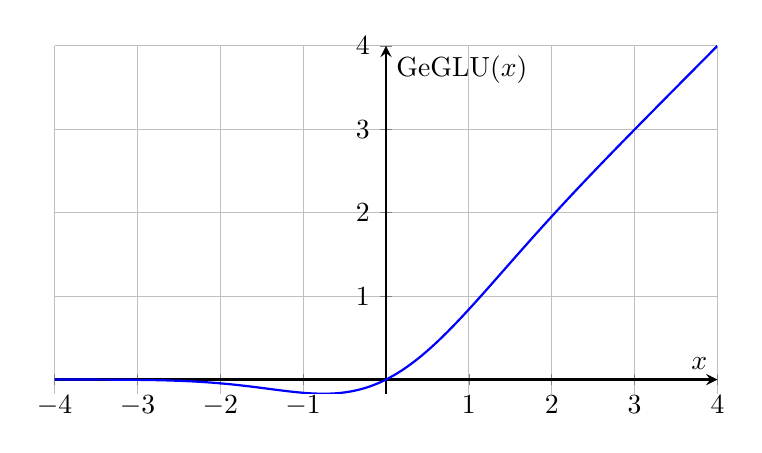
\begin{tikzpicture}
        \begin{axis}[
            axis lines = middle,
            xlabel = $x$,
            ylabel = {GeGLU$(x)$},
            samples = 200,
            domain = -4:4,
            width=10cm,
            height=6cm,
            grid = major,
            thick,
            smooth,
            legend pos=south east,
        ]
            \addplot [blue] {x * 0.5 * (1 + tanh(sqrt(2/pi)*(x + 0.044715 * x^3)))};
        \end{axis}
    \end{tikzpicture}
    \caption{Représentation de la fonction GeGLU basée sur l’approximation de GELU}
    \label{fig:geglu_plot}
    \end{figure}

    \item Alternance d'attention globale et locale : les couches d'attention locale utilisent des fen\^etres de 128 tokens avec RoPE $\theta = 10{,}000$, les couches globales ont une rotation plus lente $\theta = 160{,}000$ pour capturer les dépendances longues. Plus précisément, les couches d'attention de ModernBERT sont organisées selon un motif où deux couches consécutives utilisent une attention locale, suivies d'une couche à attention globale. L'attention locale dans ces couches, chaque token n'assiste qu'à une fenêtre glissante centrée autour de lui. Par défaut, cette fenêtre est de taille 128 tokens. Concrètement, pour un token de position $i$, seuls les tokens $j$ tels que $|i - j| \leq 64$ sont pris en compte dans le calcul d'attention. Cela réduit la complexité de l'attention de $\mathcal{O}(n^2)$ à $\mathcal{O}(n w)$ où $w$ est la taille de la fenêtre (ici 128). Cette attention locale est enrichie par RoPE avec $\theta = 10{,}000$, adapté aux échelles courtes. Toutes les positions s'attendent mutuellement. Elle est appliquée toutes les trois couches, et utilise une version lente de RoPE ($\theta = 160{,}000$), permettant de capturer des dépendances sémantiques distantes.

    \item Unpadding complet : avant calcul de l'attention, les tokens de padding sont supprimés, réduisant la complexité effective du traitement.

    \item FlashAttention est une méthode d'implémentation de l'attention softmax qui permet un calcul exact en mémoire optimisée, exploitant la parallélisation matérielle des GPU modernes (Tensor Cores, CUDA pipelines). Contrairement à l'implémentation naïve qui calcule puis stocke toute la matrice $QK^\top$, FlashAttention découpe le calcul en blocs (\textit{tiling}) afin de minimiser les accès mémoire et d'éviter l'écriture de matrices intermédiaires en RAM. La version utilisée dans ModernBERT (FlashAttention-2 ou 3 selon le backend). Il permet une exactitude numérique garantie à une précision de $10^{-5}$ par calcul de softmax à somme compensée. Le calcul est fait directement pendant l'accumulation des blocs, réduisant la consommation mémoire à $\mathcal{O}(n d)$ au lieu de $\mathcal{O}(n^2)$ pour la matrice d'attention. Tri par longueur des séquences dans un batch, permettant un groupement efficace des tokens valides dans les buffers CUDA, ce qui améliore la coalescence mémoire. Aussi, il est compatible avec les optimisations comme l'	extit{unpadding}, le RoPE et l'attention locale/globale, ce qui le rend idéal pour des encodeurs long-contexte comme ModernBERT.
\end{itemize}

Le pré-entraînement de ce nouveau modèle repose uniquement sur le MLM, sans NSP, mais avec un taux de masquage à 30\%. Également, il y a une tokenisation BPE inspirée d'OLMo, avec 83 tokens spécifiques et une taille de vocabulaire de 50,368. L'Optimiseur StableAdamW avec warmup de 2\% et décroissance linéaire. Afin il y a un Packing dynamique des séquences pour maintenir un batch GPU dense et stable.\\

Deux configurations de modèles sont proposés dans le papier :
\begin{itemize}
    \item ModernBERT-base : 22 couches, 768 dimensions, 149M param\`etres
    \item ModernBERT-large : 28 couches, 1024 dimensions, 395M param\`etres
    \item Contexte maximal : 8192 tokens
\end{itemize}

\newpage

Les résultats empiriques en \autoref{fig:pareto-modernbert} démontrent l'optimisation de Pareto de ModernBERT : 

\begin{figure}[H]
    \centering
    \includegraphics[width=0.9\linewidth]{images/modernbert_pareto_curve.png}
    \caption{Comparaison de l'efficience de Pareto Runtime vs GLUE}
    \label{fig:pareto-modernbert}
\end{figure}

Concernant les principales métriques de ModernBERT, le papier montre que pour GLUE benchmark surpasse DeBERTaV3-base tout en utilisant uniquement du MLM. Concernant BEIR / MLDR, il y a une meilleure précision en retrieval dense (BM25+encoder) et multi-vectoriel (ColBERT). Pour Code understanding, SOTA sur CodeSearchNet et StackQA, grâce à la présence de code dans le corpus de 2T tokens. Enfin, pour l'efficacité il y a jusqu'à 2$\times$ de rapidité que DeBERTaV3 pour des entrées longues. ModernBERT op\`ere asini une synth\`ese intelligente entre le paradigme LLM moderne et les besoins classiques de l'encodage, tout en conservant un design modulaire, open-source, et utilisable directement pour des cas d'usage industriels en retrieval, RAG ou classification.\\

L'architecture Transformer a fait évolué le champ du traitement automatique du langage, en remplaçant les mécanismes séquentiels classiques par une attention auto-référente efficace et massivement parallélisable. La première sous-section a détaillé les composants fondamentaux du modèle Transformer, en insistant sur le rôle  de la self-attention, des embeddings positionnels et du mécanisme multi-head, avant de présenter l’agencement général encodeur/décodeur. Ensuite, l’attention a été portée sur les architectures dérivées centrées sur l’encodage profond, avec en particulier BERT et ModernBERT, deux variantes qui illustrent l’évolution des modèles vers plus de profondeur. Toutefois, les Transformers présentent certaines limitations, notamment en ce qui concerne leur complexité quadratique en longueur de séquence, leur capacité à capturer des dépendances locales de manière efficace, ou encore leur intégration dans des systèmes contraints en ressources. Pour répondre à ces défis, de nouvelles architectures ont été proposées, mêlant modélisation continue, principes de l’espace d’état linéaire et efficience temporelle. L’une des plus prometteuses de cette nouvelle génération est l’architecture Mamba publié pour la première fois fin 2023.

\section{Architecture Mamba}

L’architecture Mamba s’inscrit dans une nouvelle génération de modèles séquentiels, conçus pour traiter efficacement des entrées de grande longueur tout en surmontant les limitations structurelles des architectures traditionnelles. Elle repose sur une intégration novatrice entre les mathématiques des \textit{State Space Models}, issus du contrôle et des systèmes dynamiques linéaires, et la flexibilité expressive des réseaux neuronaux profonds. En proposant une alternative aux Transformers, Mamba conserve une complexité temporelle linéaire,  tout en introduisant un mécanisme de sélection contextuelle, permettant une adaptation dynamique du modèle en fonction du contenu local des entrées pour la modélisation de longues séquences.\\

Les fondements théoriques de Mamba sont d'abord présentés, à travers une analyse des modèles linéaires à espace d’état, de leur formulation continue, puis de leur discrétisation numérique pour un usage efficace en contexte discret. Ensuite, l’introduction du mécanisme de sélection est détaillée. Ce mécanisme sera replacé dans le cadre plus large de l’architecture complète de Mamba, en lien avec les blocs MLP modernes et les réseaux récurrents. Mamba-2 est ensuite exposée. Ce dernier formalise une dualité structurée entre les SSMs et l’attention quadratique causale, permettant d’exploiter les deux modes de traitement dans un cadre unifié, plus efficace et plus parallèle. Enfin,  le modèle est présenté Llamba, une déclinaison récente et optimisée de Mamba-2, spécifiquement conçue pour la distillation depuis de grands modèles Transformers (tels que Llama-3). Llamba illustre l'application industrielle de Mamba dans des contextes contraints, tout en maintenant des performances grâce à une architecture légère et rapide à l’inférence.

\subsection{Fondements de Mamba}

La compréhension de l’architecture Mamba nécessite, avant, une étude des bases mathématiques sur lesquelles elle s’appuie. Contrairement aux modèles à attention, Mamba hérite directement de la théorie des systèmes dynamiques linéaires, en particulier des modèles à espace d’état, largement utilisés en contrôle automatique et traitement du signal. Ces modèles offrent une structure pour décrire l’évolution temporelle d’un système en fonction de ses entrées, à travers des équations différentielles ou des équations de récurrence discrètes. Ainsi, sont d’abord rappelés les principes théoriques des SSMs, leur formulation continue, ainsi que les principales méthodes de discrétisation permettant leur implémentation en environnement numérique. Ces éléments permettent à Mamba d'avoir ses propres innovations. En particulier, l’architecture repose sur l’idée que les dynamiques internes du système ne doivent plus être invariantes dans le temps, mais au contraire \textit{sélectivement adaptatives}, conditionnées par le contenu des séquences d’entrée. Cette perspective marque une rupture avec les SSMs classiques, et prépare la transition vers les mécanismes dynamiques spécifiques à Mamba détaillés dans les sous-sections suivantes.

\subsubsection{Contexte théorique : séquences longues et modèles linéaires structurés}

L'architecture Mamba, introduite en 2023 par \citep{gu2023mamba}, constitue une avance significative dans le domaine de la modélisation des séquences longues. Elle s'inscrit dans un effort de recherche visant à surmonter les limitations bien connues des Transformers en matière de complexité computationnelle et de capacité de généralisation sur des séquences de grande longueur.\\

Les Transformers, depuis leur introduction par \citep{vaswani2017attention}, ont dominé la modélisation de séquences dans une grande variété de domaines, allant du traitement du langage naturel à la génomique en passant par la vision par ordinateur. Leur capacité à capturer les dépendances globales grâce au mécanisme d'attention en a fait l'architecture de référence. Toutefois, ce mécanisme implique une complexité en temps et en mémoire quadratique en la longueur de la séquence, soit \( \mathcal{O}(L^2) \). Cela devient coûteux pour des entrées longues, telles que des documents complets, des séquences d'ADN, ou des flux audio continus.\\

Pour réduire cette complexité, plusieurs lignes de recherche ont émergé. Certaines se sont concentrées sur des variantes de l'attention, en tentant d'en rendre le coût sous-linéaire ou linéaire, comme dans Linformer, Performer, Longformer, ou Hyena \citep{poli2023hyena}. D'autres approches, plus radicales, ont proposé de s'affranchir totalement de l'attention pour revenir à des modèles récurrents ou convolutifs, tout en les modernisant grâce à une structuration mathématique inspirée de la physique et du contrôle : les State Space Models.\\

Les SSM structurés, popularisés par le modèle \textbf{S4} \citep{sun2023retnet}, offrent une alternative intéressante en modélisant une dynamique linéaire dans un espace latent, contrôlée par les entrées. Leur grande force réside dans leur complexité linéaire en la taille de la séquence, tout en permettant des calculs parallélisables via des convolutions efficaces. Ces modèles se sont montrés prometteurs sur des données audio, séquentielles continues, et génomiques.\\

Cependant, une limitation persistante des SSMs classiques est leur invariance temporelle : les paramètres gouvernant l'évolution de l'état latent (tels que les matrices de transition et les vecteurs d'entrée) sont fixes dans le temps. Cela rend ces modèles peu adaptatifs, notamment dans des contextes où l'information à mémoriser ou à ignorer varie en fonction du contenu. En d'autres termes, ils sont incapables de \textit{sélectionner dynamiquement} les informations pertinentes à conserver ou à oublier.\\

C'est cette limitation que Mamba cherche à lever. En introduisant le concept de Selective State Space Models, Mamba déforme le cadre traditionnel des SSMs pour permettre une dépendance explicite du contenu des entrées dans les dynamiques internes du modèle. Concrètement, les paramètres du modèle (tels que le vecteur de mise à jour de l'état ou le vecteur de sortie) deviennent eux-mêmes des fonctions non-linéaires des entrées. Cela permet une forme de sélection contextuelle, où le modèle apprend à filtrer, mettre en pause ou mettre à jour l'information en fonction du contenu local.\\

Ce changement de paradigme est profond : Mamba conserve les avantages d'efficacité des SSMs, mais acquiert la flexibilité fonctionnelle des architectures à attention. Pour y parvenir sans explosion de coûts mémoires, les auteurs conçoivent un algorithme de scan efficace sur GPU, qui simule le passage récursif à travers les états sans matérialiser l'ensemble de la trajectoire. Cette implémentation hautement optimisée permet à Mamba d'atteindre une vitesse d'inférence comparable à celle des RNNs tout en surpassant les Transformers sur plusieurs benchmarks, y compris sur des données textuelles, audio ou biologiques.\\

Cette première mise en contexte a permis de souligner les défis posés par les longues séquences ainsi que les limitations des architectures existantes, notamment l'invariance temporelle des modèles à espace d’état classiques. Pour mieux comprendre les fondements de Mamba et sa capacité à surmonter ces obstacles, il convient à présent de présenter les State Space Models avec leur formulation continue et discrète.

\subsubsection{State Space Models (SSM)}

Les modèles à espace d’état (State Space Models, ou SSM) constituent une classe puissante de modèles mathématiques largement utilisée dans les domaines du contrôle optimal, du traitement du signal et plus récemment de la modélisation de séquences longues. Leur formalisme repose sur la décomposition d’un système dynamique linéaire en deux équations fondamentales : une équation d’état et une équation d’observation.\\

La version continue d’un SSM linéaire temporellement invariant (LTI) est donnée par le système d’équations différentielles suivant :

\begin{equation}
\begin{cases}
\frac{d}{dt} h(t) = A h(t) + B u(t) \\
\quad y(t) = C h(t)
\end{cases}
\label{eq:ssm_continu}
\end{equation}

avec :
\begin{itemize}
    \item $h(t) \in \mathbb{R}^N$ : vecteur d'état caché à l'instant $t$,
    \item $u(t) \in \mathbb{R}^d$ : entrée externe (input),
    \item $y(t) \in \mathbb{R}^d$ : sortie observée,
    \item $A \in \mathbb{R}^{N \times N}$ : matrice de transition,
    \item $B \in \mathbb{R}^{N \times d}$ : matrice de contrôle,
    \item $C \in \mathbb{R}^{d \times N}$ : matrice d'observation.
\end{itemize}

Une méthode classique pour discrétiser le système continu \eqref{eq:ssm_continu} est le schéma d’intégration du trapèze, à mi-chemin entre les points $t$ et $t+1$. Elle est aussi connue comme la méthode bilinéaire ou Tustin. Il faut intégrer l’équation d’état sur l’intervalle $[t, t+\Delta]$ :

\begin{equation}
    h(t+\Delta) = h(t) + \int_t^{t+\Delta} \left( A h(s) + B u(s) \right) ds
\end{equation}

En appliquant la règle du trapèze, il est approximé l'intégrale par :
\begin{equation}
    h(t+\Delta) \approx h(t) + \frac{\Delta}{2} \left[ (A h(t) + B u(t)) + (A h(t+\Delta) + B u(t+\Delta)) \right]
\end{equation}

En regroupant les termes :
\begin{align*}
    h(t+\Delta) - \frac{\Delta}{2} A h(t+\Delta) &\approx h(t) + \frac{\Delta}{2} A h(t) + \frac{\Delta}{2} B \left( u(t) + u(t+\Delta) \right) \\
    \left( I - \frac{\Delta}{2} A \right) h(t+\Delta) &\approx \left( I + \frac{\Delta}{2} A \right) h(t) + \Delta B u_{\text{avg}}(t)
\end{align*}

avec $u_{\text{avg}}(t) = \frac{1}{2}(u(t) + u(t+\Delta))$. En posant :
\begin{equation}
\bar{A} = \left( I - \frac{\Delta}{2} A \right)^{-1} \left( I + \frac{\Delta}{2} A \right), \quad
\bar{B} = \left( I - \frac{\Delta}{2} A \right)^{-1} \Delta B
\end{equation}

ainsi la dynamique discrète :
\begin{equation}
    h_{t+1} = \bar{A} h_t + \bar{B} u_{\text{avg}}(t)
\end{equation}

Cette méthode garantit une bonne stabilité numérique, et est souvent utilisée dans les implémentations SSM modernes à cause de sa précision accrue par rapport à la méthode d’Euler explicite. La sortie observée reste :

\begin{equation}
    y_t = C h_t
\end{equation}

Cette récurrence peut s’écrire sous la forme d’une convolution. Pour cela, il suffit d’itérer les équations du système :

\begin{equation}
    x_k = \bar{A} x_{k-1} + \bar{B} u_k, \quad y_k = \bar{C} x_k
\end{equation}

Commençons par la première ligne du système :

étape 0 :
\begin{equation*}
    x_0 = \bar{B} u_0
\end{equation*}

étape 1 :
\begin{equation*}
    x_1 = \bar{A} x_0 + \bar{B} u_1 = \bar{A} \bar{B} u_0 + \bar{B} u_1
\end{equation*}

étape 2 :
\begin{equation*}
    x_2 = \bar{A} x_1 + \bar{B} u_2 = \bar{A}^2 \bar{B} u_0 + \bar{A} \bar{B} u_1 + \bar{B} u_2
\end{equation*}

Il est possible de constater que $x_k$ peut s’écrire comme une combinaison linéaire pondérée des entrées $u_0, \dots, u_k$ par des puissances successives de $\bar{A}$. Passant ensuite à la seconde ligne du système, où il est injecté les $x_k$ :

étape 0 :
\begin{equation*}
    y_0 = \bar{C} x_0 = \bar{C} \bar{B} u_0
\end{equation*}

étape 1 :
\begin{equation*}
    y_1 = \bar{C} x_1 = \bar{C} (\bar{A} \bar{B} u_0 + \bar{B} u_1) = \bar{C} \bar{A} \bar{B} u_0 + \bar{C} \bar{B} u_1
\end{equation*}

étape 2 :
\begin{equation*}
    y_2 = \bar{C} x_2 = \bar{C} (\bar{A}^2 \bar{B} u_0 + \bar{A} \bar{B} u_1 + \bar{B} u_2) = \bar{C} \bar{A}^2 \bar{B} u_0 + \bar{C} \bar{A} \bar{B} u_1 + \bar{C} \bar{B} u_2
\end{equation*}

Il est alors identifié un noyau de convolution discret :
\begin{equation}
    \bar{K}_k = (\bar{C}\bar{B}, \bar{C}\bar{A}\bar{B}, \dots, \bar{C}\bar{A}^k\bar{B})
\end{equation}

La sortie $y_k$ est donc donnée par :
\begin{equation}
    y_k = \sum_{\tau=0}^k \bar{K}_{k - \tau} u_{\tau} = (\bar{K} * u)_k
\end{equation}

Cette forme convolutionnelle est la base des implémentations rapides par transformée de Fourier (FFT) dans les SSMs modernes. Cette observation est essentielle pour l'implémentation efficace des SSMs : plut\^ot que de simuler les états $h_t$ un par un (récurrence lente), on peut calculer la sortie par convolution FFT avec le noyau $K$, ce qui permet un parallélisme GPU maximal.\\

Toutefois dans \citep{gu2021combining}, les auteurs démontrent que la méthode de discrétisation ZOH permet d'obtenir un meilleur résultat : 

\begin{equation}
    \frac{d}{dt} h(t) = A h(t) + B u(t), \quad y(t) = C h(t)
\end{equation}

Le but de la discrétisation par la méthode ZOH est d’obtenir une version discrète à pas fixe $\Delta$ de ce système. On suppose que l’entrée $u(t)$ est constante sur chaque intervalle $[k\Delta, (k+1)\Delta)$. La solution analytique de l'équation différentielle linéaire est :

\begin{equation}
    h(t + \Delta) = e^{A \Delta} h(t) + \int_0^\Delta e^{A (\Delta - \tau)} B u(t) \, d\tau
\end{equation}

Sous l’hypothèse ZOH ($u(t+\tau) = u(t)$ pour $\tau \in [0, \Delta]$), cela devient :

\begin{equation}
    h_{k+1} = e^{A \Delta} h_k + \left( \int_0^\Delta e^{A (\Delta - \tau)} \, d\tau \right) B u_k
\end{equation}
Or,
\begin{equation}
    \int_0^\Delta e^{A (\Delta - \tau)} d\tau = \left( \int_0^\Delta e^{A s} ds \right) = A^{-1} (e^{A \Delta} - I)
\end{equation}

(en supposant $A$ inversible).\\

D'où la forme discrète du système :
\begin{align}
    \bar{A} &= e^{A \Delta} \\
    \bar{B} &= (e^{A \Delta} - I) A^{-1} B \\
    \bar{C} &= C
\end{align}

La dynamique discrète est donc :
\begin{equation}
    h_{k+1} = \bar{A} h_k + \bar{B} u_k, \quad y_k = \bar{C} h_k
\end{equation}

Cette méthode a l’avantage de préserver la structure exponentielle de la solution du système, ce qui est utile dans les modèles comme S4 ou Mamba où les SSMs sont appliqués à des séquences temporelles longues.\\

Dans le cas d’un modèle à une dimension ($A = -\lambda$ scalaire, $B = 1$), il est obtenu : 
\begin{equation}
    \bar{A} = e^{-\lambda \Delta}, \quad \bar{B} = (1 - e^{-\lambda \Delta}) / \lambda
\end{equation}

Pour résumé il est obtenu avec les deux méthodes : 

\begin{table}[H]
\centering
\sffamily
\renewcommand{\arraystretch}{1.8}
\begin{tabular}{|c|c|c|}
\hline
\textbf{Discrétisation} & \textbf{Bilinéaire} & \textbf{ZOH} \\
\hline
\multirow{}{}{\textbf{Récurrence}} &
$\bar{A} = \left(I - \frac{\Delta}{2} A\right)^{-1}\left(I + \frac{\Delta}{2} A\right)$ &
$\bar{A} = e^{A\Delta}$ \\
& $\bar{B} = \left(I - \frac{\Delta}{2} A\right)^{-1} \Delta B$ &
$\bar{B} = (\bar{A} - I) A^{-1} B$ \\
& $\bar{C} = C$ & $\bar{C} = C$ \\
\hline
\textbf{Convolution} & $\bar{K}_k = (\bar{C}\bar{B}, \bar{C}\bar{A}\bar{B}, \dots, \bar{C}\bar{A}^k\bar{B})$ & $\bar{K} = \left( C e^{A\cdot k\Delta}(e^{A\Delta} - I)A^{-1}B \right)_{0 \leq k < L}$ \\
\hline
\end{tabular}
\caption{Discrétisation des équations d'état et expression du noyau de convolution}
\end{table}

Pour la ZOH, après avoir déroulé les calculs, on obtient en fin de compte :

\begin{equation}
    y_k = \sum_{j=0}^k \bar{C} \bar{A}^j \bar{B} u_{k-j} = \sum_{j=0}^k \bar{K}_j u_{k-j}
\end{equation}

Ce noyau peut \^etre précalculé ou appris de manière efficace, et est essentiel pour la parallélisation des calculs dans les SSMs modernes.\\

Dans le noyau de convolution développé plus haut, les coefficients $\bar{C}$ et $\bar{B}$ peuvent \^etre considérés comme des scalaires (ou vecteurs) apprenables. Concernant la matrice $\bar{A}$, il a été vu qu'elle intervient à la puissance $k$ au temps $k$, ce qui peut devenir co\^uteux en calcul pour des longues séquences. Une stratégie classique pour rendre les puissances de $\bar{A}$ faciles à calculer est de supposer que $\bar{A}$ est diagonale :

\begin{equation}
A = \begin{bmatrix}
\lambda_1 & 0 & \cdots & 0 \\
0 & \lambda_2 & \cdots & 0 \\
\vdots & \vdots & \ddots & \vdots \\
0 & 0 & \cdots & \lambda_n
\end{bmatrix} \Rightarrow A^k = \begin{bmatrix}
\lambda_1^k & 0 & \cdots & 0 \\
0 & \lambda_2^k & \cdots & 0 \\
\vdots & \vdots & \ddots & \vdots \\
0 & 0 & \cdots & \lambda_n^k
\end{bmatrix}
\end{equation}

Par le théorème spectral de l’algèbre linéaire, cela correspond à une classe de matrices dites normales. En pratique, le choix de la discrétisation (Euler, trapèze, etc.) et de l’initialisation de $\bar{A}$ joue un rôle crucial dans les performances du modèle. Il a été observé empiriquement que des matrices $A$ aléatoires donnent de très mauvais résultats, tandis qu’une initialisation issue de la matrice HiPPO (High-Order Polynomial Projection Operator) conduit à une nette amélioration (de 60 \% à 98\% de précision sur MNIST seq.).\\

La matrice HiPPO a été introduite dans \citep{gu2020hippo} puis reprise dans les modèles S4 \citep{sun2023retnet} et LSSL. Elle prend la forme suivante :

\begin{equation}
A_{nk} = \begin{cases}
(-1)^{n-k} (2k+1), & n > k \\
k + 1, & n = k \\
0, & n < k
\end{cases}
\end{equation}

Cette matrice n’est pas diagonale, ni même normale, mais elle peut être décomposée comme la somme d’une matrice normale et d’une matrice de rang faible, connue sous le nom de décomposition NPLR (Normal Plus Low Rank) :

\begin{equation}
A = V \Lambda V^{-1} + P Q^T
\end{equation}

La matrice $A$ peut être approchée par une matrice diagonalisable $A_0 = V \Lambda V^{-1}$, où $\Lambda$ est une matrice diagonale contenant les valeurs propres dominantes de $A$, et $V$ la base propre associée (approximative ou exacte). L’écart entre $A$ et $A_0$ est capturé par un terme $A - A_0 = P Q^T$, où $P$ et $Q$ sont de faible rang. Cela revient à dire que l’information non diagonalisable de $A$ est contenue dans une perturbation à faible rang. Ainsi, la structure $A = V \Lambda V^{-1} + P Q^T$ capture le comportement principal de $A$ via $\Lambda$ (facile à exponentier) et sa complexité contextuelle par $P Q^T$.\\

Les auteurs de S4 montrent que cette classe de matrices peut être exploitée efficacement par trois techniques algorithmiques : série génératrice tronquée, noyaux de Cauchy, et identité de Woodbury (cf. Algorithme 1 \autoref{fig:ssm-s4}). Les détails de la preuve montrant qu’une matrice NPLR peut être utilisée comme une matrice diagonale à coût efficace figurent dans les appendices B et C du papier \citep{sun2023retnet}. Dans une suite de travaux intitulée How to Train Your HiPPO \citep{gu2022trainhippo}, les auteurs ont affiné la manière de construire et d’initialiser la matrice HiPPO, donnant naissance à une version mise à jour du modèle connue sous les noms de S4 V2 ou S4 Updated, à opposer à S4 Original. Enfin, certains auteurs comme Ankit Gupta ont proposé d’utiliser directement une matrice diagonale apprise (plutôt qu’une structure NPLR), une approche aujourd’hui largement adoptée pour sa simplicité d’implémentation et ses bonnes performances pratiques.\\

Malgré leur efficacité, les SSMs LTI souffrent de plusieurs limitations. D’abord, l’invariance temporelle empêche l’adaptation dynamique aux entrées. Ensuite, le filtre convolutionnel $K$ est fixe pour toutes les entrées. Enfin, ils n’ont pas de mécanisme explicite de sélection contextuelle. C’est dans ce contexte que s’inscrit l’architecture Mamba, qui propose de lever ces limitations tout en conservant les avantages structurels des SSMs par un mécanisme de sélection.

\subsubsection{Mécanisme de sélection dans les SSMs}

Dans les modèles à espace d’état linéaire traditionnels, la dynamique est régie par des matrices fixes :
\begin{equation}
    h_t = \bar{A} h_{t-1} + \bar{B} x_t, \quad y_t = \bar{C} h_t
\end{equation}
Ces paramètres (\(\bar{A}, \bar{B}, \bar{C}\)) sont typiquement issus de la discrétisation d’un système linéaire continu, via une méthode comme le schéma bilinéaire ou ZOH, et restent invariants au cours du temps. Toutefois, un tel système ne peut pas s’adapter dynamiquement au contenu des entrées. Pour y remédier, le mécanisme de sélection introduit par Mamba permet de moduler dynamiquement le comportement du système à chaque pas de temps, en rendant le pas de temps \(\Delta_t\) dépendant de l’entrée \(x_t\).\\

Le mécanisme de sélection repose sur la modulation de la dynamique via un paramètre $\Delta_t$ appris conditionnellement à l’entrée :
\begin{equation}
    \Delta_t = \tau_\Delta (\text{Param} + s_\Delta(x_t))
\end{equation}
avec :
\begin{itemize}
    \item $\tau_\Delta$ : fonction d’activation positive et différentiable (par exemple softplus ou exp)
    \item $s_\Delta$ : projection linéaire (MLP ou Linear) de l’entrée $x_t$
\end{itemize}

Ce paramètre $\Delta_t$ est ensuite utilisé pour discrétiser le SSM de façon dynamique :
\begin{equation}
    \bar{A}_t, \bar{B}_t = \texttt{discretize}(\Delta_t, A, B)
\end{equation}

La récurrence devient alors :
\begin{equation}
    h_t = \bar{A}_t h_{t-1} + \bar{B}_t x_t, \quad y_t = \bar{C}_t h_t
\end{equation}

Le modèle peut choisir d’oublier ou de propager certaines entrées selon leur contenu. Il permet également de faire le lien entre les dynamiques discrètes récurrentes et continues. La sélection est continue et permet l’entraînement via gradient. Ce mécanisme est important dans l’architecture Mamba, où il est appliqué au niveau de la couche SSM pour permettre un traitement adaptatif et efficace des séquences longues.

\begin{figure}[H]
\centering
\includegraphics[scale=0.5]{images/algos_ssm_S4.png}
\caption{Algorithmes SSM S4 et SSM + Selection (S6)}
\label{fig:ssm-s4}
\end{figure}

La \autoref{fig:ssm-s4} compare l’implémentation classique (S4) avec celle enrichie du mécanisme de sélection (Mamba), en montrant l’évolution vers une dynamique dépendante du contenu, étape par étape.\\

Le mécanisme de sélection, en permettant de moduler dynamiquement les coefficients du modèle en fonction du contenu des entrées, constitue le cœur de l’innovation introduite par Mamba. Dans la section suivante, sera présentée l’architecture complète de Mamba, qui intègre ce mécanisme au sein d’un bloc modulaire, combinant efficacement transformations linéaires, non-linéarités, et traitement séquentiel parallèle. Cette architecture s’inscrit dans la continuité des RNNs modernes tout en introduisant des éléments conceptuellement proches des MLPs profonds.

\subsubsection{Architecture Mamba}

Le mécanisme de sélection introduit dans Mamba peut être interprété comme une généralisation des mécanismes de porte classiques des RNNs. Il a été observé que les portes des RNNs sont liées à la discrétisation de systèmes dynamiques en temps continu, une idée bien établie dans la littérature (voir \citep{funahashi1993approximation}, \citep{tallec2018can}). Dans cette optique, le paramètre $\Delta$ utilisé dans les SSMs s’interprète comme jouant un rôle généralisé des coefficients de porte des RNNs. Cette perspective permet d’établir un lien conceptuel entre les mécanismes heuristiques de porte et les fondations mathématiques rigoureuses des SSMs discrétisés. Ce lien est formalisé par le résultat au théorème 2.2.

\newpage

\begin{theorem}
Lorsque \( N = 1 \), \( A = -1 \), \( B = 1 \), \( s_{\Delta} = \text{Linear}(x) \), et \( \tau_{\Delta} = \text{softplus} \), alors la récurrence du SSM sélectif (Algorithme 2) devient :
\begin{align}
    g_t &= \sigma(\text{Linear}(x_t)) \\
    h_t &= (1 - g_t) h_{t-1} + g_t x_t
\end{align}
\end{theorem}

Il s’agit ici d’une amélioration du lemme 3.1 de \citep{gu2021combining}, généralisée à la discrétisation ZOH et aux portes dépendantes de l’entrée. La preuve complète est fournie dans l’annexe C de l’article original. Cette formulation met en évidence l’utilisation de $s_{\Delta}$ comme transformation linéaire de l’entrée, et de $\tau_{\Delta}$ comme activation de type softplus pour obtenir un coefficient $\Delta_t$ positif et différentiable. En particulier, lorsqu’une entrée $x_t$ doit être totalement ignorée — comme c’est le cas dans certaines tâches synthétiques — il est nécessaire que tous les canaux $D$ l’ignorent. Pour cela, il est proposé de projeter $x_t$ sur une dimension scalaire, puis de répéter cette valeur sur les $D$ canaux via une diffusion (broadcasting).\\

L’architecture d’un bloc Mamba peut s’interpréter comme une généralisation unifiée des blocs H3 et des MLPs à portes (Gated MLPs). Comme présenté en \autoref{fig:bloc-mamba}.

\begin{figure}[H]
    \centering
    \includegraphics[width=1.0\linewidth]{images/mamba_architecture.png}
    \caption{\justifying Conception simplifiée de bloc combine le bloc H3 — qui constitue la base de la plupart des architectures à espace d’état — avec le bloc MLP, omniprésent dans les réseaux de neurones modernes. Au lieu d’alterner entre ces deux types de blocs, il est répété simplement le bloc Mamba de manière homogène. Par rapport au bloc H3, Mamba remplace la première porte multiplicative par une fonction d’activation. Par rapport au bloc MLP, Mamba ajoute un SSM (State Space Model) dans la branche principale. Pour la fonction d’activation $\sigma$, on utilise SiLU / Swish.}
    \label{fig:bloc-mamba}
\end{figure}

Elle intègre un SSM (State Space Model) comme transformation séquentielle principale, combiné à des projections linéaires et activations adaptatives. Premièrement, le Bloc H3 comporte deux branches parallèles (Conv et SSM), dont les sorties sont multipliées (gating). Ensuite, le Gated MLP structure purement MLP avec un produit entre une projection linéaire et une activation $\sigma$ de l’entrée (souvent SiLU). Pour finir, Mamba remplace le premier produit de H3 par une activation non-linéaire, et insère un SSM après une convolution. Le signal est donc filtré par la convolution, activé, puis intégré dynamiquement par le SSM. Le résultat est ensuite modulé par une autre activation. Le bloc Mamba applique donc les étapes suivantes :
\begin{enumerate}
    \item Deux projections linéaires en entrée (via Conv1D)
    \item Une branche passe dans un SSM (avec discrétisation adaptative)
    \item L’autre est activée via une fonction $\sigma$ (typiquement SiLU/Swish)
    \item Le produit à la sortie constitue l’output du bloc (gate multiplicatif)
\end{enumerate}

Ainsi, Mamba combine la structure hiérarchique (Conv + SSM) avec un mécanisme de sélection adaptatif (via $\Delta$) et la simplicité des blocs MLP modernes. Le tout forme un bloc homogène, empilé de manière répétée comme dans un Transformer. Contrairement à l’attention, le traitement est linéaire en la longueur de la séquence.\\

Mamba donc repose sur une refondation théorique des modèles à espace d’état linéaire, enrichis par un mécanisme de sélection contextuelle qui permet une adaptation dynamique aux entrées, tout en conservant une efficacité computationnelle linéaire. Cette architecture unifie plusieurs idées issues des réseaux de neurones modernes en les ancrant dans une modélisation continue et discrétisée de façon stable. Cette synthèse permis à Mamba de surpasser les Transformers sur plusieurs benchmarks séquentiels, tout en s'exécutant plus rapidement en inférence. Toutefois, malgré ses performances prometteuses, certaines limitations subsistent, notamment en termes de parallélisation des passes avant (forward pass) et de compatibilité avec les mécanismes d’attention traditionnels. C’est dans ce contexte qu’intervient Mamba-2, une extension  qui introduit une dualité structurée entre les modèles à espace d’état et l’attention quadratique, tout en renforçant la capacité de traitement parallèle. 

\subsection{Mamba-2}

Mamba-2 constitue une réponse directe aux limites de Mamba. Il propose un cadre unifié en articulant les SSMs autour d’une structure matricielle semi-séparable permettant une dualité explicite entre récurrence et attention. Cette reformulation ouvre la voie à un traitement parallèle plus rapide, tout en conservant les avantages structurels des SSMs. L’architecture est repensée pour faciliter la parallélisation des blocs, réduire les coûts d’inférence, et intégrer des schémas multi-têtes plus expressifs. Il est d'abord exposé les principales différences entre Mamba et Mamba-2, tant du point de vue algorithmique que de l’architecture du bloc élémentaire. Il est ensuite introduit le cadre théorique de la Structured State-Space Duality (SSD), qui établit une équivalence mathématique entre certains SSMs et des mécanismes d’attention quadratique structurée. L’exploitation algorithmique des matrices semi-séparables est démontré. Pour finir, l’architecture du bloc Mamba-2 est détaillée pour finir plusieurs optimisations systèmes sont analysées, conçues pour tirer parti du matériel moderne (multi-GPU).

\subsubsection{Différences et évolutions par rapport à Mamba}

La version Mamba-2 \citep{dao2024mamba2} constitue une amélioration théorique, algorithmique et systémique significative par rapport à la première version de Mamba \citep{gu2023mamba}. Alors que Mamba exploitait des State Space Models sélectifs avec des paramètres temporellement variables ($A_t, B_t, C_t$), Mamba-2 repose sur une version affinée de ces SSM sélectifs, tout en les intégrant dans un cadre dualisé plus riche, appelé Structured State-Space Duality (SSD).\\

Mamba-2 montre que certains SSMs structurés sont mathématiquement équivalents à une classe d’attention quadratique à masque structuré, au travers d'une matrice semi-séparable (semiseparable matrix). Cela permet de bénéficier à la fois de la forme récurrente linéaire (entraînement efficace) et de la forme quadratique (computation matricielle parallélisable). Simplification structurelle de $A$. Dans Mamba-2, la matrice $A_t$ de la récurrence est réduite à une identité multipliée par un scalaire, ce qui abaisse les coûts de pré-traitement et permet des calculs plus efficaces sur GPU/TPU. Utilisation de dimensions de tête $P$ plus grandes. Contrairement à Mamba où $P = 1$, Mamba-2 adopte des têtes multiples analogues à celles des Transformers (typiquement $P = 64$ ou $128$), facilitant l’usage de multiplications matricielles. Bloc parallélisable. Les projections linéaires dépendantes des données (par exemple $s_B(x)$) sont désormais placées en début de bloc, ce qui autorise une parallélisation tensorielle (comme dans Megatron). Intégration de structures analogues aux têtes d’attention. Mamba-2 introduit la notion de Grouped-Value Attention (GVA), une analogie des têtes multi-values (MVA) pour SSMs, permettant des variations d’architecture plus riches.\\

Empiriquement, Mamba-2 pareto-domine les Transformers++ et Mamba original à taille comparable sur les tâches de modélisation de langage. Par exemple, un modèle Mamba-2 avec 2.7B de paramètres entraîné sur 300B tokens dépasse les performances de Mamba 2.8B, Pythia 2.8B et même Pythia 6.9B sur The Pile. Les gains de temps d'entraînement sont aussi significatifs : jusqu’à 8 fois plus rapide que Mamba avec l’algorithme SSD. Enfin, les lois de scaling à la Chinchilla sont aussi vérifiées pour Mamba-2, renforçant son potentiel comme fondation pour des modèles de grande taille. Il est donc nécessaire de démontrer cette équivalence mathématique entre SSD et attention quadratique.

\subsubsection{Structured State-Space Duality (SSD) et attention quadratique}

L'un des apports théoriques majeurs de Mamba-2 est l'introduction du cadre de la Structured SSD, qui unifie les représentations récurrentes (type SSM) avec les mécanismes d'attention structurée.\\

Le point de départ est le système à espace d'état linéaire sélectif discretisé, de la forme :
\begin{equation}
    h_t = \bar{A}_t h_{t-1} + \bar{B}_t x_t, \quad y_t = \bar{C}_t h_t
\end{equation}

En développant cette récurrence\footnote{Pour simplifier les écritures, dans la suite toutes les matrices sont considérées comme discrétisées : $\bar{A} = A, \bar{B}=B, \bar{C}=C$.} dans le temps (\textit{unrolling}), on peut exprimer $h_t$ par :

\begin{equation}
\begin{split}
    h_t &= A_t h_{t-1} + B_t x_t \\
        &= A_t (A_{t-1} h_{t-2} + B_{t-1} x_{t-1}) + B_t x_t \\
        &= A_t A_{t-1} h_{t-2} + A_t B_{t-1} x_{t-1} + B_t x_t \\
        &= \dots \\
        &= \left(\prod_{i=s+1}^{t} A_i\right) B_s x_s + \dots + B_t x_t
\end{split}
\end{equation}

Ainsi, en injectant dans $y_t = C_t h_t$, on obtient :
\begin{align}
    y_t &= C_t h_t = C_t \left( \sum_{s=1}^{t} \left( \prod_{i=s+1}^{t} A_i \right) B_s x_s \right) = \sum_{s=1}^t K_{t,s} x_s
\end{align}

où le noyau $K \in \mathbb{R}^{L \times L}$ est appelé noyau convolutif ou matrice de transfert temporelle :
\begin{equation}
    K_{t,s} := C_t \left(\prod_{i=s+1}^{t} A_i\right) B_s
\end{equation}

Lorsque les matrices $A_t$ sont diagonales (ou m\^eme scalaires, c'est-à-dire $A_t = \lambda_t I$), les produits matriciels successifs deviennent scalaires (ou diagonaux), ce qui permet de factoriser les termes :
\begin{equation}
    \prod_{i=s+1}^t A_i = \exp\left(\sum_{i=s+1}^t \ln A_i\right)
\end{equation}
Dans le cas scalaire, on peut donc poser :
\begin{align*}
    U_t &= C_t \prod_{i=1}^t A_i \\
    V_s^\top &= \left(\prod_{j=1}^s A_j^{-1}\right) B_s
\end{align*}
ce qui donne :
\begin{equation}
    K_{t,s} = U_t V_s^T \quad \text{pour } s < t, \quad \text{et } 0 \text{ sinon}
\end{equation}

Ce type de matrice $K$ est appelé matrice semi-séparable causale, et se note $K = \text{tril}(UV^\top)$. Cette forme est mathématiquement équivalente à une attention causale quadratique sans normalisation (type Softmax), où $U_t$ joue le r\^ole de requ\^ete ($q_t$) et $V_s$ celui de clé ($k_s$) :
\begin{equation}
    y_t = \sum_{s < t} q_t^T k_s x_s
\end{equation}
avec $q_t = U_t$, $k_s = V_s$. La dualité SSD décrit ainsi un pont théorique entre la récurrence linéaire des SSMs (traitement à faible mémoire et en ligne) et les architectures attentionnelles (accès aléatoire à la séquence, traitement parallélisé).

\subsubsection{Matrices semi-separables et algorithme SSD}

Les bénéfices du développement du cadre théorique SSD entre les SSMs, l’attention et les matrices structurées résident dans l’utilisation de ces connexions pour améliorer à la fois les modèles et les algorithmes. Il est démontré que plusieurs algorithmes permettant de calculer efficacement les modèles SSD peuvent être dérivés d’algorithmes existants pour la multiplication de matrices structurées. Le résultat principal, sur le plan computationnel, est un algorithme capable de combiner les deux modes de traitement dans les modèles SSD : le mode linéaire (récursif) et le mode quadratique (attention). Cet algorithme est aussi efficace que les SSMs classiques en termes de coût computationnel (avec une complexité linéaire en la longueur de la séquence), tout en étant aussi adapté au matériel (hardware-friendly) que l’attention, en reposant essentiellement sur des multiplications matricielles.\\

\begin{definition}
Une matrice $M \in \mathbb{R}^{T \times T}$ est dite \textbf{N-semi-séparable} si toute sous-matrice strictement triangulaire inférieure a un rang au plus $N$.
\end{definition}

\begin{theorem}
Une matrice $M$ est N-SSS si elle peut s’écrire sous la forme :
\begin{equation}
    M_{ji} = C_j^\top A_{j} A_{j-1} \cdots A_{i+1} B_i \quad \text{pour } j \geq i
\end{equation}
avec $A_t \in \mathbb{R}^{N \times N}$, $B_t, C_t \in \mathbb{R}^{N}$.
\end{theorem}

Sous la forme globale, 
\begin{equation}
    y = Mx = \sum_{s=0}^t C_t^\top A_{t} A_{t-1} \cdots A_{s+1} B_s x_s
\end{equation}

\begin{definition}[Cas spécial 1-semi séparable]
Dans ce cas, $A_t$ devient un scalaire $a_t$, et la matrice $M$ est donnée par :
\begin{equation}
    M_{ji} = \prod_{k=i+1}^{j} a_k \quad \text{(cumprod)}
\end{equation}
\end{definition}

Il est possible de diviser la séquence en $B = T/Q$ chunks qui sont des blocs de taille $Q$.

\begin{equation}
M =
\begin{bmatrix}
M^{(0,0)} & 0        & 0        & \cdots & 0 \\
M^{(1,0)} & M^{(1,1)} & 0        & \cdots & 0 \\
M^{(2,0)} & M^{(2,1)} & M^{(2,2)} & \cdots & 0 \\
\vdots    & \vdots    & \vdots    & \ddots & \vdots \\
M^{(B-1,0)} & M^{(B-1,1)} & M^{(B-1,2)} & \cdots & M^{(B-1,B-1)}
\end{bmatrix}
\end{equation}

Dans le développement, le Bloc Diagonal (Local : Input $\rightarrow$ Output) :
\begin{equation}
    M^{(j,j)} = \text{SSM}(A_{jQ:(j+1)Q},\ B_{jQ:(j+1)Q},\ C_{jQ:(j+1)Q})
\end{equation}

Les blocs diagonaux sont simples à traiter, car ils correspondent à des sous-problèmes auto-similaires de taille plus petite. Le bloc $j$-ième correspond au calcul de la sortie :
\[ 
\text{SSM}(A_R, B_R, C_R)(x_R)
\]
pour l'intervalle $R = jQ : (j + 1)Q = (jQ, jQ + 1, \ldots, jQ + Q - 1)$.\\


L'élément clé est que ce bloc peut être calculé avec n'importe quelle méthode souhaitée. En particulier, pour de petites tailles de chunk $Q$, ce sous-problème est plus efficacement résolu en utilisant la forme quadratique duale SMA. De plus, les chunks peuvent être calculés en parallèle. Ces sous-problèmes peuvent être interprétés comme : « quelle est la sortie par chunk en supposant que l'état initial (du chunk) est nul ». Autrement dit, pour le chunk $j$, il est calculé les sorties correctes en ne tenant compte que des entrées locales $x_{jQ : (j + 1)Q}$.\\

Le Bloc Hors-Diagonale (Low Rank : Inter-chunk) :
\begin{equation}
    M^{(j,i)} =
    \left[
    \begin{array}{c}
        C_{jQ}^\top A_{jQ:(i+1)Q-1} \\
        \vdots \\
        C_{(j+1)Q - 1}^\top A_{(j+1)Q - 1:(i+1)Q - 1}
    \end{array}
    \right]
    \cdot
    \left[
    \begin{array}{c}
        B_{iQ}^\top A_{iQ+1:(i+1)Q -1} \\
        \vdots \\
        B_{(i+1)Q - 1}^\top
    \end{array}
    \right]^\top
\end{equation}

Chaque bloc est de rang \( \leq N \). Par exemple, \autoref{fig:exemple_blocs}, pour \( T = 9 \) avec une décomposition en chunks de longueur \( Q = 3 \). Les cellules ombrées représentent les factorisations de rang faible des blocs hors-diagonaux de la matrice semi-séparable.

\begin{figure}[H]
    \centering
    \includegraphics[width=1.0\linewidth]{images/matrices_semi_separables.png}
    \caption{\( T = 9 \) avec une décomposition en chunks de longueur \( Q = 3 \)}
    \label{fig:exemple_blocs}
\end{figure}

Il est possible à partir de cette structure de décomposer le problème en deux parties. Cela revient à diviser la sortie d’un chunk \( y_{jQ:(j+1)Q} \) en deux composantes :  
\begin{itemize}
    \item l’effet des entrées dans le chunk, soit \( x_{jQ:(j+1)Q} \) ;
    \item l’effet des entrées précédentes au chunk, soit \( x_{0:jQ} \).
\end{itemize}

La factorisation de rang faible consiste en trois termes, et il y a donc trois composantes distinctes dans le calcul associé. Dans cette factorisation, on utilise la terminologie suivante :

\begin{itemize}
    \item Les termes de la forme :
    \[
    \begin{bmatrix}
    B_0^\top A_{2:0} \\
    B_1^\top A_{2:1} \\
    B_2^\top A_{2:2}
    \end{bmatrix}
    \]
    sont appelés les facteurs droits ou blocs-$B$ (\emph{right factors} ou \emph{$B$-block-factors}). Cette étape consiste à effectuer la multiplication par les blocs-$B$ (facteurs droits) de la factorisation de rang faible. Pour chaque chunk, il s'agit d'une multiplication de matrice de taille $(N, Q)$ par $(Q, P)$, où $N$ est la dimension de l’état caché et $P$ est la dimension de la tête. Le résultat est un tenseur de dimension $(N, P)$ pour chaque chunk, ce qui correspond à l’état caché $h$ à l’issue du chunk. Cela peut s’interpréter comme : \og quel est l’état final produit par un chunk si l’on suppose que l’état initial de ce chunk est nul \fg. En d’autres termes, cela calcule $h_{jQ+Q-1}$ en supposant que $x_{0:jQ} = 0$.

    \item Les termes comme $A_{5:2}$ sont appelés les facteurs centraux ou blocs-$A$ (\emph{center factors} ou \emph{$A$-block-factors}). Cette étape calcule l’effet des blocs-$A$ (facteurs centraux) dans la factorisation de rang faible. À l’étape précédente, les états finaux de chaque chunk ont une forme globale de dimension $(T/Q, N, P)$. Ils sont multipliés maintenant par une matrice 1-SS construite à partir de :
    \[
    A_{2Q-1:Q-1},\ A_{3Q-1:2-Q-1},\ \dots,\ A_{T-1:T-Q-1}
    \]
    Cette étape peut être réalisée avec n’importe quel algorithme de multiplication de matrice 1-SS (à savoir, l’opérateur scan scalaire SSM ou \emph{cumprodsum}).
    \item Les termes de la forme :
    \[
    \begin{bmatrix}
    C_6^\top A_{6:5} \\
    C_7^\top A_{7:5} \\
    C_8^\top A_{8:5}
    \end{bmatrix}
    \]
    sont appelés les facteurs gauches ou blocs-$C$ (\emph{left factors} ou \emph{$C$-block-factors}). Cette étape réalise la multiplication par les blocs-$C$ (facteurs gauches) dans la factorisation de rang faible. Pour chaque chunk, cette opération peut \^etre vue comme une contraction matricielle de type $\text{contract}(QN, NP \rightarrow QP)$. On peut l'interpréter comme suit : \og quelle est la sortie par chunk si l'on dispose du bon état initial $h_{jQ-1}$ et que les entrées locales $x_{jQ:(j+1)Q}$ sont nulles \fg. En d'autres termes, pour le chunk $j$, cela permet de calculer les sorties correctes en ne tenant compte que des entrées précédentes $x_{0:jQ}$.
\end{itemize}

\begin{figure}[H]
    \centering
    \includegraphics[width=1.0\linewidth]{images/sdd_algorithm.png}
    \caption{\justifying \textbf{(Algorithme SSD.)} En utilisant le point de vue transformation matricielle des modèles à espace d'état pour les réécrire sous forme de matrices semi-séparables, il est développé un calcul plus efficace matériellement du modèle SSD à travers un algorithme de multiplication matricielle par décomposition en blocs \citep{dao2024mamba2}.}
    \label{fig:ssd_algo}
\end{figure}

Cette multiplication matricielle présénté par l'algorithme SSD en \autoref{fig:ssd_algo} admet aussi une interprétation comme un modèle à espace d'état, où les blocs correspondent au découpage de la séquence d'entrée et de sortie en chunks. Les blocs diagonaux représentent les calculs intra-chunk, tandis que les blocs hors-diagonaux représentent les calculs inter-chunks, transmis via l'état caché du SSM. Concrètement, l'algorithme SSD décompose l'action du noyau convolutionnel temporel $K \in \mathbb{R}^{T \times T}$ en blocs diagonaux (intra-chunk) et hors-diagonaux (inter-chunk), où les blocs inter-chunks sont approximés par des produits de matrices de rang faible. Cette décomposition exploite la représentation semi-séparable des modèles SSM, pour lesquels la sortie $y_t$ peut s’écrire comme une somme pondérée des entrées passées selon la formule :

\begin{equation}
y_t = \sum_{s=1}^t K_{t,s} x_s = \sum_{s=1}^t C_t \left( \prod_{i=s+1}^{t} A_i \right) B_s x_s
\end{equation}

où les poids $K_{t,s}$ correspondent à une convolution causale générée par la dynamique linéaire du système. L’idée centrale de SSD est donc de transcrire cette relation récurrente en une forme matricielle factorisable, c’est-à-dire :

\begin{equation}
K = \mathrm{tril}(UV^\top)
\end{equation}

avec $\displaystyle U_t = C_t \prod_{i=1}^t A_i$ et $V_s^\top = \displaystyle \left( \prod_{j=1}^s A_j^{-1} \right) B_s$, ce qui correspond à une factorisation de rang faible causale.\\

L’algorithme SSD exploite donc cette factorisation en divisant la séquence en blocs temporels, puis en distinguant en les calculs locaux (intra-chunk), résolus via des SSM classiques sur une fenêtre glissante. Mais aussi par des les interactions longue portée (inter-chunk), traitées efficacement grâce à une factorisation de rang faible des contributions passées, via les matrices blocs-$A$, blocs-$B$, blocs-$C$.\\

Après avoir exposé le cadre théorique sous-jacent à l'algorithme SSD et sa mise en œuvre à travers les matrices semi-séparables, il est désormais possible d'en comprendre l'intégration concrète dans l'architecture Mamba-2, en particulier à travers la conception de ses blocs computationnels et les choix de factorisation mis en œuvre pour optimiser l'inférence et l'entraînement.

\subsubsection{Architecture Mamba-2}

Le bloc Mamba-2 est défini comme une simplification de l'architecture Mamba initiale. Les projections linéaires séquentielles y sont supprimées, ce qui réduit la complexité computationnelle. 

\begin{figure}[H]
    \centering
    \includegraphics[width=1\linewidth]{images/mamba-2_architecture.png}
    \caption{\justifying Les paramètres du SSM \( A, B, C \) sont directement générés en début de bloc, plutôt qu'en fonction de l'entrée \( X \), ce qui permet une parallélisation plus efficace et une réduction des délais d'inférence. De plus, une couche de normalisation supplémentaire, inspirée de NormFormer \cite{shleifer2021normformer}, est ajoutée pour améliorer la stabilité de l'entraînement. Enfin, les projections $B$ et $C$ utilisent une seule tête partagée entre les différentes têtes $\mathbf{X}$, de manière analogue à l'attention multi-valeurs (Multi-Value Attention, MVA) \citep{dao2024mamba2}.}
    \label{fig:enter-label}
\end{figure}

\paragraph{Projections de paramètres parallèles.} Dans Mamba-1, une vision centrée sur les SSM était adoptée, dans laquelle la couche SSM sélective était considérée comme une application $\mathbf{X} \mapsto Y$. Les paramètres SSM $A, B, C$ étaient alors considérés comme secondaires et définis comme des fonctions de l’entrée $\mathbf{X}$. Ainsi, les projections linéaires définissant $(A, B, C)$ étaient appliquées \emph{après} la projection linéaire initiale produisant $\mathbf{X}$.\\

Dans Mamba-2, la couche SSD est considérée comme une application $(A, X, B, C) \mapsto Y$. Il est donc jugé logique que $A, X, B, C$ soient produits en parallèle, à l’aide d’une seule projection au début du bloc. Cette approche est analogue aux architectures d’attention classiques, où $\mathbf{X}, B, C$ correspondent respectivement aux projections $Q, K, V$ qui sont générées simultanément.\\

L’adoption des projections parallèles pour les entrées $A, B, C, X$ du SSM permet une réduction modérée du nombre de paramètres, mais surtout, elle rend le modèle plus compatible avec le parallélisme tensoriel, en particulier dans le cadre de modèles de grande taille, selon les schémas de partitionnement proposés dans Megatron \citep{shoeybi2019megatron}.

\paragraph{Normalisation supplémentaire.}Lors d’expériences préliminaires, des instabilités ont été constatées dans les grands modèles. Ces instabilités ont pu être atténuées par l’ajout d’une couche de normalisation supplémentaire (comme LayerNorm, GroupNorm ou RMSNorm) juste avant la projection de sortie finale du bloc.\\

L’usage de cette normalisation s’inspire directement de l’architecture NormFormer \citep{shleifer2021normformer}, où des couches de normalisation sont également ajoutées à la fin des blocs MLP et MHA.\\

Il est également noté que cette modification est similaire à celles introduites dans d’autres modèles récents proches de Mamba-2, conçus selon une perspective d’attention linéaire. Dans les formulations d’attention linéaire d’origine, une normalisation est effectuée par un terme au dénominateur simulant celle de la fonction softmax utilisée dans l’attention classique. Les modèles TransNormerLLM \citep{qin2023transnormerllm} et RetNet \citep{sun2023retnet} ont montré que cette forme de normalisation pouvait induire de l’instabilité, ce qui a motivé l’ajout d’une couche LayerNorm ou GroupNorm supplémentaire après la couche d’attention linéaire.\\

La couche de normalisation supplémentaire proposée ici diffère légèrement : elle est placée après la branche de porte multiplicative (multiplicative gate), et non avant.

\paragraph{Schémas multi-têtes pour les transformations de séquence.} En rappelant  que les SSMs sont définis comme des transformations de séquence dans lesquelles :
\begin{itemize}
    \item les paramètres $A, B, C$ ont une dimension d'état $N$ ;
    \item ils définissent une transformation de séquence $\mathbb{R}^T \rightarrow \mathbb{R}^T$, qui peut par exemple être représentée par une matrice $M \in \mathbb{R}^{T \times T}$ ;
    \item cette transformation opère sur une séquence d'entrée $\mathbf{X} \in \mathbb{R}^{T \times P}$, indépendamment sur l'axe $P$.
\end{itemize}

\newpage

Cela peut être interprété comme la définition d'une seule tête de transformation de séquence.

\begin{definition}[Schémas multi-têtes] Une transformation de séquence multi-têtes est composée de $H$ têtes indépendantes, pour un modèle de dimension totale $D = d \cdot H$. Les paramètres peuvent être partagés entre les têtes, ce qui définit un schéma de têtes.
\end{definition}

La taille d'état $N$ et la dimension de tête $P$ sont respectivement analogues à la dimension des têtes $QK$ et à celle des têtes $V$ dans l'attention. De même que dans les architectures Transformer modernes \citep{chowdhery2023palm, touvron2023llama}, dans Mamba-2, ces dimensions sont généralement choisies comme des constantes (typiquement 64 ou 128). Lorsque la dimension du modèle $D$ augmente, le nombre de têtes est augmenté, tout en gardant les dimensions $N$ et $P$ constantes. Pour décrire cette stratégie, les idées issues de l'attention multi-têtes peuvent être transférées et généralisées afin de définir des schémas similaires pour les SSMs ou toute autre transformation de séquence générale :
\begin{itemize}
    \item MHS (Multihead SSM) : chaque tête est une copie indépendante du SSM avec ses propres paramètres $A, B, C$. Le nombre de têtes est $H = D / P$. Ce schéma est analogue à l'attention multi-têtes classique (MHA), mais généralisable à toute transformation de séquence.
    \item MCS (Multi-contract SSM) : les paramètres $B$ et $\mathbf{X}$ (analogues à $V$ et $K$ dans l'attention) sont partagés entre les têtes, tandis que $C$ est spécifique à chaque tête. Cela rappelle le schéma de l'attention multi-queries (MQA), connu pour accélérer l'inférence autoregressive \citep{shazeer2019multiquery}.
    \item MES (Multi-expand SSM) : $C$ et $\mathbf{X}$ sont partagés entre les têtes, mais $B$ est indépendant, ce qui permet une expansion différente des états cachés pour chaque tête (analogue à multi-key attention).
    \item MIS (Multi-input SSM) : ici, $\mathbf{X}$ est vu comme l’entrée principale du SSM, et $B$, $C$ sont partagés à travers tous les canaux. Ce schéma, appelé aussi MVA (multi-value attention), correspond à l’architecture de Mamba originale, où chaque canal d’entrée a sa propre dynamique $A$ mais partage les paramètres $B, C$.
\end{itemize}

\newpage

\begin{proposition} La couche SSM sélective (S6) dans l’architecture Mamba \citep{gu2023mamba} peut être interprétée ainsi comme une dimension de tête $P = 1$ : chaque canal possède une dynamique SSM indépendante définie par $A$. Lastructure de tête MIS (ou MVA) : les matrices $B$ et $C$ (équivalentes à $K$ et $Q$ dans l’attention) sont partagées entre tous les canaux d’entrée $\mathbf{X}$ (analogue à $V$).
\end{proposition}

Ces variantes de schémas de tête peuvent être ablatées dans les SSD. Malgré un contrôle strict du nombre de paramètres et de la dimension d’état totale, des différences notables de performance sont observées en aval. Il a été empiriquement constaté que le schéma MVA utilisé dans Mamba donne les meilleurs résultats.\\

Au-delà des innovations architecturales, les performances de Mamba-2 reposent également sur une série d’optimisations système pensées pour l'entraînement et l'inférence à grande échelle. Ces optimisations exploitent pleinement les caractéristiques des matrices semi-séparables, tout en assurant une compatibilité maximale avec les schémas de parallélisme modernes.

\subsubsection{Optimisation pour Mamba-2}

Il est ainsi présenté plusieurs optimisations système pour les modèles à espace d’état, en particulier dans l’architecture Mamba-2, afin d’assurer un entraînement et une inférence efficaces à grande échelle.

\paragraph{Parallélisme tensoriel}

Le parallélisme tensoriel est une technique de parallélisation du modèle qui consiste à décomposer chaque couche (comme l’attention ou les MLPs) pour les faire fonctionner sur plusieurs dispositifs (ex : GPUs). Cette approche est largement utilisée pour entraîner des modèles de grande taille \citep{shoeybi2019megatron, brown2020gpt3, chowdhery2023palm, touvron2023llama}.

\newpage

Dans Mamba-1, soit une entrée $u \in \mathbb{R}^{L \times d}$ (pas de batching pour simplifier), les projections linéaires s’effectuent comme suit :
\begin{align*}
    x &= u \mathcal{W}^{(x)\top} \in \mathbb{R}^{L \times ed} \\
    z &= u \mathcal{W}^{(z)\top} \in \mathbb{R}^{L \times ed} \\
    x_c &= \text{conv1d}(x) \in \mathbb{R}^{L \times ed} \\
    (\Delta, B, C) &= \text{projection faible rang}(x_c) \\
    y &= \text{SSM}_{A,B,C,\Delta}(x_c) \in \mathbb{R}^{L \times ed} \\
    y_g &= y \cdot \phi(z) \quad \text{(gating, avec $\phi$ = SiLU)} \\
    \text{out} &= y_g \mathcal{W}^{(o)\top} \in \mathbb{R}^{L \times d}
\end{align*}

Toutefois, lorsque l’on tente de décomposer $\mathcal{W}^{(x)}$ et $\mathcal{W}^{(z)}$ sur deux GPUs, il faut faire un \textit{all-reduce} entre les GPUs pour récupérer $x_c$ avant de pouvoir projeter $(\Delta, B, C)$. Cette synchronisation ajoute une communication supplémentaire par rapport à l’attention classique (qui n’en nécessite qu’une seule).\\

C’est pourquoi avec Mamba-2, pour n’avoir qu’un seul \textit{all-reduce} par bloc (comme dans les Transformers), Mamba-2 définit $(\Delta, B, C)$ directement depuis $u$ au lieu de $x_c$. Cela permet de paralléliser les projections dès le début.

\begin{align*}
    x^{(i)} &= u \mathcal{W}^{(x)\top} \in \mathbb{R}^{L \times ed} \\
    z^{(i)} &= u \mathcal{W}^{(z)\top} \in \mathbb{R}^{L \times ed} \\
    (\Delta^{(i)}, B^{(i)}, C^{(i)}) &= \text{projection}(u) \quad \text{(par GPU)} \\
    x^{(i)}_c &= \text{conv1d}(x^{(i)}) \in \mathbb{R}^{L \times ed} \\
    y^{(i)} &= \text{SSM}_{A,B,C,\Delta}(x_c^{(i)}) \in \mathbb{R}^{L \times ed} \\
    y^{(i)}_g &= y^{(i)} \cdot \phi(z^{(i)}) \\
    y^{(i)}_n &= \text{GroupNorm}(y_g^{(i)}) \quad \text{(nombre de groupes divisible par degré TP)} \\
    \text{out}^{(i)} &= y_n^{(i)} \mathcal{W}^{(o)\top} \in \mathbb{R}^{L \times d}
\end{align*}

Ainsi, les matrices de projection $\mathcal{W}^{(x)}, \mathcal{W}^{(z)}, \mathcal{W}^{(o)}$ peuvent être décomposées. Aussi, un seul \textit{all-reduce} est requis en fin de bloc de fait chaque GPU contient un sous-ensemble de $(\Delta, B, C)$ ("groupes logiques").\\

Formalisme pour 2 GPUs : pour un degré de TP = 2, il est décomposé :
\begin{align*}
    \mathcal{W}^{(x)} &= [\mathcal{W}^{(x)}_1, \mathcal{W}^{(x)}_2], \quad \mathcal{W}^{(x)}_i \in \mathbb{R}^{d \times ed/2} \\
    \mathcal{W}^{(z)} &= [\mathcal{W}^{(z)}_1, \mathcal{W}^{(z)}_2], \quad \mathcal{W}^{(z)}_i \in \mathbb{R}^{d \times ed/2} \\
    \mathcal{W}^{(o)} &= \begin{bmatrix} \mathcal{W}^{(o)}_1 \\ \mathcal{W}^{(o)}_2 \end{bmatrix}, \quad \mathcal{W}^{(o)}_i \in \mathbb{R}^{ed/2 \times d}
\end{align*}

Chaque GPU effectue alors le traitement sur sa propre partition $x^{(i)}, z^{(i)}$, produit $y^{(i)}$, applique $\phi$, la normalisation, puis produit $\text{out}^{(i)}$. Finalement, un \textit{all-reduce} est appliqué :

\[
\text{out} = \sum_i \text{out}^{(i)}
\]

Grâce à cette architecture \autoref{fig:mamba2_gpu}, Mamba-2 rend le parallélisme tensoriel aussi efficace que celui de l’attention ou des MLP dans les Transformers. L’utilisation de GroupNorm évite les synchronisations intermédiaires.

\begin{figure}[H]
    \centering
\includegraphics[width=1.0\linewidth]{images/mamba2_gpu.png}
    \caption{Parallélisme avec le bloc Mamba-2 \citep{dao2024mamba2}.}
    \label{fig:mamba2_gpu}
\end{figure}

À gauche : parallélisme tensoriel. Les matrices de projection d’entrée $\mathcal{W}^{(x)}$, $\mathcal{W}^{(z)}$ ainsi que la matrice de projection de sortie $\mathcal{W}^{(o)}$ sont divisées entre les dispositifs. Chaque tête SSM, correspondant à la transformation $(A, B, C, X) \mapsto Y$, est exécutée sur un seul GPU. La normalisation finale est assurée par une GroupNorm, ce qui permet d’éviter toute communication supplémentaire entre les dispositifs. Une unique opération \textit{all-reduce} est effectuée à la fin de chaque couche, à l’image de ce qui est réalisé dans les blocs MLP ou attention des Transformers. A droite : parallélisme de séquence (ou de contexte). Une approche similaire à l’algorithme SSD est suivie. La séquence d’entrée est découpée selon la dimension temporelle et répartie entre plusieurs dispositifs. Chaque appareil est chargé de calculer l’état caché correspondant à sa portion de séquence, puis cet état est transmis au GPU suivant.

\paragraph{Parallélisme de séquence} Pour les très longues séquences, les entrées et activations peuvent être réparties entre différents GPU le long de la dimension temporelle. Deux grandes techniques sont alors appliquées.\\

D'abord, le parallélisme de séquence (SP) pour les opérations résiduelles et de normalisation. Cette technique, initialement proposée par \citep{korthikanti2023}, consiste à décomposer le \textit{all-reduce} classique du TP en deux étapes : un \textit{reduce-scatter} suivi d’un \textit{all-gather}. En remarquant que les opérations résiduelles et de normalisation sont appliquées de manière identique sur chaque GPU d’un même groupe TP, les activations sont découpées selon la longueur de la séquence, puis les étapes suivantes sont réalisées : \textit{reduce-scatter}, opérations résiduelles et de normalisation localisées, puis \textit{all-gather}.\\

Ensuite, le parallélisme de contexte (CP) pour les opérations de mélange de tokens (attention ou SSM). Ce parallélisme est également appelé parallélisme de séquence dans certains contextes. Pour les couches d’attention, plusieurs techniques ont été développées (ex. : Ring Attention \citep{liu2024ring, liu2023bandwidth}), impliquant des stratégies sophistiquées de répartition de charge \citep{brandon2023balanced}. Une difficulté principale réside dans le fait que chaque bloc de requêtes (queries) doit interagir avec tous les blocs de clés (keys), menant à une communication quadratique en fonction du nombre de dispositifs.\\

Avec les SSMs, cette difficulté est évitée. La séquence peut être simplement découpée : chaque GPU reçoit un état initial, effectue le calcul SSM sur sa portion de séquence, puis transmet l’état final au GPU suivant. Ainsi, la bande passante de communication est linéaire en fonction du nombre de dispositifs. Cette décomposition correspond exactement à la structure en blocs introduite dans l’algorithme SSD.\\

En s’appuyant sur la dualité structurée (SSD), Mamba-2 étend les capacités des SSMs en les reliant formellement aux architectures attentionnelles tout en maintenant une complexité linéaire. Par ses apports structurels et systèmes (parallélisme tensoriel et de séquence), Mamba-2 s’impose comme une alternative crédible aux Transformers dans les scénarios de traitement de séquences longues. Cependant, malgré ses nombreux avantages, l’architecture Mamba-2 reste coûteuse en ressources lors de l'entraînement de très grands modèles. C’est dans ce contexte qu'intervient Llamba, une déclinaison légère et distillable de Mamba-2, pensée pour combiner la rapidité d’inférence et la compacité des modèles tout en conservant les performances des grands modèles de type Llama. 

\subsection{Llamba}

L’émergence de Llamba, proposée par \citep{bick2025llamba}, marque une nouvelle étape dans l’évolution des modèles à espace d’état sélectifs adaptés au traitement de séquences longues. Alors que Mamba-2 avait déjà démontré qu’il était possible de concilier expressivité, efficacité séquentielle et parallélisation, Llamba va plus loin en répondant à un double enjeu : proposer une alternative concrète aux Transformers pour les grands modèles de langage, tout en rendant l’inférence plus légère et accessible pour des déploiements sur appareils grand public (edge devices). L'innovation majeure de Llamba réside dans son intégration explicite d’un protocole de distillation architecturale, appelé MOHAWK qui permet de transférer les représentations apprises par un enseignant (de type Llama) vers un élève récurrent reposant sur une version discrétisée de Mamba-2. Pour ce faire, une présentation des apports par rapport à Mamba-2 sera effectuée. Puis, une description approfondie du cadre MOHAWK, son fonctionnement mathématique. Ensuite, une formalisation du modèle Discrete Mamba-2, qui est la base Llamba, enfin, une analyse de l’architecture complète de Llamba dans ses différentes variantes (1B, 3B, 8B).

\subsubsection{Apports par rapport à Mamba-2}

Llamba repose sur un processus de distillation innovant appelé \textit{MOHAWK}, qui permet de transférer les connaissances de modèles Llama-3.x vers une architecture récurrente issue de Mamba-2. Ce mécanisme rend possible l'entraînement de Llamba avec moins de 0{,}1\% des données habituellement nécessaires, réduisant drastiquement les coûts de calcul. Une version modifiée de Mamba-2, dite \textit{Discrete Mamba-2}, est également introduite : elle se distingue par la suppression de la normalisation avant projection de sortie, le retrait de l'activation post-convolution, ainsi que l’élimination du paramètre de discrétisation $\Delta$, remplacé par une projection directe de la matrice $A$ depuis l'entrée.\\

Par ailleurs, Llamba adopte une structure modulaire alternée, combinant blocs Mamba et blocs MLP (inspirés des Transformers), ce qui permet de limiter la profondeur temporelle et d’accélérer les calculs. L’architecture intègre aussi un schéma multi-têtes étendu avec 32 têtes de dimension 64, 96 ou 128, et une taille d’état de 64, marquant une divergence par rapport au schéma MVA utilisé dans Mamba-2 tout en préservant une grande efficacité en inférence.\\

Ces adaptations structurelles ne suffisent toutefois pas, à elles seules, à garantir des performances comparables à celles des modèles enseignants de type Llama. Afin de tirer pleinement parti de l’architecture allégée de Llamba, un protocole de distillation dédié a été conçu. Celui-ci, baptisé MOHAWK, vise à transférer les dynamiques internes d’un modèle Transformer vers une architecture récurrente.

\subsubsection{MOHAWK : Matching Output Head and Activations With Knowledge}

Le schéma MOHAWK est un protocole de distillation architecturale visant à transférer efficacement les dynamiques internes d’un modèle enseignant (typiquement un Transformer comme Llama-3) vers un modèle élève récurrent tel que Llamba. Il se distingue des approches classiques par l’alignement explicite de plusieurs niveaux de représentations entre les deux architectures.\\

De nombreuses méthodes ont récemment été proposées pour distiller des modèles Transformers vers des architectures plus légères tout en préservant leurs performances. SUPRA \citep{mercat2024supra} propose de linéariser l’attention softmax en une forme d’attention linéaire en copiant les matrices de poids puis en ajustant par fine-tuning. LoLCATs \citep{zhang2024lolcats} introduit une méthode de transfert d’attention combinée à une adaptation bas-rang pour remplacer l’attention softmax par une attention linéaire, ce qui permet la création de modèles linéarisés à grande échelle plus efficaces. Wang et al. \citep{wang2025ssd} s’appuient sur la dualité espace d’état (SSD) de \citep{dao2024ssd} pour transférer les poids de projection linéaire des couches d’attention vers des modèles Mamba. Leurs expériences incluent des modèles hybrides combinant attention et SSM, montrant qu’un bon équilibre entre les deux préserve les performances tout en améliorant l’efficacité. Enfin, MOHAWK \citep{bick2024transformers} propose une distillation progressive alignant les représentations intermédiaires, permettant aux modèles sous-quadratiques d’exploiter les ressources d’entraînement des Transformers. Ces approches confirment la faisabilité de distiller efficacement des Transformers coûteux vers des modèles compacts aux performances compétitives.\\

Conformément au cadre MOHAWK \citep{bick2024transformers}, l’initialisation des modèles Llamba a été réalisée en paramétrant la couche convolutionnelle de chaque bloc Mamba comme un noyau identité (rendant son effet nul), et en configurant la connexion multiplicative comme un simple passage direct de l’entrée, ce qui revient à initialiser chaque bloc comme une fonction identité. Soient $\mathcal{T}$ le modèle enseignant (de type Llama) et $\mathcal{S}$ le modèle étudiant (Llamba, basé sur Mamba-2). Ces deux modèles sont des réseaux profonds composés de $L$ blocs successifs (numérotés $1,\dots,L$), chacun contenant un mélangeur de séquence (self-attention pour $\mathcal{T}$, couche SSM Mamba-2 pour $\mathcal{S}$) suivi d’autres transformations (par ex. MLP). Notons $h^T_l$ le vecteur d’état caché (hidden state) de l’enseignant à la sortie du $l$-ième bloc, et $h^S_l$ celui de l’étudiant au même niveau. En particulier, $h^T_0 = h^S_0 = x$ représente l’entrée du modèle (embeddings initiaux de la séquence de tokens d’entrée). Le vecteur de logits de sortie (scores non normalisés des probabilités de prédiction) est noté $z^T = \mathcal{T}(x)$ pour l’enseignant et $z^S = \mathcal{S}(x)$ pour l’étudiant. Chaque bloc $l$ du modèle enseignant est noté $\mathcal{T}_l$, avec paramètres $\Theta^T_l$, et de même $\mathcal{S}_l$ (paramètres $\Theta^S_l$) pour l’étudiant. L’ensemble des paramètres du modèle complet est $\Theta^T = {\Theta^T_l}{l=1}^L$ et $\Theta^S = {\Theta^S_l}{l=1}^L$. Le protocole MOHAWK (“Matching Output Head and Activations With Knowledge”) est un processus de distillation de connaissance multi-niveaux visant à apprendre $\Theta^S$ à partir de $\Theta^T$.

Trois étapes principales ont ensuite été mises en œuvre :

\newpage

\textbf{Orientation des matrices.} La première étape vise à aligner directement le mélangeur de séquence de l’étudiant avec celui de l’enseignant. Autrement dit, on souhaite que la transformation de séquence effectuée par la matrice SSM de Mamba-2 imite celle de la matrice de self-attention du Transformer. Formellement, notons $W^T_l(x)$ la matrice effective de mélange du bloc enseignant $\mathcal{T}_l$ pour une entrée $x$ donnée, et $W^S_l$ la matrice (paramétrée par $\Theta^S_l$) du mélangeur SSM de $\mathcal{S}_l$. (Dans le cas de l’attention, $W^T_l(x)$ dépend de $x$ car la matrice d’attention est calculée via les similarités requête-clé du token, alors que $W^S_l$ est une matrice fixe, dérivée des paramètres SSM. On utilise ici une entrée $x$ typique ou un échantillon de données pour représenter la matrice d’attention «matérialisée ».) L’objectif d’alignement matriciel s’écrit : trouver les paramètres $\Theta^S_l$ pour chaque couche $l$ minimisant l’erreur quadratique entre ces matrices :

\begin{equation}
\min_{\Theta^S_l} \; \mathcal{L}_{\text{mat},l} \quad \text{où} \quad \mathcal{L}_{\text{mat},l} \;=\; \mathbb{E}_{x \sim \mathcal{D}} \big\| W^T_l(x)\;-\;W^S_l(\Theta^S_l)\big\|_F^2~.
\end{equation}

\textbf{Alignement des états cachés.} Malgré l’accord obtenu au niveau des matrices de mélange, les sorties de bloc de $\mathcal{S}$ peuvent encore différer de celles de $\mathcal{T}$, à cause des autres composantes du bloc (normalisation, connexion résiduelle, MLP, etc.) ou d’erreurs d’approximation. L’étape 2 vise donc à aligner les représentations intermédiaires des deux modèles couche par couche. Pour chaque bloc $l$, on va ajuster $\Theta^S_l$ afin que le vecteur de sortie $h^S_l$ coïncide avec $h^T_l$ lorsque les deux reçoivent la même entrée. Plus précisément, on maintient l’entrée de $\mathcal{S}l$ égale à $h^T_{l-1}$ (on alimente la couche étudiante $l$ avec la sortie réelle de la couche $(l-1)$ de l'enseignant, évitant ainsi la propagation d’erreurs accumulées). On minimise alors la distance $\ell_2$ entre les sorties de bloc :

\begin{equation}
\min_{\Theta^S_l} \; \mathcal{L}_{\text{hid},l} \quad \text{où} \quad \mathcal{L}_{\text{hid},l} \;=\; \mathbb{E}_{h^T_{l-1}} \big\|\, h^T_l \;-\; h^S_l(\Theta^S_l\,;\; h^T_{l-1})\big\|_2^2~.
\end{equation}

Ici $h^T_l = \mathcal{T}_l(h^T_{l-1})$ est la sortie du $l$-ième bloc enseignant, et $h^S_l(\Theta^S_l; h)$ représente la sortie du bloc étudiant $l$ lorsqu’on lui fournit une entrée $h$. En pratique, $h^T_{l-1}$ est pris sur la distribution réelle des états de l'enseignant, c'est-à-dire le vrai $h^T_{l-1}$ pour chaque donnée d’entraînement, de sorte à respecter la dynamique d’entrée naturelle de la couche. On procède ainsi indépendamment pour chaque couche (couche gelée par couche, en quelque sorte), ce qui évite que l’optimisation d’un étage n’affecte les autres – un choix important pour la stabilité de l’alignement. En parallèle sur $l=1\dots L$, on ajuste les poids de sorte que chaque bloc étudiant reproduise l’état caché du bloc enseignant correspondant. Dans le cas de Llamba (Mamba-2), on a au préalable modifié ou initialisé certains composants pour faciliter cet alignement complet : par exemple, on fixe le coefficient de gating interne à 1 (pour neutraliser son effet) et on supprime la normalisation juste avant la projection de sortie, ces éléments n’ayant pas d’équivalent direct dans le bloc self-attention de l'enseignant. Ainsi, l’étape 2 aboutit à des blocs $\mathcal{S}_l$ dont l’output est très proche de celui des blocs $\mathcal{T}_l$ respectifs (en norme Euclidienne), couche par couche. En d’autres termes, toutes les activations intermédiaires majeures de l’étudiant sont alignées sur celles du professeur. Cet alignement des états cachés constitue une forme de distillation intermédiaire qui prépare l’étape finale de raffinage global.\\

\textbf{Transfert de poids et distillation des connaissances.} Le transfert initial concerne les poids des MLPs, les couches de normalisation, les embeddings d’entrée et la tête de sortie. Contrairement à des travaux antérieurs \citep{wang2025ssd, bick2024transformers}, les poids MLP ne sont pas figés, mais optimisés avec le même taux d’apprentissage que les couches de mélange. Lors de la distillation, chaque modèle Llamba est aligné avec son enseignant via une perte d'entropie croisée appliquée aux logits. Une fois cette phase stabilisée, une distillation finale est opérée sur les jetons restants à partir de Llama-3.1-70B-Instruct.\\

Après les deux premières phases, l’architecture étudiante a hérité de la structure de l'enseignant et produit des activations comparables couche par couche. La troisième étape effectue une distillation de bout en bout des prédictions du modèle, tout en transférant certains paramètres restants du professeur. On initialise cette phase en copiant directement dans $\mathcal{S}$ les poids du professeur pour lesquels une correspondance directe existe : typiquement les poids des MLPs de chaque bloc, les matrices de normalisation (LayerNorm), les embedding initiaux des tokens, et la couche de sortie (tête language model pour les logits). Notons $\Theta^S_{\text{MLP}} \leftarrow \Theta^T_{\text{MLP}}$ ce transfert (l’étudiant hérite des MLP de l'enseignant, etc.). Après ce transfert de poids, l’entraînement final consiste à ajuster l’ensemble du modèle étudiant par distillation des logits de l'enseignant, afin d’affiner les petits écarts restants et d’améliorer les performances finales. Plus précisément, on entraîne $\mathcal{S}$ en minimisant la perte de distillation $\mathcal{L}_{KD}$ définie comme la cross-entropie entre la distribution de sortie de l’étudiant et celle de l’enseignant (pour les mêmes entrées). Par exemple, si $p^T(y|x) = \operatorname{Softmax}(z^T)$ est la distribution de probabilité sur le prochain token $y$ prédite par l'enseignant et $p^S(y|x) = \operatorname{Softmax}(z^S)$ celle de l’étudiant, on minimise :

\begin{equation}
\mathcal{L}_{KD} \;=\; \mathbb{E}_{x \sim \mathcal{D}} \Big[ H\big(p^T(\cdot|x),\; p^S(\cdot|x)\big) \Big] \;=\; \mathbb{E}_{x}\Big[-\sum_{y} p^T(y|x)\, \ln p^S(y|x)\Big]~.
\end{equation}

où $H(q,p)$ est l’entropie croisée. Cette optimisation se fait sur un grand corpus non étiqueté (p. ex. extraits de texte) pour lequel l'enseignant fournit des prédictions servant de cible pour l’élève. L’ensemble des paramètres $\Theta^S$ est affiné par descente de gradient en vue de reproduire au mieux les logits du professeur (distillation classique type Hinton et al., 2015). On obtient ainsi en fin d’étape 3 un modèle $\mathcal{S}$ dont les sorties $z^S$ approchent la distribution des sorties $z^T$ sur la distribution d’entraînement. Notons que, durant cette phase, il est possible de garder certains paramètres figés. Par exemple, on a constaté expérimentalement qu’on pouvait geler les poids des MLP du student tout en conservant une performance optimale. Cela s’explique par le fait que les MLP capturent une grande partie du savoir préentraîné de l'enseignant ; en les transférant tels quels à l’étudiant, on peut réduire de plus de moitié le nombre de paramètres à entraîner pendant la distillation finale, tout en évitant un oubli catastrophique éventuel de ces connaissances transférées.
.

\begin{demonstration}
On considère deux distributions de probabilité \(p^T(\cdot|x)\) et \(p^S(\cdot|x)\), respectivement les sorties normalisées (via softmax) d’un modèle enseignant et d’un modèle étudiant, conditionnellement à une entrée \(x \in \mathcal{D}\). La fonction de perte utilisée dans le cadre de la distillation des connaissances est l'espérance de l'entropie croisée entre ces deux distributions.

L'entropie croisée entre \(p^T\) et \(p^S\), pour une entrée donnée \(x\), est définie par :
\[
H\big(p^T(\cdot|x), p^S(\cdot|x)\big) = - \sum_{y} p^T(y|x) \ln p^S(y|x).
\]

En prenant l’espérance sur toutes les entrées \(x \sim \mathcal{D}\), on obtient la forme attendue de la perte de distillation :
\[
\mathcal{L}_{KD} = \mathbb{E}_{x \sim \mathcal{D}} \left[ H\left(p^T(\cdot|x), p^S(\cdot|x)\right) \right] = \mathbb{E}_{x \sim \mathcal{D}} \left[ - \sum_{y} p^T(y|x) \ln p^S(y|x) \right].
\]

Cette égalité découle directement de la linéarité de l'espérance et de la définition élémentaire de l'entropie croisée. Elle permet de formaliser la minimisation de la divergence entre les distributions de sortie de l’enseignant et de l’étudiant sur le support des données.
\end{demonstration}

Dans le cadre de Llamba, la phase 3 de distillation a été réalisée en deux temps avec deux enseignants successifs pour maximiser le transfert de connaissances. D’abord, on entraîne l’étudiant avec un enseignant initial de même taille (par ex. Llama-3B-Instruct pour Llamba-3B) durant la première partie de l’étape 3. Une fois la perte de distillation stabilisée (saturation du cross-entropie, indiquant que l’élève a presque atteint les performances du premier enseignant), on change de professeur et on continue l’entraînement de $\mathcal{S}$ sur le reste des données en utilisant un enseignant instructif de plus grande échelle (par ex. Llama-70B-Instruct). Cette distillation instructive supplémentaire permet d’incorporer les connaissances plus riches du grand modèle dans l’élève sans repartir de zéro. Formellement, si l’on note $p^{T_1}$ la distribution du premier enseignant et $p^{T_2}$ celle de l'enseignant instructif final, on minimise d’abord $\mathcal{L}{KD}[T_1] = \mathbb{E}{x} H(p^{T_1}, p^S)$ jusqu’à convergence, puis $\mathcal{L}{KD}[T_2] = \mathbb{E}{x} H(p^{T_2}, p^S)$ sur une nouvelle période d’entraînement. La condition de transition est donc l’atteinte d’un palier sur $\mathcal{L}_{KD}$ avec le premier enseignant (ou un nombre fixé de tokens d’entraînement consommés). Empiriquement, cette stratégie a montré son efficacité : par exemple, Llamba-8B a d’abord été distillé depuis Llama-3.1-8B-Instruct, puis affiné sur la fin du processus avec Llama-3.1-70B-Instruct, ce qui a amélioré ses performances zero-shot sans augmenter drastiquement le budget de données (12 milliards de tokens au total, soit <0,1\% des données de préentraînement usuelles).\\


Il est également possible de désigner $\mathcal{A}$ comme l'ensemble des paramètres alignés au sens des deux premières phases du cadre MOHAWK. Cela peut être vu comme une projection de l'espace de recherche vers une variété d'alignement pré-conditionnée :

\begin{equation}
\mathcal{A} = \left\{ \phi \ \middle| \ \left\| M_T(u) - M_{\phi}(u) \right\|_F \leq \varepsilon_1,\ \left\| B_T(u) - B_{\phi}(u) \right\|_2 \leq \varepsilon_2 \right\}
\end{equation}

Une spécificité importante du cadre est que la distillation ne se fait pas uniquement sur un enseignant fixe. On considère deux modèles enseignants successifs :

\begin{itemize}
  \item $T_1(x)$ : enseignant initial, typiquement un Llama-3.x
  \item $T_2(x)$ : enseignant instructif, par ex. Llama-3.1-70B-Instruct, appliqué aux jetons restants.
\end{itemize}
Le problème de distillation s'exprime alors sous la forme :

\begin{equation}
\min_\phi \ \mathbb{E}_{x \in \mathcal{D}_1} \mathcal{L}_{\text{CE}}(T_1(x), S_{\phi}(x)) + \mathbb{E}_{x \in \mathcal{D}_2} \mathcal{L}_{\text{CE}}(T_2(x), S_{\phi}(x))
\end{equation}

soit encore, 

\begin{equation}
\min_\phi \ \mathbb{E}_{x \in \mathcal{D}_1} \left[ -\sum_{i=1}^{d} T_{1,i}(x) \ln S_{\phi,i}(x) \right] + \mathbb{E}_{x \in \mathcal{D}_2} \left[ -\sum_{i=1}^{d} T_{2,i}(x) \ln S_{\phi,i}(x) \right]
\end{equation}

avec $\mathcal{D}_1$ les jetons utilisés pour la distillation de base et $\mathcal{D}_2$ les jetons finaux raffinés par un second enseignant plus robuste.\\

Cette approche est aussi dynamique, car elle dépend de la convergence de la première phase. Soit $t^*$ l'instant (ou nombre d'époques) où la perte saturée est atteinte pour $T_1$, alors le schéma est :

\begin{equation}
\phi_{t^*} = \arg\min_{\phi} \mathbb{E}_{x \in \mathcal{D}_1} \mathcal{L}_{\text{CE}}(T_1(x), S_{\phi}(x))
\end{equation}

puis, pour $t > t^*$,

\begin{equation}
\phi_{t} = \arg\min_{\phi} \mathbb{E}_{x \in \mathcal{D}_2} \mathcal{L}_{\text{CE}}(T_2(x), S_{\phi}(x))
\end{equation}

Ce qui revient à faire de l'optimisation par \textit{régime successif} selon un critère de saturation de la perte. Cette double phase permet de découpler le signal d'apprentissage selon la qualité des jetons ou des exemples.

\begin{demonstration}
On souhaite minimiser la fonction de perte d'entropie croisée entre la distribution de sortie d’un modèle enseignant $T(x)$ et celle d’un modèle étudiant $S_\phi(x)$, sous la contrainte que les paramètres $\phi$ de l’étudiant appartiennent à un sous-ensemble admissible $\mathcal{A}$ correspondant à un alignement structurel.

\[
\min_{\phi \in \mathcal{A}} \mathcal{L}_{\text{CE}}(T(x), S_\phi(x)) = -\sum_{i=1}^d T_i(x) \ln S_{\phi,i}(x)
\]

où $T(x), S_\phi(x) \in \Delta^{d-1}$ sont des distributions de probabilité sur un vocabulaire de taille $d$, obtenues via une softmax sur les logits respectifs des deux modèles.

L’ensemble admissible $\mathcal{A}$ est défini par des contraintes d’alignement entre les modules internes des deux architectures :

\[
\mathcal{A} = \left\{ \phi \ \middle| \ \|M_T(u) - M_\phi(u)\|_F \leq \varepsilon_1,\quad \|B_T(u) - B_\phi(u)\|_2 \leq \varepsilon_2 \right\}
\]

où $M_T$, $M_\phi$ désignent les matrices de mélange (self-attention ou SSM), et $B_T$, $B_\phi$ les blocs complets (comprenant normalisation, MLP, etc.).

Le problème s’inscrit donc dans le cadre de l’optimisation non-linéaire sous contrainte :

\[
\min_{\phi \in \mathbb{R}^p} \mathcal{L}_{\text{CE}}(T(x), S_\phi(x)) \quad \text{s.c.} \quad \phi \in \mathcal{A}
\]

L’entropie croisée entre deux distributions $p = (p_1, \ldots, p_d)$ et $q = (q_1, \ldots, q_d)$ est donnée par :

\[
H(p, q) = -\sum_{i=1}^d p_i \ln q_i
\]

Dans notre cas, $p = T(x)$ et $q = S_\phi(x)$, d’où :

\[
\mathcal{L}_{\text{CE}}(\phi) = -\sum_{i=1}^d T_i(x) \ln S_{\phi,i}(x)
\]

Le gradient de cette fonction de perte par rapport aux paramètres $\phi$ est obtenu par la règle de chaîne. On suppose que $S_\phi(x) = \operatorname{Softmax}(z_\phi(x))$, où $z_\phi(x)$ sont les logits produits par le modèle étudiant. Alors :

\[
\frac{\partial S_{\phi,i}(x)}{\partial z_{\phi,j}(x)} = S_{\phi,i}(x)(\delta_{ij} - S_{\phi,j}(x))
\]

ce qui donne, via rétropropagation :

\[
\nabla_\phi \mathcal{L}_{\text{CE}} = \nabla_\phi z_\phi(x)^\top (S_\phi(x) - T(x))
\]

où $J_\phi := \nabla_\phi z_\phi(x)$ est la jacobienne des logits.

Le problème de minimisation s’écrit alors comme suit :

\[
\begin{aligned}
\min_\phi & \quad \mathcal{L}_{\text{CE}}(\phi) \\
\text{s.c.} & \quad g_1(\phi) = \|M_T(u) - M_\phi(u)\|_F^2 - \varepsilon_1^2 \leq 0 \\
           & \quad g_2(\phi) = \|B_T(u) - B_\phi(u)\|_2^2 - \varepsilon_2^2 \leq 0
\end{aligned}
\]

On introduit alors le Lagrangien associé :

\[
\mathcal{L}(\phi, \lambda_1, \lambda_2) = \mathcal{L}_{\text{CE}}(\phi) + \lambda_1 g_1(\phi) + \lambda_2 g_2(\phi)
\]

Les conditions de Karush-Kuhn-Tucker (KKT) pour un minimum local $\phi^*$ s’écrivent :

\[
\nabla_\phi \mathcal{L}_{\text{CE}}(\phi^*) + \lambda_1 \nabla_\phi g_1(\phi^*) + \lambda_2 \nabla_\phi g_2(\phi^*) = 0
\]

avec $\lambda_1, \lambda_2 \geq 0$ et $g_i(\phi^*) \leq 0$.

Ainsi, le problème :

\[
\min_{\phi \in \mathcal{A}} \; -\sum_{i=1}^d T_i(x) \ln S_{\phi,i}(x)
\]

correspond à une distillation contrainte dans un espace réduit des paramètres, assurant que les représentations internes de l’étudiant restent alignées à celles du professeur, tout en minimisant la divergence entre leurs sorties.

\end{demonstration}

MOHAWK constitue le centre de la procédure de distillation, son efficacité repose également sur l’adoption d’une variante simplifiée et optimisée de l’architecture Mamba-2. C’est dans cette optique qu’a été introduit le modèle Discrete Mamba-2, dont la structure allégée facilite l’alignement des représentations tout en réduisant les coûts d’inférence. 

\subsubsection{Mamba-2 discrétisé}

Le modèle Discrete Mamba-2 est une simplification de l'architecture Mamba-2, conçue pour améliorer l'efficacité computationnelle et faciliter la distillation dans le cadre de Llamba. Il repose sur trois modifications. D'abord, une suppression de la couche de normalisation précédant la projection de sortie. Puis, une élimination de l'activation non-linéaire appliquée après la convolution depthwise. Enfn, un  remplacement du paramètre de discrétisation $\Delta$ par une projection directe de la matrice d'état $A$ depuis l'entrée :

\begin{equation}
A = f_A(u), \quad B = f_B(u), \quad C = f_C(u)
\end{equation}

Ces paramètres sont obtenus via des projections linéaires appliquées directement sur l'entrée $u$, ce qui permet d'éviter les dépendances intermédiaires coûteuses en mémoire. La chaîne de calcul devient donc :

\begin{align*}
x &= u \mathcal{W}^{(x)\top} \in \mathbb{R}^{L \times ed} \\
z &= u \mathcal{W}^{(z)\top} \in \mathbb{R}^{L \times ed} \\
A, B, C &= \text{LinearProjs}(u) \\
x_c &= \text{conv1d}(x) \\
y &= \text{SSM}_{A,B,C}(x_c) \\
y_g &= y \cdot \phi(z) \\
\text{out} &= y_g \mathcal{W}^{(o)\top}
\end{align*}

Ce design allégé conserve les propriétés séquentielles efficaces de Mamba-2 tout en rendant l'architecture plus facilement parallélisable et adaptée à la distillation et à l'inférence embarquée.\\

L’introduction du bloc Discrete Mamba-2 a permis de concevoir une architecture plus légère et mieux adaptée à la distillation. Toutefois, la performance finale de Llamba repose également sur une conception d’ensemble cohérente du modèle. 

\subsubsection{Architecture Llamba}

Contrairement aux architectures Mamba et Mamba-2 qui ont été conçues pour un entraînement depuis zéro, le modèle Llamba a été spécifiquement pensé dans une logique de distillation architecturale. Le cadre MOHAWK repose sur l'alignement progressif de sous-réseaux entre l'élève et l'enseignant, à différents niveaux de granularité. Cette contrainte a conduit Llamba à conserver la structure générale du modèle enseignant (Llama), avec pour principal changement la substitution du mécanisme d'attention par une alternative sous-quadratique.

\begin{definition}[Attention sous-quadratique]
L'attention sous-quadratique est toute opération d'attention appliquée à une séquence $\mathbf{X} \in \mathbb{R}^{L \times d}$ dont la complexité temporelle totale est strictement inférieure à celle de l'attention classique, c’est-à-dire :

\[
\text{Complexité temporelle} \quad \mathcal{C}(L) = o(L^2)
\]

Autrement dit, l'attention sous-quadratique remplace le produit matriciel $QK^\top \in \mathbb{R}^{L \times L}$ par une structure ou une approximation permettant un coût de calcul plus faible, typiquement $\mathcal{O}(L \ln L)$ ou $\mathcal{O}(L)$. Cela inclut notamment :
\begin{itemize}
    \item les attentions linéaires, il est supposé une factorisation du type :
    \[
    \text{Attention}(Q, K, V) = (Q \cdot \phi(K)^\top)(\phi(V))
    \]
    avec $\phi$ une fonction d'encodage choisie ;
    
    \item les convolutions causales, comme dans Mamba, où il y a :
    \[
    y_t = \sum_{s \leq t} K_{t,s} x_s
    \]
    avec $K$ semi-séparable ou exprimé comme un noyau convolutionnel ;
    
    \item les attentions creuses ou locales, où la matrice $QK^\top$ est masquée (localement ou hiérarchiquement), réduisant le nombre d’interactions à $w \ll L$ :
    \[
    \text{Complexité} = \mathcal{O}(L \cdot w)
    \]
\end{itemize}
\end{definition}


Les modèles Llamba-1B, 3B et 8B intègrent respectivement 16, 28 et 32 blocs résiduels de type Mamba-2, suivis de couches feed-forward. Ils conservent le tokenizer et le vocabulaire de Llama-3.1, avec des dimensions cachées de 2048, 3072 et 4096. Plusieurs modifications importantes les différencient toutefois de Mamba-2. Tout d'abord, des blocs MLP sont intercalés entre les blocs Mamba, contrairement aux architectures précédentes qui n’utilisaient que des blocs SSM. Ensuite, une variante multi-têtes de Mamba-2 est utilisée, avec 32 têtes de dimensions 64, 96 ou 128, et une taille d’état fixée à 64. Ce schéma remplace l’architecture MVA classique tout en conservant une faible complexité d’inférence.\\

Par ailleurs, la normalisation avant projection de sortie et l’activation après convolution sont supprimées, car ces non-linéarités, absentes dans les blocs d’attention, nuisent à l’alignement pendant la distillation. Enfin, la version "Discrete Mamba-2" est adoptée, dans laquelle la matrice $A$ est projetée directement depuis l’entrée, sans paramètre de discrétisation $\Delta$, afin d’approcher au mieux les mécanismes discrets de l’attention (\autoref{fig:llamba-bloc}).

\begin{figure}[H]
    \centering
    \begin{minipage}{0.45\textwidth}
        \centering
        \includegraphics[width=\linewidth]{images/discrete_mamba2.png}
        \caption*{\justifying \small (a) Le bloc \textbf{Discrete Mamba-2} modifie l'architecture originale Mamba-2 en supprimant l'activation post-convolution et la normalisation pré-projection. Le paramètre de discrétisation $\Delta$ est éliminé, et la matrice $A$ est directement projetée depuis l'entrée.}
    \end{minipage}
    \hfill
    \begin{minipage}{0.45\textwidth}
        \centering
        \includegraphics[width=\linewidth]{images/llamba_block.png}
        \caption*{\justifying \small (b) Les modèles \textbf{Llamba-1B, 3B, 8B} adoptent une structure dérivée de leurs enseignants Llama. Chaque bloc est composé de deux sous-blocs résiduels : (1) normalisation RMS suivie d’un bloc Discrete Mamba-2, et (2) normalisation RMS suivie d’une couche feed-forward.}
    \end{minipage}
    \caption{Comparaison entre le bloc Discrete Mamba-2 et l’architecture des modèles Llamba \citep{bick2025llamba}.}
    \label{fig:llamba-bloc}
\end{figure}

Ces modifications ne facilitent pas seulement la distillation, elles améliorent également l'efficacité de l'entraînement. L'alternance avec des MLPs permet de réduire le nombre de couches de mélange temporel, ce qui accélère les calculs. De plus, l’absence de normalisation allège les opérations de synchronisation inter-GPU, rendant l’entraînement plus simple et plus rapide.\\

Les modèles Transformers, Mamba, Mamba-2 et Llamba constituent aujourd’hui une classe émergente d’architectures séquentielles capables de rivaliser avec les Transformers sur des tâches de modélisation de séquences longues, tout en conservant une complexité linéaire et une efficacité computationnelle remarquable. Leur ancrage mathématique dans les systèmes dynamiques linéaires à espace d’état, enrichis de mécanismes de sélection contextuelle et d’algorithmes structurés comme la dualité SSD, permet de concevoir des modèles à la fois expressifs, interprétables et adaptés aux contraintes de mémoire et d'inférence. Dans ce travail, ces modèles sont mobilisés dans un objectif précis : construire un indicateur continu de forward guidance (FG) à partir des discours de politique monétaire. Grâce à leurs propriétés de généralisation sur séquences longues et à leur capacité à moduler dynamiquement l’information, ils fournissent une base robuste pour extraire un signal latent reflétant l’orientation expansionniste ou restrictive du discours de la BCE.\\

Cependant, pour étudier l’effet de cette forward guidance sur le stress systémique par le CISS, une autre classe de modèles s’avère nécessaire. Il s’agit désormais de modéliser des relations temporelles entre les variables, en intégrant à la fois des dynamiques séquentielles et une incertitude potentiellement non gaussienne. C’est dans ce contexte que s’inscrit la suite de ce mémoire qui introduit deux familles de réseaux neuronaux adaptées à la modélisation de séries temporelles : les modèles LSTM, largement utilisés pour capturer des dépendances longues, et les auto-encodeurs Wasserstein, qui permettent une modélisation probabiliste et générative utile pour l’analyse contrefactuelle et la quantification des incertitudes.

\section{Modèles neuronaux de séries temporelles : LSTM et WAE}

Dans le cadre de ce mémoire, deux familles de modèles neuronaux adaptés aux séries temporelles vont être mobilisées, chacune apportant une perspective complémentaire sur la dynamique des phénomènes étudiés. Il s’agit, d’une part, des réseaux Long Short-Term Memory (LSTM), qui prolongent les réseaux récurrents classiques en y intégrant des mécanismes de mémoire interne permettant de capturer les dépendances à long terme de manière stable et contrôlée. Grâce à l’introduction de portes multiplicatives, ces modèles sont capables de filtrer l’information temporelle de façon adaptative, ce qui les rend particulièrement efficaces dans des contextes où la mémoire joue un rôle crucial. D’autre part, les WAE seront utilisés dans une approche de transport optimal comme solution à la structuration de l'espace latent et non supervisée. Leur capacité à projeter les données séquentielles dans un espace latent structuré et régularisé permet non seulement d’extraire des représentations compactes des trajectoires temporelles, mais également de modéliser de manière implicite des régimes dynamiques sous-jacents, en capturant la variabilité des structures temporelles du stress systémique.\\

L’architecture des LSTM est d'abord détaillée, en mettant l’accent sur la dynamique interne des cellules, les mécanismes de contrôle par portes multiplicatives, ainsi que sur la capacité de ces réseaux à maintenir et exploiter une mémoire à long terme sans souffrir de gradient évanescent. Ce paragraphe soulignera également leur pertinence pour la modélisation de séries temporelles économiques à forte persistance. Le cadre théorique des WAE sera ensuite présenté à travers la formulation de la distance de Wasserstein, la régularisation entropique et l'algorithme de Sinkhorn. L’architecture encodeur-décodeur ainsi que le procédé de réparamétrisation, nécessaire à l’apprentissage différentiable des représentations latentes, seront également exposés. L’objectif est de combiner ces approches afin de modéliser de manière précise, robuste et complémentaire l’impact de la politique monétaire, en particulier de la forward guidance, sur le stress systémique au sein de la zone euro.

\subsection{Réseaux Long Short-Term Memory}

Les réseaux LSTM sont un type de réseaux neuronaux récurrents conçus pour apprendre des dépendances à long terme dans des séquences. Introduits par \citep{hochreiter1997long}, ils ont constitué l’une des premières solutions efficaces au problème du \textit{gradient évanescent} dans les RNN classiques \citep{hochreiter1997long, d2l2020}. L’idée principale du LSTM est d’ajouter à l’architecture récurrente une cellule de mémoire interne dotée de connexions récurrentes à poids fixe égal à 1, ce qui permet au gradient de se propager sur de très longues séquences sans s’annuler ni exploser \citep{d2l2020}. En pratique, chaque cellule de mémoire LSTM conserve un état interne $c_t$ (aussi appelé \textit{état de cellule}) qui joue le rôle de mémoire à long terme, ainsi qu’un état caché $h_t$ (mémoire à court terme ou sortie de la cellule).

\subsubsection{Présentation de la structure des LSTM}

L’architecture d’un LSTM repose sur l’enchaînement de cellules identiques dans le temps, chacune recevant une entrée $x_t$ et transmettant un état caché $h_t$ ainsi qu’un état mémoire $c_t$ à la cellule suivante. L’ensemble du réseau forme une structure récurrente dans laquelle le signal peut être propagé à travers des dizaines ou centaines de pas de temps, tout en conservant la stabilité du gradient grâce aux mécanismes internes de mémoire, le fonctionnement d'une cellule schématiquement est consigné en \autoref{fig:lstm_schema}.\\

\begin{figure}[H]
    \centering
    \includegraphics[width=0.5\linewidth]{images/lstm_schema.png}
    \caption{Schéma d'une cellule LSTM.}
    \label{fig:lstm_schema}
\end{figure}

Les cellules peuvent être empilées pour former des architectures multi-couches (\textit{deep LSTM}) \autoref{fig:lstm_schema_replicate}., permettant d’augmenter la capacité du modèle à extraire des représentations hiérarchiques. 

\begin{figure}[H]
    \centering
    \includegraphics[width=1\linewidth]{images/lstm_relicates_cells.png}
    \caption{Schéma de fonctionnement du LSTM.}
    \label{fig:lstm_schema_replicate}
\end{figure}

De plus, des variantes bidirectionnelles \autoref{fig:lstm_bidirectionnel} peuvent être utilisées pour traiter les séquences dans les deux sens temporels, en concaténant les sorties forward et backward. 

\begin{figure}[H]
    \centering
    \includegraphics[width=1\linewidth]{images/lstm_bidirectionnel.png}
    \caption{Schéma de fonctionnement du LSTM Bidirectionnel.}
    \label{fig:lstm_bidirectionnel}
\end{figure}

L’ensemble de la structure est entraîné bout-à-bout via rétropropagation dans le temps, et peut être combiné à d’autres modules neuronaux dans des architectures plus complète, comme les autoencodeurs séquentiels, les modèles de séquence à séquence (seq2seq) ou les réseaux hybrides avec attention.\\

Après avoir présenté l’architecture générale des réseaux LSTM et leur capacité à modéliser des séquences via l’empilement de cellules récurrentes, il convient désormais d’examiner plus en détail le fonctionnement interne de ces cellules. En particulier, les mécanismes de mémoire contrôlée reposent sur des structures de portes multiplicatives.

\subsubsection{Cellules mémoires}

Pour contrôler l’accès et la modification de la mémoire interne $c_t$, le LSTM utilise des mécanismes de porte multiplicatives qui filtrent et régulent le flux d’information \citep{d2l2020}. Classiquement, une cellule LSTM est dotée de trois portes principales :

\begin{itemize}
    \item \textbf{Porte d’entrée (input gate)}, notée $i_t$, elle détermine dans quelle mesure l’information nouvelle (à l’instant $t$) doit être ajoutée à l’état interne de la cellule. Autrement dit, elle filtre l’apport de la nouvelle entrée dans la mémoire.
    
    \item \textbf{Porte d’oubli (forget gate)}, notée $f_t$, elle décide quelle fraction de l’état interne précédent $c_{t-1}$ doit être oubliée (remise à zéro) au temps $t$. Une valeur proche de 1 signifie que la cellule conserve complètement l’ancienne mémoire, tandis qu’une valeur proche de 0 signifie qu’elle l’efface. Historiquement, cette porte d’oubli a été introduite ultérieurement par Gers et al. (1999) pour permettre à la cellule de réinitialiser son contenu de manière apprise \citep{gers1999learning}.
    
    \item \textbf{Porte de sortie (output gate)}, notée $o_t$, elle module l’extraction de l’information depuis la cellule de mémoire vers l’état caché (et donc vers la sortie du LSTM). Elle décide quelle partie de la mémoire interne influencera la sortie $h_t$ de la cellule.
\end{itemize}

Ces portes sont implémentées par des neurones sigmoïdes (activation $\sigma$) produisant des coefficients dans $[0,1]$ qui multiplient (opération de Hadamard) les informations véhiculées \citep{d2l2020}. En plus des trois portes, la cellule LSTM calcule un nouveau contenu candidat $\tilde{c}_t$ pour la mémoire, à partir de l’entrée courante et de l’état caché précédent, via une activation $\tanh$ bornée entre $-1$ et $1$. Ce contenu candidat représente les nouvelles informations pouvant entrer en mémoire à $t$. Grâce aux portes d’entrée et d’oubli, le LSTM peut décider d’écraser une partie de son état interne par de nouvelles informations pertinentes ou au contraire de conserver des informations anciennes sur de longs intervalles de temps. Ce comportement peut être démontré de manière formelle dans un cas limite simple :

\begin{demonstration}
Soit l’équation de mise à jour de la mémoire :

\[
c_t = f_t \odot c_{t-1} + i_t \odot \tilde{c}_t
\]

Supposons que $f_t = \mathbf{1}$ (vecteur de 1) et $i_t = \mathbf{0}$ (vecteur de 0), alors :

\[
c_t = \mathbf{1} \odot c_{t-1} + \mathbf{0} \odot \tilde{c}_t = c_{t-1}
\]

Ainsi, la mémoire est exactement conservée à l’identique. Cela illustre la capacité du LSTM à maintenir l’information sur de longues durées sans altération.
\end{demonstration}

Ce mécanisme de mémoire contrôlée permet d’atténuer drastiquement le problème des gradients évanescents et d’apprendre des dépendances à long terme bien plus facilement qu’avec des RNN simples. La conception du LSTM fait que se rappeler des informations sur de longues durées devient le comportement par défaut du réseau, plutôt qu’une difficulté à surmonter \citep{colah2015lstm}. Les portes confèrent alors au LSTM sa capacité distinctive à filtrer, mémoriser ou oublier sélectivement l’information à chaque pas de temps. Pour en comprendre le fonctionnement précis, il est nécessaire de formaliser les équations internes qui gouvernent l’évolution de l’état mémoire et de l’état caché, et d’analyser les opérations élémentaires qui s’enchaînent au sein d’une cellule LSTM.

\subsubsection{Opérations internes d'un LSTM}

Formellement, à chaque pas de temps $t$, le LSTM reçoit en entrée un vecteur $x_t$ (par exemple, les observations de la série temporelle à l’instant $t$), ainsi que l’état caché $h_{t-1}$ et l’état de cellule $c_{t-1}$ issus du pas précédent. La cellule LSTM effectue alors les calculs internes suivants :

\begin{align*}
i_t &= \sigma\left(W_i x_t + U_i h_{t-1} + b_i\right) \quad &\text{(porte d’entrée)}\\
f_t &= \sigma\left(W_f x_t + U_f h_{t-1} + b_f\right) \quad &\text{(porte d’oubli)}\\
o_t &= \sigma\left(W_o x_t + U_o h_{t-1} + b_o\right) \quad &\text{(porte de sortie)}
\end{align*}

Chaque porte $i_t, f_t, o_t$ est un vecteur de même dimension que l’état caché, obtenu par une combinaison linéaire de l’entrée $x_t$ et de l’état caché précédent $h_{t-1}$, passée dans une fonction sigmoïde $\sigma(u) = \frac{1}{1 + e^{-u}}$ qui produit un facteur multiplicatif compris entre 0 et 1. Les matrices $W_*$, $U_*$ et les biais $b_*$ sont les paramètres appris du modèle.

Ensuite, la cellule calcule le contenu candidat $\tilde{c}_t$ susceptible de mettre à jour la mémoire interne :

\begin{equation}
\tilde{c}_t = \tanh\left(W_c x_t + U_c h_{t-1} + b_c\right) 
\end{equation}

où $\tanh(u) = \frac{e^u - e^{-u}}{e^u + e^{-u}}$ est la tangente hyperbolique, produisant des valeurs bornées entre $-1$ et $1$. Ce vecteur $\tilde{c}_t$ représente les nouvelles informations susceptibles d’être injectées dans la mémoire.

L’état interne de la cellule est alors mis à jour par pondération entre l’ancien état $c_{t-1}$ et le nouveau contenu :

\begin{equation}
c_t = f_t \odot c_{t-1} + i_t \odot \tilde{c}_t 
\end{equation}

où $\odot$ désigne le produit élément-par-élément (produit de Hadamard). Le vecteur $f_t$ contrôle la rétention de l’information ancienne (si $f_{t,j} \approx 1$, la composante $j$ de $c_{t-1}$ est conservée ; si $f_{t,j} \approx 0$, elle est oubliée), tandis que $i_t$ module l’intégration des nouvelles informations contenues dans $\tilde{c}_t$. Par exemple, si $f_t \approx \mathbf{1}$ et $i_t \approx \mathbf{0}$, alors $c_t \approx c_{t-1}$ : la mémoire est conservée parfaitement sur de longues séquences. Cette formulation présente un avantage crucial en termes de stabilité du gradient, comme le montre la dérivée suivante :


\begin{demonstration}
Considérons la dérivée partielle de $c_t$ par rapport à $c_{t-1}$ :

\[
c_t = f_t \odot c_{t-1} + i_t \odot \tilde{c}_t \quad \Rightarrow \quad
\frac{\partial c_t}{\partial c_{t-1}} = \frac{\partial (f_t \odot c_{t-1})}{\partial c_{t-1}} = \text{diag}(f_t)
\]

La dérivée est simplement une matrice diagonale avec les composantes de $f_t$ sur la diagonale. Si $f_t$ reste proche de 1, alors le gradient à travers le temps n’est pas atténué, ce qui explique pourquoi le LSTM évite le problème du gradient évanescent rencontré dans les RNN classiques.
\end{demonstration}

Enfin, l’état caché $h_t$ est calculé à partir de la mémoire mise à jour et de la porte de sortie :

\begin{equation}
h_t = o_t \odot \tanh(c_t) 
\end{equation}

La porte $o_t$ agit comme un filtre dynamique qui décide quelles composantes de l’état mémoire $c_t$ doivent être transmises à la sortie $h_t$ de la cellule. Lorsque $o_{t,j} \approx 0$, la composante $j$ de la mémoire est bloquée ; lorsqu’elle est proche de 1, elle est pleinement transmise. L’état caché $h_t$ est ensuite utilisé pour prédire l’observation suivante ou pour alimenter la couche suivante, et il sert également d’entrée au pas de temps suivant $(t+1)$. 

En résumé, ces équations décrivent le fonctionnement interne d’une cellule LSTM standard. Les fonctions d’activation sigmoïde et $\tanh$ régulent l’échelle des activations et facilitent la rétropropagation du gradient. Lors de l'entraînement, les paramètres $\{W_*, U_*, b_*\}$ sont ajustés par rétropropagation dans le temps tronquée (BPTT, \textit{Backpropagation Through Time}) pour minimiser une fonction de coût adaptée à la tâche (par exemple, l’erreur de prédiction d’une série temporelle).

Grâce à ces mécanismes de portes adaptatives, le LSTM peut apprendre à oublier, mémoriser et exploiter sélectivement les informations, ce qui le rend extrêmement performant pour modéliser des dépendances à long terme dans les données séquentielles \citep{greff2017lstm}. De nombreuses études ont confirmé l’efficacité des LSTM dans des domaines variés tels que la reconnaissance vocale, la traduction automatique, ou encore les séries temporelles économiques et financières \citep{greff2017lstm}.\\

En définitive, les réseaux LSTM permettent bien la modélisation de séries temporelles, en particulier lorsqu’il s’agit de capturer des dépendances à long terme. Grâce à l’introduction de cellules mémoire et de portes multiplicatives, ils permettent de contrôler finement le flux d’information au sein du réseau, tout en évitant les problèmes classiques de gradient évanescent qui affectent les architectures récurrentes standards. Leur capacité à apprendre des représentations dynamiques profondes et à conserver des informations sur de longues séquences en fait un outil important dans ce cas, notamment pour l’orientation de la politique monétaire ou l’évolution du stress systémique. Toutefois, malgré leur expressivité, les réseaux LSTM demeurent fondamentalement déterministes et n’intègrent pas, par construction, une modélisation explicite de l’incertitude ou des structures latentes sous-jacentes aux données. Afin de surmonter cette limite et de capturer la variabilité inhérente aux régimes dynamiques du stress systémique, il devient pertinent de s’appuyer sur des modèles génératifs probabilistes. 

\subsection{Wasserstein AutoEncoders}

Les Wasserstein Auto-Encoders (WAE) forment une famille récente de modèles génératifs à variables latentes qui visent à combiner les atouts des autoencodeurs variationnels (VAE) et des réseaux adverses génératifs (GAN). Introduits par \citep{tolstikhin2018wasserstein}, les WAE proposent un nouvel objectif d’apprentissage fondé sur la distance de Wasserstein entre la distribution générée par le modèle et la distribution réelle des données. Contrairement aux VAE classiques, dont l’apprentissage maximise une borne inférieure du log-vraisemblance (ELBO) et impose une contrainte point-par-point entre la distribution a posteriori $Q(Z|X)$ et le prior $P_Z$, les WAE cherchent à minimiser directement une mesure de divergence globale entre la distribution des données $P_X$ et la distribution du modèle $P_G$. Cette approche induit un terme de régularisation différent de celui des VAE, encourageant la distribution agrégée des codes latents (c’est-à-dire la loi de $Z$ lorsque $X$ suit la loi des données) à coïncider avec la loi a priori choisie . En pratique, les WAE conservent de nombreux avantages des VAE (une architecture encodeur-décodeur stable, un entraînement généralement facile à optimiser, et un espace latent structuré propice à l’interpolation) tout en générant des échantillons de meilleure qualité visuelle (par exemple mesurée par le score FID).\\

L’idée des WAE découle en partie des limitations observées avec les VAE et les GAN traditionnels. Les VAE ont une fondation théorique élégante mais ont tendance à produire des échantillons flous dans le cas de données complexes comme les images naturelles . Ce problème est lié à leur critère d’entraînement : la minimisation de la divergence de Kullback-Leibler (KL) entre la distribution postérieure $Q(Z|X)$ et le prior $P_Z$ pour chaque point d’entraînement. En forçant chaque encodage individuel à suivre la même distribution $P_Z$, le VAE contraint fortement l’allocation de l’espace latent et peut provoquer un chevauchement des codes latents associés à des données différentes (on parle alors de « holes » dans l’espace latent). Ce phénomène est illustré par la figure ci-dessous : chaque point de données (cercles blancs dans l’espace $X$) est encodé en une distribution latente (zones rouges autour des triangles verts dans l’espace $Z$) que le VAE tente de forcer à coïncider avec le prior $P_Z$ (zone bleue) individuellement. À mesure de l’entraînement, ces distributions encodées pour chaque exemple se superposent de plus en plus, si bien que certaines régions latentes (par exemple autour du triangle vert central) deviennent admissibles pour reconstruire plusieurs exemples différents, ce qui entre en conflit avec le caractère déterministe du décodeur (un même code $z$ ne pouvant reconstruire qu’un seul $x$)

\begin{figure}[H]
    \centering
    \includegraphics[width=1.0\linewidth]{images/pb_vae.png}
    \caption{\justifying Illustration du problème des VAE : en voulant faire matcher la distribution latente de chaque exemple (zones rouges) au prior global $P_Z$ (bleu), les encodages de différents points finissent par se chevaucher. Un code latent dans une région de chevauchement (triangle vert) serait alors considéré comme valide pour plusieurs données d’entraînement, alors que le décodeur ne peut en reconstruire qu’une seule, d’où un compromis qui dégrade la reconstruction.}
    \label{fig:enter-label}
\end{figure}

Plus généralement, l’emploi de divergences de type $f$-divergence (KL, divergence de Jensen-Shannon, etc.) pour ajuster des modèles génératifs peut poser problème lorsque le support des distributions ne coïncide pas exactement – situation fréquente lorsque les données $X$ sont concentrées sur des variétés de dimension inférieure dans l’espace ambient. Dans de tels cas, les $f$-divergences « maxent » à une valeur constante (par exemple la KL diverge vers $+\infty$ si $P_X$ n’est pas absolument continue par rapport à $P_G$), ce qui empêche d’obtenir un gradient utile pour l’apprentissage. À l’inverse, la distance de Wasserstein (issue de la théorie du transport optimal) définit une topologie beaucoup plus faible, c’est-à-dire qu’elle reste sensible aux différences entre distributions même lorsque celles-ci n’ont pas de support commun. En particulier, la distance de Wasserstein peut fournir un signal de gradient non nul pour entraîner un générateur même si les échantillons générés ne couvrent qu’une partie du support des données – un avantage crucial pour éviter le « mode collapse » souvent rencontré avec les GAN classiques. Ces considérations ont motivé l’émergence de nouvelles méthodes alliant autoencodeurs et distances de Wasserstein, notamment l’Autoencodeur Adversarial (Adversarial Auto-Encoder, AAE) de \citep{makhzani2016adversarial} et le WAE \citep{tolstikhin2018wasserstein}. Le WAE généralise d’ailleurs l’AAE : avec un coût de reconstruction quadratique et un régulateur adversarial, le WAE se confond exactement avec l’AAE, fournissant ainsi une première justification théorique du fait que l’AAE minimise effectivement une distance de Wasserstein entre $P_X$ et $P_G$ (en l’occurrence $W_2$).\\

le WAE propose de relâcher la contrainte imposée par le VAE sur chaque encodage individuel, en n’exigeant plus que la distribution agrégée des codes latents $Q_Z$ corresponde au prior $P_Z$, plutôt que chaque $Q(Z|X!=!x)$ pris isolément. L’encodeur a ainsi davantage de liberté pour disposer les représentations latentes des différentes observations à des emplacements distincts, ce qui facilite une reconstruction précise de chaque donnée (réduction du compromis entre reconstruction et régularisation). Le coût de reconstruction (erreur de reconstruction) demeure inchangé par rapport à un autoencodeur classique, mais le terme de régularisation est repensé : au lieu d’une KL locale, le WAE introduit un terme pénalisant l’écart entre $Q_Z$ et $P_Z$ dans l’espace latent, écart mesuré par la distance de Wasserstein ou une approximation de celle-ci. La figure suivante illustre l’approche WAE : toutes les données d’entraînement (cercles blancs) sont encodées en des points latents (triangles verts) dont la distribution globale $Q_Z$ (zone verte) est ajustée pour matcher le prior $P_Z$ (zone bleue), sans forcer chaque point individuellement.

\begin{figure}[H]
    \centering
    \includegraphics[width=0.7\linewidth]{images/wae.png}
    \caption{\justifying Principe du WAE : plutôt que de forcer chaque encodage individuellement à suivre le prior, on contraint la distribution agrégée de l’ensemble des codes latents $Q_Z$ (en vert) à coïncider avec la distribution prior $P_Z$ (en bleu). Un discriminateur entraîné dans l’espace latent peut servir à distinguer les codes issus de l’encodeur (échantillons de $Q_Z$) de ceux tirés du prior $P_Z$, et l’encodeur est entraîné à tromper ce discriminateur. Le décodeur, lui, est optimisé pour reconstruire les données ($X$) à partir des codes latents, via le coût de reconstruction (flèches rouges).}
    \label{fig:enter-label}
\end{figure}

Pour rappel, un VAE classique joint un \textit{encodeur} (réseau d’inférence) et un \textit{décodeur} (réseau génératif) reliés par un espace latent probabiliste représenté en \autoref{fig:vae_schema}, typiquement un espace de dimension réduite où $z$ suit une certaine loi \textit{a priori} simple (souvent une gaussienne standard). Intuitivement, l’encodeur associe à chaque donnée d’entrée une \textit{distribution} dans l’espace latent (plutôt qu’un point unique), et le décodeur échantillonne une variable latente depuis cette distribution pour générer une donnée reconstruite. Ce passage par une distribution au lieu d’un codage déterministe permet de \textit{généraliser} et d’\textit{éviter le surapprentissage}, tout en fournissant un cadre pour la génération aléatoire de nouvelles séquences ressemblant aux données d’entraînement.

\begin{figure}[H]
    \centering
    \includegraphics[width=1\linewidth]{images/vae.png}
    \caption{Schéma de fonctionnement d'un autoencodeur variationnel.}
    \label{fig:vae_schema}
\end{figure}

Pour ce faire, les fondements du Wasserstein Auto-Encoder sont d’abord introduits à travers la distance de Wasserstein, qui offre une mesure géométriquement plus pertinente que la divergence de Kullback–Leibler pour comparer des distributions de probabilité. Ensuite, la régularisation entropique du transport optimal est présentée, permettant de stabiliser et d’accélérer les calculs. Cette régularisation est ensuite reformulée dans le cadre discret, conduisant à l’algorithme de Sinkhorn qui fournit une solution efficace au problème régularisé. Enfin, l’architecture encodeur-décodeur du WAE est décrite, en précisant comment la distance de Wasserstein est utilisée pour régulariser l’espace latent dans un cadre d’apprentissage profond entièrement différentiable, adapté à la modélisation de séries temporelles.

\subsubsection{La distance de Wasserstein}

Considérons deux mesures de probabilité $p$ et $q$ sur $\mathbb{R}^k$ ayant un second moment fini – c’est-à-dire
$\displaystyle \int_{\mathbb{R}^k}\|x\|^{2}\,dp(x)<\infty$ et de même pour $q$. La distance de Wasserstein d’ordre 2 (ou coût quadratique de transport optimal) se définit alors par le problème de Kantorovich :
    
\begin{equation}
W_{2}^{2}(p,q)\;=\;
\min_{\Gamma\in\Pi(p,q)}
\int_{\mathbb{R}^k\times\mathbb{R}^k}\|x-y\|^{2}\,d\Gamma(x,y),
\end{equation}

où l’ensemble des plans de transport admissibles est

\begin{equation}
\Pi(p,q)\;=\;
\Bigl\{\Gamma\ge 0\;\bigm|\;
\forall\,A\subset\mathbb{R}^k,\;
\Gamma(A\times\mathbb{R}^k)=p(A),\;
\Gamma(\mathbb{R}^k\times A)=q(A)
\Bigr\}.
\end{equation}

Une mesure $\Gamma$ couple la masse de $p$ et celle de $q$ :
$\Gamma(dx,dy)$ indique quelle proportion de la masse initialement située en $x$ est déplacée vers $y$.
L’intégrale représente alors le coût total du déplacement lorsque déplacer une unité de masse de $x$ à $y$ coûte $\|x-y\|^{2}$. Le minimum porte sur tous les couplages compatibles avec les deux marginales ; le résultat est une véritable distance métrique sur l’espace $\mathcal{P}_{2}(\mathbb{R}^k)$ des lois à variance finie. Elle induit la topologie de la convergence faible plus convergence des seconds moments et possède les propriétés usuelles : positivité, symétrie, inégalité triangulaire, complétude.\\

L'existence (de la solution) et le caractère quadratique est possible si $p$ est absolument continue (par rapport à la mesure de Lebesgue), le minimum est atteint par un transport de Monge : il existe une application $\,T:\mathbb{R}^k\to\mathbb{R}^k$ telle que $T_{\#}p=q$ et $\displaystyle{W_{2}^{2}(p,q)=\int\|x-T(x)\|^{2}\,dp(x)}$. Sous ce coût quadratique, le théorème de Brenier assure que $T$ est le gradient d’une fonction convexe : $T=\nabla\varphi$. Dans le cas général (supports quelconques, mesures discrètes), le problème doit être résolu au niveau du couplage $\Gamma$. En général, le plan optimal $\Gamma^$ n’est pas forcément déterministe (on est dans le cadre relâché de Kantorovich, plus général que le problème original de Monge), mais il existe sous des conditions faibles (par exemple si les distributions ont des supports compacts ou des moments finis). Trouver $\Gamma^$ revient à résoudre un programme linéaire de grande taille en dimension discrète, ou un problème variationnel en dimension continue, ce qui est coûteux (en $O(n^3)$ pour $n$ points) et délicat pour des applications sur de grands ensembles de données.

\subsubsection{Régularisation entropique}

Pour remédier aux difficultés de calcul du transport optimal classique, \citep{cuturi2013} a introduit la régularisation entropique de la distance de Wasserstein. L’idée est d’ajouter au problème de Kantorovich une pénalité favorisant la dispersion de $\Gamma$, sous la forme de l’entropie de Shannon de $\Gamma$. On définit ainsi, pour un paramètre $\varepsilon > 0$, une version régularisée du coût de transport :
\begin{equation}
W_{2,\varepsilon}^2(p,q) \;=\; \min_{\Gamma \in \Pi(p,q)} \Big\{\sum_{i,j} \Gamma_{ij}\,C_{ij} \;+\; \varepsilon \sum_{i,j} \Gamma_{ij}\ln(\Gamma_{ij})\Big\}\
\end{equation}

\begin{demonstration}[Lien avec l'entropie relative]
Soit \(\mu = p\otimes q\) et \(\gamma\ll\mu\).
Par Radon–Nikodym, il existe \(f=\frac{d\gamma}{d\mu}\)
tel que \(\displaystyle{\int h\,d\gamma = \int h\,f\,d\mu}\).
La divergence de Kullback–Leibler s’écrit
\[
\mathrm{KL}(\gamma\|\mu)
      =\int \ln f(x,y)\;d\gamma(x,y),
\]
et l’entropie relative
\(H(\gamma\|\mu):=-\mathrm{KL}(\gamma\|\mu)\)
vaut donc
\[
H(\gamma\|\mu)
      =-\int \ln\!\Bigl(\tfrac{d\gamma}{d(p\otimes q)}(x,y)\Bigr)\,d\gamma(x,y).
\]
Lorsque \(\mu=p\otimes q\), cette quantité mesure exactement la
déviation du plan \(\gamma\) vis-à-vis d’une indépendance parfaite
des marginales; prendre \(-\varepsilon H(\gamma\|\mu)\) revient donc à récompenser les couplages « flous ».
\end{demonstration}

\begin{demonstration}[Discrétisation de l'entropie relative]
Soient $p=(a_i)_{i=1}^{n}$ et $q=(b_j)_{j=1}^{m}$ les distributions
discrètes, et
$\gamma=(\gamma_{ij})$ un plan dans $\Pi(p,q)$.
Il vient
\(
(p\!\otimes\! q)(x_i,y_j)=a_i b_j
\)
et
\(
\gamma(x_i,y_j)=\gamma_{ij}
\),
d’où
\[
\frac{d\gamma}{d(p\otimes q)}(x_i,y_j)=\frac{\gamma_{ij}}{a_i b_j}.
\]
Ainsi
\[
H(\gamma)
= -\!\sum_{i,j}\gamma_{ij}\ln\!\Bigl(\tfrac{\gamma_{ij}}{a_i b_j}\Bigr)
= -\!\sum_{i,j}\gamma_{ij}\ln\gamma_{ij}
  +\sum_i a_i\ln a_i
  +\sum_j b_j\ln b_j.
\]
Or les deux derniers termes sont constants quand
$\gamma$ varie dans $\Pi(p,q)$.
On peut donc les omettre dans le problème d’optimisation, ce qui donne
\[
\boxed{\,H(\Gamma)\;=\;-\sum_{i,j}\gamma_{ij}\ln\gamma_{ij}\,}.
\]
\end{demonstration}

où $C_{ij} = |x_i - y_j|^2$ est la matrice des coûts quadratiques entre les $i$-èmes et $j$-èmes points de support de $p$ et $q$ respectivement. Ici $\Gamma_{ij}$ désigne la quantité de masse transportée de $x_i$ vers $y_j$, et les contraintes $\sum_j \Gamma_{ij}=p_i$, $\sum_i \Gamma_{ij}=q_j$ (i.e. $\Gamma\in\Pi(p,q)$) s’appliquent toujours. La pénalité entropique $ \varepsilon \sum_{i,j}\Gamma_{ij}\ln(\Gamma_{ij})$ décourage les plans de transport trop concentrés en favorisant ceux qui ont une entropie élevée (ce terme est maximal pour un couplage “flou” étalé uniformément, et minimal pour un couplage dégénéré sur une seule correspondance). On peut montrer que cette régularisation rend le problème strictement convexe et assure l’unicité de la solution $\Gamma^{\varepsilon}$ du transport régularisé. En l’absence de régularisation ($\varepsilon=0$), on retrouve bien sûr le transport optimal usuel de coût $W_2^2(p,q)$. L’ajout d’entropie a initialement été proposé pour accélérer les calculs : en effet, le problème régularisé peut être résolu bien plus efficacement que le transport classique, tout en fournissant une approximation du vrai optimum. Notons que $W_{2,\varepsilon}^2(p,q)$ sous-estime en général $W_2^2(p,q)$ car la solution entropique $\Gamma^{\varepsilon}$ peut sacrifier un peu de coût (en transportant une petite partie de la masse vers des cibles moins naturelles) en échange d’une entropie accrue qui diminue l’objectif total. Plus $\varepsilon$ est grand, plus le plan optimal est diffus, ce qui tend à biaiser à la baisse la valeur du coût de transport (voire $W_{2,\varepsilon}(p,p) > 0$ pour $p$ non trivial). En revanche, pour $\varepsilon$ très petit, $W_{2,\varepsilon}^2$ se rapproche de $W_2^2$ car la pénalité entropique devient négligeable et le couplage optimal se concentre davantage sur une correspondance presque monogame entre points de $p$ et de $q$.

\subsubsection{Discrétisation et algorithme de Sinkhorn}

En formulation discrète (avec $p=(p_i)*{i=1}^N$ et $q=(q_j)*{j=1}^N$ des vecteurs de probabilités sur $N$ supports chacun), le problème régularisé ci-dessus se ramène à un problème d’optimisation convexe différentiable de dimension $N\times N$. La condition d’optimalité de ce programme (par la méthode de Lagrange) implique que, au point optimal $\Gamma^*_{\varepsilon}$, on puisse factoriser la matrice de transport sous la forme diagonale suivante :
\begin{equation}
\Gamma^*_{\varepsilon} \;=\; \mathrm{Diag}(u)\;K\;\mathrm{Diag}(v)
\end{equation}

\begin{demonstration}
Soit $p,q\in\Delta_{N-1}$ deux distributions discrètes et 
\[
F(\Gamma)
    =\sum_{i,j}\Gamma_{ij}C_{ij}
    +\varepsilon\sum_{i,j}\Gamma_{ij}\ln\Gamma_{ij},
    \qquad 
    \Pi(p,q)=\{\Gamma\ge0\mid\Gamma\mathbf 1=p,\;\Gamma^{\!\top}\mathbf 1=q\}.
\]
Le minimiseur unique $\Gamma^*_{\varepsilon}=\arg\min_{\Gamma\in\Pi(p,q)}F(\Gamma)$ est obtenu en formant le lagrangien
\[
\mathcal{L}(\Gamma,\alpha,\beta)
    =\sum_{i,j}\Gamma_{ij}C_{ij}
    +\varepsilon\sum_{i,j}\Gamma_{ij}\ln\Gamma_{ij}
    +\sum_{i}\alpha_i\!\Bigl(p_i-\sum_{j}\Gamma_{ij}\Bigr)
    +\sum_{j}\beta_j\!\Bigl(q_j-\sum_{i}\Gamma_{ij}\Bigr).
\]

\medskip
En dérivant par rapport à $\Gamma_{ij}$ (et en supposant $\Gamma_{ij}>0$ au point
optimal) :
\[
\frac{\partial\mathcal{L}}{\partial\Gamma_{ij}}
    =C_{ij}+\varepsilon\bigl(\ln\Gamma_{ij}+1\bigr)-\alpha_i-\beta_j
    \;=\;0.
\]
Il vient ainsi
\[
\Gamma_{ij}
    =\exp\!\Bigl(-\tfrac{C_{ij}}{\varepsilon}-1+\tfrac{\alpha_i}{\varepsilon}
                 +\tfrac{\beta_j}{\varepsilon}\Bigr)
    \;=\;
    \underbrace{e^{\alpha_i/\varepsilon}}_{u_i}
    \;e^{-C_{ij}/\varepsilon}\;
    \underbrace{e^{\beta_j/\varepsilon-1}}_{v_j}
    \;=\;u_i\,K_{ij}\,v_j.
\]

\medskip
En posant $u_i=e^{\alpha_i/\varepsilon}$ et
$v_j=e^{\beta_j/\varepsilon-1}$ il y a bien
$\Gamma^*_{\varepsilon}=\mathrm{Diag}(u)K\mathrm{Diag}(v)$.
Les multiplicateurs $(\alpha,\beta)$ (donc $(u,v)$) se fixent
uniquement en imposant
\(
\Gamma^*_{\varepsilon}\mathbf 1=p
\)
et
\(
{\Gamma^*_{\varepsilon}}^{\!\top}\mathbf 1=q,
\)
ce qui achève la preuve.
\end{demonstration}

où $u=(u_1,\dots,u_N)$ et $v=(v_1,\dots,v_N)$ sont des vecteurs positifs de $\mathbb{R}^N$, et $K$ est la matrice de Gibbs définie par $K_{ij}=\exp\big(-\frac{C_{ij}}{\varepsilon}\big)$. Intuitivement, $K_{ij}$ représente une affinité (ou noyau) entre le point $x_i$ et le point $y_j$ décroissant avec la distance $|x_i-y_j|$ – plus $\varepsilon$ est petit, plus $K_{ij}$ accentue les correspondances de coût faible et discrimine celles de coût élevé. La factorisation $\Gamma^*_{\varepsilon}= \mathrm{Diag}(u)K\mathrm{Diag}(v)$ traduit une propriété cruciale : le plan optimal régularisé est obtenu en ajustant multiplicativement un noyau de Gibbs par des poids en ligne ($u$) et en colonne ($v$) pour satisfaire les contraintes de marginales*. Trouver $\Gamma^*_{\varepsilon}$ revient donc à déterminer les vecteurs $u$ et $v$ tels que $\mathrm{Diag}(u)K\mathrm{Diag}(v)$ ait bien $p$ et $q$ comme sommes de lignes et de colonnes respectivement. Ceci peut se faire efficacement via l’algorithme de Sinkhorn-Knopp, aussi appelé méthode d’ajustement itératif par projections. Il est initialisé par exemple $v^{(0)} = (1,\dots,1)$ (vecteur de 1), puis on alterne des mises à jour en clôture :

\begin{itemize}
    \item $\displaystyle u^{(t+1)} = \frac{p}{K,v^{(t)}}$  (division terme-à-terme, le résultat est un vecteur de taille $N$)
    \item $\displaystyle v^{(t+1)} =  \frac{q}{K^T u^{(t+1)}}$  (division terme-à-terme)
\end{itemize}

Ces étapes itératives, qui correspondent à normaliser successivement les lignes puis les colonnes de $\mathrm{Diag}(u)K\mathrm{Diag}(v)$, convergent vers les $u^*$ et $v^*$ optimaux. Il est obtenu alors le plan couplage $\Gamma^*_{\varepsilon} = \mathrm{Diag}(u^*)K\mathrm{Diag}(v^*)$ solution du problème régularisé. L’algorithme de Sinkhorn réalise chaque itération en $O(N^2)$ et converge généralement en quelques dizaines d’itérations pour des valeurs raisonnables de $\varepsilon$, ce qui le rend beaucoup plus rapide que la résolution du transport non régularisé par un solver linéaire ($O(N^3)$ en général). Il est par ailleurs stabilisé numériquement par la présence de l’entropie (qui évite des valeurs trop extrêmes dans $\Gamma$) et peut bénéficier d’implémentations GPU efficaces, ce qui explique son succès en apprentissage automatique.\\

Le paramètre de régularisation $\varepsilon$ joue un rôle crucial dans l’équilibre entre fidélité au transport optimal et stabilité/rapidité du calcul. Une valeur de $\varepsilon$ plus petite rapproche $W_{2,\varepsilon}$ de la vraie distance de Wasserstein, avec un plan $\Gamma^{\varepsilon}$ plus concentré géométriquement (proche de la solution non-régularisée). Cependant, un $\varepsilon$ trop petit ralentit la convergence de Sinkhorn (car le noyau $K_{ij}=e^{-C_{ij}/\varepsilon}$ devient très contrasté, rendant l’ajustement plus difficile) et peut causer des problèmes numériques dus à des arrondis et des underflows (valeurs quasi-nulles dans $K$). À l’inverse, une régularisation plus forte (grand $\varepsilon$) assure une convergence très stable et rapide de l’algorithme, au prix d’un plan de transport beaucoup plus diffus (il est transporté de la masse sur de plus longues distances pour gagner de l’entropie). Dans ce régime, la solution s’écarte notablement du transport optimal classique : le coût $W_{2,\varepsilon}^2$ obtenu est plus faible (biaisé) par rapport à $W_2^2$, et la correspondance entre $p$ et $q$ perd en fidélité géométrique (les couplages « flous » ainsi obtenus tendent à moyenner les associations au lieu de respecter les voisinages les plus proches). En pratique, le paramètre $\varepsilon$ doit donc être choisi avec soin pour obtenir un bon compromis. Des valeurs modérées de $\varepsilon$ offrent souvent le meilleur rapport signal/bruit : suffisamment petites pour préserver les structures géométriques pertinentes dans le transport, mais assez grandes pour que le calcul soit stable et que les gradients propagés soient exploitables en apprentissage. Notons enfin que la régularisation entropique confère au problème des propriétés statistiques avantageuses (e.g. une meilleure différentiabilité et des estimations plus lisses des gradients), ce qui peut améliorer la généralisation lors de l’apprentissage machine, au-delà de la simple considération du biais sur la valeur de la distance.\\

Après avoir exposé l'architecture des autoencodeurs Wasserstein, il convient désormais de formaliser leur architecture encodeur-décodeur (notamment sur la fonction de perte). Cela implique d’introduire le cadre des modèles à variables latentes, de décrire les distributions impliquées dans le processus génératif, et de présenter la méthode utilisée pour estimer les paramètres du modèle.

\subsubsection{Architecture encodeur-décodeur}

Il est tout d'abord nécessaire de rappeler qu’un autoencodeur standard apprend deux réseaux : un encodeur $q_\phi(z\mid x)$ qui projette chaque observation $x$ dans l’espace latent etun décodeur $p_\theta(x\mid z)$ qui reconstruit $x$ à partir de son code $z$.

Dans un VAE classique il ya une régularisation de ce code via la divergence de Kullback–Leibler qui prend la forme $D_{\mathrm{KL}}\bigl(q_\phi(z\mid x)\,\|\,p(z)\bigr)$.
Le Wasserstein Auto-Encoder remplace cette divergence par une distance de transport optimal entre la loi agrégée des latents $q_\phi(z)$ et le prior $p(z)$, fournissant ainsi une contrainte géométriquement plus informative. Ainsi, en considérant un mini-lot de taille $B$. Pour chaque observation $x^{(i)}$ on tire
\begin{equation}
z^{(i)}\sim q_\phi(z\mid x^{(i)}), \qquad  
\widehat{x}^{(i)}=\widehat{x}^{(i)}_{\theta,\phi}=p_\theta(x\mid z^{(i)})
\end{equation}

et il est échantillonné en parallèle $B$ latents du prior :

\begin{equation}
{z'}^{(j)}\sim p(z)\quad(j=1,\dots,B)
\end{equation}

Le premier terme est un terme de reconstruction,

\begin{equation}
\mathcal{L}_{\text{rec}}
\;=\;
\frac{1}{B}\sum_{i=1}^{B}
\bigl\|x^{(i)}-\widehat{x}^{(i)}\bigr\|^{2}.
\end{equation}

Puis, un terme de régularisation Sinkhorn qui définit la matrice des coûts

\begin{equation}
C_{ij}= \bigl\|z^{(i)}-{z'}^{(j)}\bigr\|^{2},
\quad
\Pi_B=\Bigl\{\Gamma\ge0:
\Gamma\mathbf 1=\tfrac1B\mathbf 1,\,
\Gamma^{\!\top}\mathbf 1=\tfrac1B\mathbf 1\Bigr\},
\end{equation}

puis il est évalué la distance de Wasserstein-2 régularisée

\begin{equation}
W_{2,\varepsilon}^{2}\bigl(q_\phi(z),p(z)\bigr)
=\min_{\Gamma\in\Pi_B}
\Bigl[
\sum_{i,j}\Gamma_{ij}C_{ij}
\;+\;
\varepsilon\sum_{i,j}\Gamma_{ij}\ln\Gamma_{ij}
\Bigr],  
\end{equation}

où le plan optimal $\Gamma^*_\varepsilon=\mathrm{Diag}(u)K\mathrm{Diag}(v)$ est obtenu par $T$ itérations de l’algorithme de Sinkhorn appliqué au noyau de Gibbs $K_{ij}=e^{-C_{ij}/\varepsilon}$.

Ce qui permet d'obtenir la fonction de perte totale du WAE–Sinkhorn

\begin{equation}
\boxed{\;
\mathcal{L}_{\text{WAE}}
\;=\;
\mathcal{L}_{\text{rec}}
\;+\;
\lambda\,
W_{2,\varepsilon}^{2}\bigl(q_\phi(z),p(z)\bigr)
\;}
\end{equation}

Ici $\lambda>0$ règle l’équilibre entre fidélité de reconstruction et alignement de la distribution latente avec le prior, tandis que $\varepsilon>0$ contrôle la finesse du plan de transport : $\varepsilon$ petit  →  approximation plus fidèle du vrai $W_2$ mais gradients plus instables. Au contraire pour $\varepsilon$ grand  →  convergence rapide et stable, au prix d’un couplage plus diffus. En pratique, il est souvent fixé  $\lambda\simeq1$ et il est choisit $\varepsilon$ (ainsi que le nombre d’itérations Sinkhorn $T$) par validation croisée afin d’obtenir un compromis satisfaisant entre la qualité de reconstruction et la cohérence géométrique du latent, tout en bénéficiant de la différentiabilité complète de l’objectif pour un entraînement end-to-end.

\newpage

Ce chapitre a constitué une étape de présentation de la méthodologique de ce mémoire, en posant les bases théoriques nécessaires à la modélisation quantitative de la FG et de son interaction avec le stress systémique. L’ambition était double : d’une part, cartographier les principaux paradigmes de l’apprentissage profond appliqués à la modélisation de données séquentielles et textuelles, d’autre part, identifier parmi ces paradigmes, ceux qui présentent les meilleures synergies possibles avec les spécificités de la problématique empirique étudiée. Le \autoref{tab:comparaison_modeles_detailles} résume les modèles présentés. 

\begin{table}[H]
\centering
\resizebox{\textwidth}{!}{
\begin{tabular}{lccccc}
\hline
\textbf{Critère} & \textbf{LSTM} & \textbf{VAE} & \textbf{WAE} & \textbf{Transformer} & \textbf{Mamba} \\
\toprule
\textbf{Type de modèle} 
  & Réseau séquentiel 
  & Autoencodeur probabiliste 
  & Autoencodeur Wasserstein 
  & Modèle à attention 
  & Modèle à espace d'état \\
\midrule
\textbf{Mémoire des dépendances} 
  & Locale (via récursivité) 
  & Latente (via \( z \)) 
  & Latente structurée (via \( z \)) 
  & Globale (attention) 
  & Longue portée (scan convolutif) \\
\midrule
\textbf{Traitement des séquences} 
  & Séquentiel 
  & Non séquentiel (via reconstruction) 
  & Non séquentiel (via reconstruction) 
  & Parallélisable 
  & Linéaire dans le temps \\
\midrule
\textbf{Apprentissage} 
  & Instable sur longues séquences 
  & Délicat (ELBO, vanishing KL) 
  & Plus stable (Wasserstein) 
  & Optimisé sur séquences massives 
  & Optimisé sur séquences très longues \\
\midrule
\textbf{Représentation latente} 
  & États cachés séquentiels 
  & \( z \sim p(z) \) 
  & \( z \sim p(z) \), contrainte OT 
  & Représentations attentionnelles 
  & États dynamiques continus \\
\midrule
\textbf{Interprétabilité} 
  & Moyenne 
  & Faible 
  & Bonne (géométrie latente) 
  & Moyenne à faible 
  & Faible (états abstraits) \\
\midrule
\textbf{Coût de calcul} 
  & Modéré à élevé 
  & Élevé (double passe) 
  & Élevé (transport optimal) 
  & Élevé (complexité quadratique) 
  & Faible (linéaire) \\
\midrule
\textbf{Applications typiques} 
  & Séries temporelles 
  & Génération de données 
  & Encodage structuré 
  & NLP, vision, génération 
  & Séries longues, audio, bio \\
\midrule
\textbf{Avantages} 
  & Simple, robuste 
  & Modélisation probabiliste 
  & Géométrie contrôlée 
  & Excellente généralisation 
  & Haute efficacité séquentielle \\
\midrule
\textbf{Limites} 
  & Mauvaise scalabilité 
  & Difficulté d’optimisation 
  & Coût OT élevé 
  & Mémoire élevée, attention floue 
  & Difficulté d’interprétation \\
\bottomrule
\end{tabular}
}
\caption{Comparaison détaillée entre LSTM, VAE, WAE, Transformer et Mamba}
\label{tab:comparaison_modeles_detailles}
\end{table}


Le premier paragraphe de ce chapitre s’est attachée à récapituler les bases constitutives des réseaux de neurones artificiels. En tant que cadre général d’apprentissage automatique, les réseaux neuronaux multicouches possèdent la capacité d’approximer n’importe quelle fonction mesurable continue, pour peu qu’ils soient dotés d’un nombre suffisant de couches et de neurones. Cette propriété d’universalité, bien qu’établie dans un cadre théorique, justifie leur adoption comme briques élémentaires dans la majorité des architectures contemporaines. En pratique, leur expressivité dépend non seulement de leur structure, mais également du choix des fonctions d’activation non linéaires (ReLU, tanh, GELU), des schémas de normalisation et de régularisation (dropout, batch normalization), ainsi que des algorithmes d’optimisation (descente de gradient, Adam, RMSProp). Ces mécanismes, combinés, permettent à l’apprentissage profond de généraliser des régularités complexes à partir de grands volumes de données.\\

L’attention s’est portée sur les architectures Transformers, qui incarnent une rupture paradigmatique dans le traitement du langage naturel. Contrairement aux modèles récurrents classiques, les Transformers s’affranchissent de la séquentialité dans le traitement des données grâce au mécanisme d’attention. L’attention permet à chaque mot ou jeton de se représenter en fonction de tous les autres dans la séquence, capturant ainsi des dépendances longues sans perte de signal liée à l’amnésie des réseaux RNN traditionnels. Cette capacité est néanmoins assortie d’un coût computationnel quadratique, lié à la construction de matrices d’attention globales. Ce coût devient prohibitif pour de longues séquences ou dans des environnements à ressources limitées comme c’est le cas dans des applications embarquées, ou dans des contextes nécessitant une grande rapidité de traitement. Cette limite a donné lieu à une série de travaux visant à réconcilier efficacité computationnelle et performance. Parmi ceux-ci, l’architecture Mamba propose une avancée importante en réintroduisant une dynamique d’état inspirée des systèmes linéaires continus. Le modèle s’inscrit dans le courant récent des State Space Models, qui capturent les dépendances temporelles via des convolutions implicites dans l’espace des états latents, permettant à la fois une parallélisation efficace et une expression temporelle supérieure. La version Mamba-2, enrichie par le cadre SSD, propose une réinterprétation théorique solide des mécanismes d’apprentissage sur séquences longues, et montre des résultats compétitifs dans une large gamme de tâches séquentielles, tout en réduisant drastiquement les coûts d’inférence. Son intérêt pour ce projet est multiple : il combine la puissance expressive des Transformers, la mémoire explicite des RNN, et l’efficacité numérique propre aux systèmes à espace d’état.\\

Dans le même esprit d’adaptation aux contraintes pratiques, le modèle distillé Llamba a été présenté comme une solution compacte, dérivée de Llama-3, permettant de conserver les bénéfices de la modélisation de langage à grande échelle tout en allégeant les charges mémoire et temps de calcul. Cette approche est particulièrement pertinente dans le cadre de la construction d’un indicateur de Forward Guidance à partir de plusieurs centaines de textes, parfois très longs, où la rapidité d’encodage est un facteur critique. Llamba permet de tirer profit de l’apprentissage préalable de Llama-3, tout en déployant des versions optimisées adaptées à des infrastructures locales.\\

En parallèle des modèles de traitement de texte, ce chapitre a présenté les principales familles de modèles neuronaux pour séries temporelles, qui seront utilisées dans l’analyse du stress systémique. Deux approches complémentaires ont été retenues. D’un côté, les réseaux LSTM, avec leurs cellules de mémoire contrôlant le flux d’information, permettent de capturer des régularités temporelles profondes, notamment les effets retardés ou persistants d’une intervention de politique monétaire. De l’autre, les autoencodeurs variationnels Wasserstein, en tant que modèles génératifs probabilistes, permettent d’extraire une structure latente des séries, et donc d’identifier des régimes économiques sous-jacents (calme, crise, transition), sans supervision. Cette dualité LSTM/WAE offre une double lecture : les LSTM rendent compte des dynamiques observables, les WAE des dynamiques cachées.\\

Forts des outils exposés dans ce chapitre, il est désormais possible de mesurer et de passer à la phase empirique de ce mémoire. Le chapitre suivant s’attache à exploiter concrètement ces méthodes pour modéliser la Forward Guidance de la Banque Centrale Européenne. Il s’agit dans un premier temps d’extraire, à partir d’un corpus de discours, un indicateur continu de tonalité monétaire à l’aide des modèles de langage précédemment décrits. Ce signal sera ensuite utilisé comme variable explicative pour tester empiriquement l’impact de la communication stratégique de la BCE sur le niveau de stress systémique dans la zone euro. Ce passage à l’analyse empirique suppose une préparation des données, à la fois textuelles et numériques. Il requiert également des choix méthodologiques précis quant à l’architecture à privilégier pour chaque étape (extraction textuelle, modélisation latente, étude la causalité temporelle) que le chapitre 3 se propose de justifier de manière détaillée.\\

En somme, les fondements théoriques posés ici constituent la base sur laquelle s’articulera la mise en œuvre empirique du modèle de transmission de la FG au stress systémique. Le chapitre 3 marque ainsi l’entrée dans l’analyse quantitative, où les méthodes présentées seront appliquées concrètement et directement liées aux enjeux contemporains de la politique monétaire européenne.
